\documentclass[12pt,a4paper]{report}
\usepackage{textcomp}
\usepackage{fancyhdr}
\usepackage{graphicx}
\usepackage{titletoc,tocloft}
\usepackage{enumitem}
\setlist{itemsep=2pt, topsep=4pt, parsep=0pt}
\usepackage{amsmath,amssymb}
\evensidemargin 0.5in
\oddsidemargin 0.0in
\topmargin 0.5in
\textwidth 6.5in
\headheight 0.3in
\headsep 0in
\usepackage[hidelinks]{hyperref}
\usepackage{tikz}
\usetikzlibrary{arrows,shapes,snakes,automata,backgrounds,petri}
\usetikzlibrary{positioning,fit,calc,shapes.geometric}
\usepackage{pgfplots}
\pgfplotsset{compat=1.16}
\usepackage{tabularx}
\usepackage{pgfgantt}
\usepackage[a4paper,margin=1in]{geometry}
\usepackage{lscape}
\usepackage{array}
\usepackage{longtable}
\usepackage{multirow}
\usepackage[titletoc]{appendix}
\renewcommand{\bibname}{References}
\setcounter{secnumdepth}{5}
\usepackage{float}
\usepackage[section]{placeins}
\usepackage{subcaption}
\usepackage{geometry}
\geometry{a4paper,margin=1in}
\usepackage{caption}
\captionsetup{skip=6pt}
\captionsetup[table]{position=top}
\usepackage[ruled,vlined]{algorithm2e}
\newcommand{\cellpadding}{\renewcommand{\arraystretch}{1.2}}
\newcommand{\headerpadding}{\renewcommand{\arraystretch}{1.5}}
\newcolumntype{P}[1]{>{\raggedright\arraybackslash}p{#1}}
\textheight 8.5in
\newcommand{\be}{\begin{equation}}
\newcommand{\ee}{\end{equation}}
\newcommand{\no}{\noindent}
\renewcommand{\appendixname}{Annexure}

\definecolor{barblue}{RGB}{153,204,254}
\definecolor{groupblue}{RGB}{51,102,254}

% Placeholder box for screenshots that still have to be inserted
\newcommand{\screenshot}[2]{%
  \fbox{\parbox[c][#2][c]{0.9\linewidth}{\centering\small\textit{[Insert screenshot here: #1]}}}%
}

% Simple stick-figure actor for the use case diagram
\newcommand{\actor}[4]{% #1 node name, #2 x, #3 y, #4 label
  \begin{scope}[shift={(#2,#3)}]
    \draw[thick] (0,0.95) circle (0.2);
    \draw[thick] (0,0.75) -- (0,0.2);
    \draw[thick] (-0.35,0.55) -- (0.35,0.55);
    \draw[thick] (0,0.2) -- (-0.25,-0.2);
    \draw[thick] (0,0.2) -- (0.25,-0.2);
    \node[below, align=center, font=\small] at (0,-0.2) {#4};
    \coordinate (#1) at (0,0.5);
  \end{scope}
}

% Define counters for modules, submodules, and sub-submodules
\newcounter{lofmodule}
\newcounter{lofsubmodule}[lofmodule]
\newcounter{lofsubsubmodule}[lofsubmodule]

\renewcommand{\thelofmodule}{\arabic{lofmodule}}
\renewcommand{\thelofsubmodule}{\thelofmodule.\arabic{lofsubmodule}}
\renewcommand{\thelofsubsubmodule}{\thelofsubmodule.\arabic{lofsubsubmodule}}

\newcommand{\lofsection}[1]{%
  \FloatBarrier%
  \refstepcounter{lofmodule}%
  \setcounter{lofsubmodule}{0}%
  \setcounter{lofsubsubmodule}{0}%
  \addtocontents{lof}{\protect\vspace{1em}}%
  \addtocontents{lof}{\protect\noindent \textbf{\thelofmodule.\hspace{1em} #1}\protect\par}%
  \addtocontents{lof}{\protect\vspace{0.5em}}%
}

\newcommand{\lofsubsection}[1]{%
  \refstepcounter{lofsubmodule}%
  \setcounter{lofsubsubmodule}{0}%
  \addtocontents{lof}{\protect\vspace{0.5em}\noindent \textbf{\thelofsubmodule.\hspace{1em} #1}\protect\par}%
}

\newcommand{\lofsubsubsection}[1]{%
  \refstepcounter{lofsubsubmodule}%
  \addtocontents{lof}{\protect\noindent \hspace{0em}\textbf{\thelofsubsubmodule.\hspace{1em}\vspace{0.5em} #1}\protect\par}%
}
\renewcommand{\contentsname}{INDEX}

\fancypagestyle{chaptertitle}{
  \fancyhf{}
  \renewcommand{\headrulewidth}{0pt}
  \renewcommand{\footrulewidth}{0pt}
}

\makeatletter
\def\@makechapterhead#1{%
  \vspace*{\fill}%
  \begin{center}
    {\Huge\bfseries CHAPTER \thechapter\\[1.5ex]#1}
  \end{center}
  \thispagestyle{chaptertitle}%
  \vspace*{\fill}
  \clearpage
}
\def\@makeschapterhead#1{%
  \vspace*{\fill}%
  \begin{center}
    {\Huge\bfseries #1}
  \end{center}
  \thispagestyle{chaptertitle}%
  \vspace*{\fill}
  \clearpage
}
\makeatother

\newcommand{\createGanttChart}{%
    \begin{table}[htbp]
    \centering
    \begingroup
    \renewcommand\sfdefault{phv}
    \renewcommand\mddefault{mc}
    \renewcommand\bfdefault{bc}
    \sffamily
    \resizebox{\linewidth}{!}{%
    \begin{ganttchart}[
        canvas/.append style={fill=none, draw=black!5, line width=.75pt},
        hgrid style/.style={draw=black!5, line width=.75pt},
        vgrid={*1{draw=black!5, line width=.75pt}},
        title/.style={draw=none, fill=none},
        title label font=\bfseries\footnotesize,
        title label node/.append style={below=7pt},
        include title in canvas=false,
        bar label font=\mdseries\small\color{black!70},
        bar label node/.append style={left=0.4cm},
        bar/.append style={draw=none, fill=black!63},
        bar incomplete/.append style={fill=barblue},
        bar progress label font=\mdseries\footnotesize\color{black!70},
        group incomplete/.append style={fill=groupblue},
        group left shift=0,
        group right shift=0,
        group height=.5,
        group peaks tip position=0,
        group label node/.append style={left=.4cm},
        group progress label font=\bfseries\small,
        x unit=1cm,
        title label node/.append style={xshift=0.1cm}
    ]{1}{10}
      \gantttitle{2025}{6} \gantttitle{2026}{4} \\
      \gantttitle{Jul}{1} \gantttitle{Aug}{1} \gantttitle{Sep}{1} \gantttitle{Oct}{1}
      \gantttitle{Nov}{1} \gantttitle{Dec}{1} \gantttitle{Jan}{1} \gantttitle{Feb}{1}
      \gantttitle{Mar}{1} \gantttitle{Apr}{1} \\
      \ganttgroup{Project Timeline}{1}{10} \\
      \ganttbar{\textbf{1.} Problem identification and requirements}{1}{2} \\
      \ganttbar{\textbf{2.} Literature survey and technology selection}{2}{3} \\
      \ganttbar{\textbf{3.} Phase-1 prototype (Flask, CSV batch)}{3}{4} \\
      \ganttbar{\textbf{4.} Streaming pipeline and NLP module}{4}{6} \\
      \ganttbar{\textbf{5.} Analytics, crisis detection and alerts}{6}{7} \\
      \ganttbar{\textbf{6.} YouTube and Instagram integration}{7}{8} \\
      \ganttbar{\textbf{7.} Testing and evaluation}{8}{9} \\
      \ganttbar{\textbf{8.} Deployment, report and research paper}{9}{10}
    \end{ganttchart}}
    \endgroup
    \caption{Project Timeline}
    \label{gantt:project-timeline}
    \end{table}
}
\input{psfig.sty}

\begin{document}

\pagenumbering{gobble}
\pagestyle{empty}

\vspace*{\fill}
\begin{center}

{\large  A  PROJECT REPORT ON}\\
\vspace{0.5cm}
\vspace{0.5cm}
{\bfseries \fontsize{16}{12} \selectfont{BrandShield AI}  \\ \vspace*{1\baselineskip}}
{\bfseries \fontsize{14}{12} \selectfont{Real-Time Brand Risk and Sentiment Intelligence System}  \\ \vspace*{2\baselineskip}}
{\fontsize{12}{12} \selectfont Submitted towards the
 \\Partial Fulfilment of the Requirements of} \\
\vspace{1cm}
{\bfseries \fontsize{14}{12} \selectfont BACHELOR OF TECHNOLOGY \\
\vspace*{0.5\baselineskip}
IN
\vspace*{0.5\baselineskip}
\\ARTIFICIAL INTELLIGENCE AND DATA SCIENCE\\
\vspace*{1\baselineskip}}
\fontsize{14}{12} \selectfont \textbf{By} \\
{\large \begin{center}
\begin{tabular}{l l}
Soham Borse        & Examination Seat No: \rule{3cm}{0.4pt} \\
Tanish Bantwal     & Examination Seat No: \rule{3cm}{0.4pt} \\
Aryan Baakle       & Examination Seat No: \rule{3cm}{0.4pt} \\
Omsingh Rajput     & Examination Seat No: \rule{3cm}{0.4pt} \\
\end{tabular}
\end{center}}
{\bfseries \large Under the guidance of} \\
\vspace{0.5cm}
{\bfseries \large Dr. D. V. Medhane} \\ \vspace{0.5cm}

\begin{figure}[H]
\centering
  
\includegraphics[width=1.5in]{KKWLOGO.v1.jpg}
\end{figure}

{\small Department of Artificial Intelligence and Data Science}\\
\fontsize{13}{13} \selectfont K. K. WAGH EDUCATION SOCIETY\textquotesingle S\\
\fontsize{13}{13} \selectfont K. K. WAGH INSTITUTE OF ENGINEERING EDUCATION AND RESEARCH\\
Hirabai Haridas Vidyanagari, Amrutdham, Panchavati, Nashik, Maharashtra 422003 \\
(An Autonomous Institute since 2022, affiliated to Savitribai Phule Pune University)\\
A. Y. 2025-2026
\vspace*{\fill}
\end{center}

\pagebreak


\begin{center}

\vspace*{3\baselineskip}
{\Large \bf{CERTIFICATE}} \\

\end{center}

\vspace{0.4cm}
\centerline{\textit{This is to certify that the project report entitled}}
\vspace*{0.6\baselineskip}
{\bfseries \fontsize{16}{12} \centering\selectfont{BrandShield AI}  \\}
\vspace*{0.3\baselineskip}
{\bfseries \fontsize{14}{12} \centering\selectfont{Real-Time Brand Risk and Sentiment Intelligence System}  \\}
\vspace*{0.6\baselineskip}

\centerline{\textit{being submitted by}}
\vspace*{0.5\baselineskip}

{\large \begin{center}
\begin{tabular}{l l}
Soham Borse        & Examination Seat No: \rule{3cm}{0.4pt} \\
Tanish Bantwal     & Examination Seat No: \rule{3cm}{0.4pt} \\
Aryan Baakle       & Examination Seat No: \rule{3cm}{0.4pt} \\
Omsingh Rajput     & Examination Seat No: \rule{3cm}{0.4pt} \\
\end{tabular}
\end{center}}

\vspace*{1.5\baselineskip}
\noindent is a bonafide work carried out by them under the supervision of Dr. D. V. Medhane and it is approved for the partial fulfilment of the requirement of Bachelor of Technology (Artificial Intelligence and Data Science) during academic Year 2025-2026.

\vspace*{0.8\baselineskip}
\noindent This project report has not been earlier submitted to any other Institute or University for the award of any degree or diploma.

\vspace*{3.5\baselineskip}

\bgroup
\def\arraystretch{0.7}
\noindent
\makebox[\textwidth][s]{%
    \begin{minipage}[t]{0.45\textwidth}

        \begin{flushleft}
        \textbf{Dr. D. V. Medhane} \\
        Internal Guide \\

        \end{flushleft}

    \end{minipage}%
    \hfill
    \begin{minipage}[t]{0.45\textwidth}

        \begin{flushright}
        \textbf{Prof. Dr. S. M. Kamalapur} \\
        Head of Department, \\
        Department of AI\&DS \\

        \end{flushright}

    \end{minipage}
}
\egroup


\vspace*{2.5\baselineskip}

\begin{flushleft}

\textbf{External Examiner}\\
\vspace*{2.5\baselineskip}
\textbf{Date: }DD-MM-YYYY\\
\textbf{Place: }Nashik
\end{flushleft}

\vspace*{1.5\baselineskip}

\pagebreak

\pagenumbering{Roman}
\setcounter{page}{1}

\fancypagestyle{romanpages}{
  \fancyhf{}
  \fancyfoot[C]{\thepage}
  \renewcommand{\headrulewidth}{0pt}
  \renewcommand{\footrulewidth}{0pt}
}

% Page I: Abstract
\pagestyle{romanpages}
\begin{center}
\bfseries \fontsize{24}{12} \selectfont Abstract
\end{center}
\vspace*{1\baselineskip}
{\setlength{\parindent}{0pt}\setlength{\parskip}{8pt}
People no longer complain to a brand privately. They write a comment under a YouTube video, reply on an Instagram post, or leave a one-star review on the app store, and hundreds of other customers read it within minutes. For a business, this public conversation is both the most honest feedback it will ever get and one of the quickest ways its reputation can be damaged. Most small and medium businesses still follow it by hand, and the commercial listening tools that do exist are expensive and mostly report a single ``percentage negative'' figure without saying what is actually wrong.

This project presents \textbf{BrandShield AI}, a real-time brand risk and sentiment intelligence system. It collects public mentions of a brand from YouTube, Instagram, Google News and App Store reviews through their official APIs, passes them through a streaming pipeline, and analyses every comment as it arrives. Sentiment is classified by an ensemble of two BERT-family models, RoBERTa and multilingual XLM-RoBERTa fine-tuned on social-media text, supported by a small Hinglish, Hindi and Marathi opinion lexicon so that code-mixed comments such as ``khana thanda tha, bakwas service'' are handled properly. Each comment is then split into clauses and mapped to business aspects such as delivery, price, service and food quality, so that the brand can see \textit{why} people are unhappy and not just \textit{that} they are. On the analytics side, an Isolation Forest combined with a median/MAD threshold on the share of negative mentions detects unusual surges, Prophet forecasts the short-term sentiment trend, and a five-part brand-risk score from 0 to 100 summarises the situation. Alerts are pushed to a live React dashboard and can also go out by email, Slack, Microsoft Teams or SMS.

On 83 hand-labelled comments in English, Hinglish, Hindi and Marathi, the hybrid classifier reached 83.1\% accuracy and 81.7\% macro-F1, and aspect detection reached an F1 score of 0.806. On 200 real comments sampled at random from the live system it reached 74.0\% accuracy, against 66.5\% for the DistilBERT model we first deployed. Predictions agreed with reviewer-given star ratings on 79.7\% of 483 App Store reviews. The system has analysed more than 12,000 real comments at about 32 ms per comment on an ordinary laptop CPU, and in a controlled test it raised a crisis alert under half a minute after a surge of complaints began.

}

\vspace*{0.6\baselineskip}
\noindent\textbf{Keywords:} \textit{Brand Reputation Management, Sentiment Analysis, Aspect-Based Sentiment Analysis, BERT, RoBERTa, XLM-RoBERTa, Code-Mixed Text, Hinglish, Anomaly Detection, Isolation Forest, Time-Series Forecasting, Prophet, Real-Time Stream Processing, Social Media Analytics, FastAPI, React}

\pagebreak

% Page II: Acknowledgement
\begin{center}
\bfseries \fontsize{24}{12} \selectfont Acknowledgement
\end{center}
\vspace*{1\baselineskip}
\hspace*{0.5in}We would like to thank our project guide and Departmental Co-ordinator of Artificial Intelligence and Data Science, Dr. D. V. Medhane, for the guidance and support given to us throughout this work. We will always remain grateful for the constant encouragement we received while building this project and writing this report. Many of the ideas in BrandShield AI took their final shape during our review discussions, and the sharp questions raised there pushed us to test our assumptions, measure what we were claiming, and be honest about what does not work yet. We also extend our sincere gratitude to our Head of Department, Prof. Dr. S. M. Kamalapur, and our esteemed Director, Dr. K. N. Nandurkar, for their continued support and leadership.

\hspace*{0.5in}We would also like to thank our colleagues, parents and friends for listening to our ideas, testing the dashboard, sending us their own Hinglish comments to try, and giving us feedback and suggestions that helped us improve the system.

\vspace*{3\baselineskip}
\begin{flushright}
Soham Borse \\
Tanish Bantwal \\
Aryan Baakle \\
Omsingh Rajput \\
\end{flushright}

\bibliographystyle{plain}
\newpage

% INDEX
\pagestyle{romanpages}
\tableofcontents
\addtocontents{toc}{\protect\thispagestyle{romanpages}}

\let\origaddvspace\addvspace
\renewcommand{\addvspace}[1]{}

% List of Tables
\clearpage
\pagestyle{romanpages}
\setcounter{lotdepth}{2}
\listoftables
\addtocontents{lot}{\protect\thispagestyle{romanpages}}

% List of Figures
\clearpage
\pagestyle{romanpages}
\setcounter{lofdepth}{2}
\listoffigures
\addtocontents{lof}{\protect\thispagestyle{romanpages}}

\clearpage
% restore normal vertical spacing for the main chapters
\let\addvspace\origaddvspace
\pagenumbering{arabic}
\setcounter{page}{1}

\fancyhf{}
\renewcommand{\footrulewidth}{0.4pt}
\lfoot{KKWIEER, Department of Artificial Intelligence and Data Science, 2025}
\rfoot{Page \thepage}

\fancypagestyle{plain}{
    \fancyhf{}
    \lfoot{KKWIEER, Department of Artificial Intelligence and Data Science}
    \rfoot{Page \thepage}
    \renewcommand{\headrulewidth}{0.4pt}
    \renewcommand{\footrulewidth}{0.4pt}
}
\pagestyle{fancy}

\setlength{\parindent}{11mm}
\setlength{\parskip}{4pt}

%=====================================================================
\chapter{INTRODUCTION}

A few years ago, an unhappy customer would phone a helpline or send an email, and the complaint stayed between the customer and the company. That is no longer how it works. Today the same customer writes a comment under the brand's latest YouTube video, replies on its Instagram post, or drops a one-star review on the Play Store or App Store. These comments are public. Other customers read them before they buy, journalists pick them up, and a handful of angry posts can turn into a trending complaint within an afternoon.

For a brand, this flood of public opinion is valuable and dangerous at the same time. It is valuable because it is free, honest and constant feedback about the product. It is dangerous because nobody can read all of it, and the one post that matters is easy to miss until it has already spread. This report describes \textbf{BrandShield AI}, the system we have built to close that gap: it listens to what people are saying about a brand across platforms, understands each comment, works out what the complaint is actually about, and warns the brand as soon as the conversation starts turning negative.

\section{Project Idea}

The basic idea of BrandShield AI is to treat social media comments the way a monitoring system treats server logs: as a continuous stream that should be processed the moment it arrives, summarised into a few meaningful signals, and watched for anything unusual.

In practice, the system does five things one after the other:
\begin{enumerate}
    \item \textbf{Listen.} Collectors fetch new public comments about the brand from YouTube, Instagram, Google News and App Store reviews through their official APIs. Comments can also be uploaded as a CSV file or pushed in by another system through a REST endpoint.
    \item \textbf{Understand.} Every comment is cleaned and passed through an ensemble of two BERT-family models, RoBERTa and its multilingual version XLM-RoBERTa, both fine-tuned on social-media text. Because a large share of Indian comments are written in Hinglish or in romanised Hindi and Marathi, the model is supported by a small hand-built opinion lexicon for these languages.
    \item \textbf{Explain.} Each comment is split into clauses and mapped to business aspects such as delivery, price, service, food quality, hygiene or app experience. So ``the food was great but delivery was late'' counts as praise for the food and a complaint about delivery, instead of one confusing mixed label.
    \item \textbf{Detect.} Comments are grouped into 15-minute windows. An Isolation Forest, together with a robust statistical threshold on the \textit{share} of negative comments, flags windows where negativity has jumped unusually. Prophet forecasts where sentiment is heading over the next few hours, and everything is summarised into a single brand-risk score from 0 to 100.
    \item \textbf{Alert.} When the risk crosses a threshold, or a specific aspect suddenly attracts complaints, or a negative post starts going viral, the system raises an alert on a live dashboard and, if configured, sends it by email, Slack, Microsoft Teams or SMS.
\end{enumerate}

All of this runs as a single web application on an ordinary laptop or a small cloud server, without a GPU.

\section{Motivation of the Project}

The idea for this project came from a simple observation. While looking at the comment sections of a few Indian food delivery and retail brands, we noticed that complaints about the same issue, for example late deliveries in a particular week, would pile up for hours before the brand responded publicly. In most cases the brand clearly had not noticed.

When we looked into why, we found three recurring problems:

\begin{itemize}
    \item \textbf{Manual monitoring does not scale.} Small and medium businesses usually have one person, if anyone at all, scrolling through comments when they get time. That works for twenty comments a day, not for two thousand.
    \item \textbf{Existing tools say ``what'' but not ``why''.} Commercial social listening platforms are priced for large enterprises. Even these tools mostly report a figure like ``32\% negative this week''. That number alone does not tell a manager whether the problem is the product, the price, the delivery partner or the app.
    \item \textbf{Language is a real barrier.} Indian social media is heavily code-mixed. A comment like ``delivery bahut late thi, khana thanda ho gaya'' is obviously a complaint to any Indian reader, but many English sentiment models either mark it neutral or get it completely wrong.
\end{itemize}

There is also a timing problem. Reputation damage is not linear: the first hour of a complaint wave is when a short public reply or a quick fix can still stop it. A report that arrives the next morning is too late. This is why we decided early on that the system had to be \textit{real-time} and had to raise alerts by itself, rather than being a dashboard someone has to remember to check.

Finally, we wanted the system to be practical for the kind of business that actually needs it. That meant open-source components, no paid APIs in the core pipeline, and hardware requirements low enough to run on a basic virtual machine costing a few hundred rupees a month.

%=====================================================================
\chapter{LITERATURE SURVEY}

Before designing the system, we studied work in five related areas: sentiment classification, transformer models, code-mixed text, aspect-based sentiment analysis, and anomaly detection and forecasting on time series. This chapter summarises what we learnt from each and how it shaped our design. Table~\ref{tab:litsummary} at the end of the chapter gives a compact comparison.

\section{Sentiment Classification: From Lexicons to Machine Learning}

Pang, Lee and Vaithyanathan \cite{pang2002} were among the first to treat sentiment as a machine learning problem. Working on movie reviews, they compared Naive Bayes, maximum entropy and support vector machines on bag-of-words features, and showed that these models clearly beat simple keyword lists, although sentiment turned out to be harder than topic classification. Liu's book \cite{liu2012} later organised the whole field into document-level, sentence-level and aspect-level analysis, which is the framing we follow in this project.

On the lexicon side, Hutto and Gilbert \cite{hutto2014} built VADER, a rule-based analyser designed for social media. It combines a human-rated word list with rules for capital letters, exclamation marks, degree words such as ``very'', and negation. VADER is fast, needs no training data and works surprisingly well on short informal posts. Its weaknesses are that it does not understand context and does not know any word outside its dictionary, which includes practically all Hinglish. We took the idea of a small, rule-assisted lexicon from VADER, but used it only as a correction layer for Indian-language words rather than as the main classifier.

\section{Transformer Models}

The transformer architecture proposed by Vaswani et al. \cite{vaswani2017} replaced recurrence with self-attention and made it possible to train much larger language models. BERT \cite{devlin2019} applied this to bidirectional pre-training on large text corpora and showed that one pre-trained model could be fine-tuned for many tasks, including sentiment, with state-of-the-art results. RoBERTa \cite{liu2019roberta} improved on BERT mainly through better training choices: more data, longer training and dynamic masking.

These models are accurate but heavy. Sanh et al. \cite{sanh2019} used knowledge distillation to produce DistilBERT, which is about 40\% smaller and 60\% faster than BERT while keeping roughly 97\% of its language understanding ability. For us this trade-off was decisive. A brand monitoring system has to classify a continuous stream of comments, and it has to do so on a CPU if it is going to be affordable.

For multilingual text, Conneau et al. \cite{conneau2020} trained XLM-R on text from 100 languages and showed that a single model can transfer across languages quite well. Barbieri et al. \cite{barbieri2020} introduced TweetEval, a benchmark for social media classification, and found that models adapted to tweet-like text clearly outperform general-purpose ones on short informal posts. The Hugging Face Transformers library \cite{wolf2020} made all of these models easy to load and run, and our implementation is built on it.

\section{Code-Mixed Sentiment Analysis}

Joshi et al. \cite{joshi2016} studied sentiment in Hindi-English code-mixed text and pointed out a practical problem: when Hindi is written in Roman script there is no standard spelling, so the same word appears as ``bahut'', ``bohot'' and ``bhot''. They proposed sub-word level representations to cope with this. The SemEval-2020 Task 9 \cite{patwa2020} later ran a shared task on code-mixed tweets in Hinglish and Spanglish. Even the best systems lost a noticeable amount of accuracy compared to monolingual text. For our project, this confirmed that code-mixing cannot be ignored and has to be handled explicitly, even if only partially.

\section{Aspect-Based Sentiment Analysis}

Overall sentiment answers ``is this comment positive or negative?'' Aspect-based sentiment analysis (ABSA) answers the more useful question ``what is the comment positive or negative \textit{about}?'' Pontiki et al. \cite{pontiki2014} formalised this in SemEval-2014 Task 4, with subtasks for finding aspect terms and their polarity in restaurant and laptop reviews.

Most high-scoring ABSA systems are supervised and need thousands of sentences annotated with aspects. That data does not exist for an arbitrary brand, and every brand talks about different things: a food chain cares about taste and hygiene, a bank cares about charges and customer support. We therefore chose a lighter approach based on clause splitting and a configurable aspect lexicon that the user can edit from the dashboard.

\section{Anomaly Detection and Forecasting}

Chandola, Banerjee and Kumar \cite{chandola2009} survey the main families of anomaly detection methods (statistical, distance-based, density-based and model-based) and stress that what counts as an anomaly depends heavily on context. Liu, Ting and Zhou \cite{liu2008} proposed Isolation Forest, which builds random trees and measures how quickly a point gets isolated; unusual points are separated in fewer splits. It is unsupervised, fast and works well on small, low-dimensional feature sets, which is exactly what per-window mention statistics are.

Simple mean and standard deviation thresholds break down when the data itself contains spikes, because the spikes inflate the standard deviation. Rousseeuw and Croux \cite{rousseeuw1993} discuss robust alternatives based on the median absolute deviation (MAD), which we use for our second detector.

For forecasting, Taylor and Letham \cite{taylor2018} describe Prophet, which models a time series as trend plus seasonality plus holiday effects. It tolerates missing data and produces forecasts that non-specialists can read. When there is too little history for Prophet, we fall back to Holt's linear exponential smoothing as described by Hyndman and Athanasopoulos \cite{hyndman2021}.

\section{Stream Processing}

Kreps, Narkhede and Rao \cite{kreps2011} describe Apache Kafka, a distributed log built at LinkedIn for high-throughput event streams. Kafka lets producers and consumers run independently, so a slow consumer does not block a fast producer. We use the same publish-subscribe idea to separate our collectors from the NLP pipeline, with Kafka as an option and an in-process queue as the default for single-machine use.

\section{Summary and Research Gap}

\begin{longtable}{|P{3.2cm}|P{4.4cm}|P{6.2cm}|}
\caption{Summary of Literature Survey}
\label{tab:litsummary}\\
\hline
\textbf{Work} & \textbf{Approach} & \textbf{Gap with respect to our problem} \\
\hline
\endfirsthead
\hline
\textbf{Work} & \textbf{Approach} & \textbf{Gap with respect to our problem} \\
\hline
\endhead
Pang et al. \cite{pang2002} & Classical ML (NB, SVM) on review text & Long, clean English reviews; no real-time use \\ \hline
Hutto and Gilbert \cite{hutto2014} & Rule and lexicon based (VADER) & No context; English only; no Hinglish words \\ \hline
Devlin et al. \cite{devlin2019} & Pre-trained transformer (BERT) & Too heavy for continuous CPU inference \\ \hline
Sanh et al. \cite{sanh2019} & Distilled transformer (DistilBERT) & Good speed, but weak on code-mixed text out of the box \\ \hline
Conneau et al. \cite{conneau2020} & Multilingual pre-training (XLM-R) & Handles many languages, but romanised Hindi is still hard \\ \hline
Joshi et al. \cite{joshi2016} & Sub-word models for Hinglish & Sentence-level sentiment only; no aspects or alerts \\ \hline
Patwa et al. \cite{patwa2020} & Shared task on code-mixed tweets & A benchmark, not a deployable system \\ \hline
Pontiki et al. \cite{pontiki2014} & Supervised ABSA & Needs labelled aspect data for every domain \\ \hline
Liu et al. \cite{liu2008} & Isolation Forest & Generic anomalies; no notion of harmful vs. harmless direction \\ \hline
Taylor and Letham \cite{taylor2018} & Prophet forecasting & Forecasts only; no link to sentiment causes or alerts \\ \hline
\end{longtable}

Looking across this work, each paper solves one piece of the problem well. What we could not find was a system that puts the pieces together: multilingual and code-mixed sentiment, aspect-level explanation, and real-time crisis detection with alerts, all running on modest hardware. Most research also stops at an offline accuracy number. BrandShield AI is an attempt to build the complete, working pipeline and to measure it on real comments.

%=====================================================================
\chapter{PROBLEM DEFINITION \vspace*{0.5\baselineskip} AND SCOPE}

\section{Problem Statement}

To design and develop a real-time system that continuously collects public social media conversation about a brand, classifies the sentiment of each comment in English as well as code-mixed Indian languages, identifies the specific aspects behind customer opinions, detects unusual surges in negative sentiment, and alerts the brand early, while running on low-cost, CPU-only hardware.

\subsection{Goals and Objectives}

\textbf{Goal:} to give a brand team a live, explainable view of how customers feel about it, and an early warning when that feeling starts to turn.

\textbf{Objectives:}
\begin{enumerate}
    \item To collect brand-related comments automatically from YouTube, Instagram, Google News and App Store reviews using official APIs, and to accept additional data through CSV upload and a REST ingestion endpoint.
    \item To clean and preprocess noisy social media text, including emojis, repeated characters, hashtags, links and spam.
    \item To classify each comment as positive, neutral or negative using a multilingual transformer, with extra handling for Hinglish, Hindi and Marathi.
    \item To identify the business aspects mentioned in each comment and assign a sentiment to each aspect separately.
    \item To detect harmful anomalies in negative sentiment and to forecast short-term sentiment trends.
    \item To combine these signals into a single, interpretable brand-risk score and to raise de-duplicated alerts through the dashboard and external channels.
    \item To present everything on a live web dashboard that a non-technical brand manager can understand.
    \item To keep the complete system light enough to run on an ordinary CPU with about 4 GB of RAM.
\end{enumerate}

\subsection{Assumptions}

\begin{itemize}
    \item The machine running the system has internet access, at least on first start, to download the sentiment model from Hugging Face and to reach the platform APIs.
    \item The brand has, or can create, the API credentials needed for the sources it wants to monitor (a YouTube Data API key, an Instagram Business or Creator account with a Meta app, and so on).
    \item Instagram data is limited to the connected account's own posts, because the official API does not allow reading other accounts' comments.
    \item Timestamps without a time zone (for example in uploaded CSV files) are in the local time zone of the server.
    \item The comments being analysed are mostly short, informal text of the kind found in comment sections and reviews.
    \item The labelled evaluation data used in this report was annotated by the project team, and its size is small. Results should be read as preliminary.
\end{itemize}

\subsection{Scope}

\textbf{In scope:}
\begin{itemize}
    \item Monitoring a single brand per installation, from YouTube channels, connected Instagram professional accounts, Google News RSS, Apple App Store reviews, CSV files and a REST ingestion API.
    \item Sentiment classification for English, Hinglish, and Hindi and Marathi in both Roman and Devanagari script. Other languages are classified by the multilingual model without lexicon support.
    \item Aspect-level sentiment for eight default aspects (food quality, service, delivery, price, ambience, hygiene, app experience and packaging), editable at runtime.
    \item Anomaly detection, forecasting, risk scoring and multi-channel alerting.
    \item A live React dashboard with ten pages.
\end{itemize}

\textbf{Out of scope (for this version):}
\begin{itemize}
    \item User login, roles and multi-tenant data separation.
    \item Unofficial scraping of any platform, or reading private messages.
    \item Platforms whose APIs require paid access for our use case, such as X (Twitter) search. A collector exists but is disabled by default.
    \item Automatic replies to customers. The system informs people; it does not respond on the brand's behalf.
\end{itemize}

\section{Methodology}

We followed an iterative approach and built the system in two phases.

\textbf{Phase 1: Prototype.} The first version was a small Flask application that read comments from CSV files in batches and showed charts of overall sentiment. It was useful for testing models quickly, but it had obvious limits: nothing happened until someone uploaded a file, there was no notion of time windows, and a sudden complaint wave could only be seen after the fact.

\textbf{Phase 2: Streaming system.} Based on what we learnt, we rebuilt the system around a streaming design. The work was carried out in the following steps:

\begin{enumerate}
    \item \textbf{Requirement analysis.} We listed the questions a brand manager actually asks (``How are we doing today?'', ``What are people angry about?'', ``Is it getting worse?'') and turned them into functional requirements. These are documented in the Software Requirements Specification and summarised in Chapter 5.
    \item \textbf{Model selection.} We evaluated candidate sentiment models on our own labelled comments rather than only on public benchmarks. Our first candidate, a small distilled multilingual model, reached only 49.4\% accuracy on our data. Switching to a multilingual DistilBERT with five-level output raised this to 78.3\%. We then tested DistilBERT on 200 real comments sampled at random from the running system (YouTube, Instagram and news), and its accuracy fell to 66.5\%: fan slang, emoji-only comments and other languages were the main failures. We therefore evaluated two BERT-family encoders fine-tuned on tweets by Cardiff NLP, RoBERTa \cite{liu2019roberta,loureiro2022} and XLM-RoBERTa \cite{conneau2020,barbieri2022}. Averaging their predictions raised accuracy on the real comments to 74.0\% and on our original benchmark to 83.1\%, so this ensemble is deployed, with DistilBERT kept as a fallback.
    \item \textbf{Pipeline design.} We separated collection from processing using a message bus, so that a slow or rate-limited API never blocks the analysis of comments that have already arrived.
    \item \textbf{NLP development.} We built the preprocessing steps, the code-mixed lexicon, the neutral-margin rule and the clause-level aspect extractor, testing each against hand-picked difficult examples.
    \item \textbf{Analytics development.} We implemented bucketing, the two-signal anomaly detector, forecasting and the risk score, and tuned the detector using simulated crisis scenarios.
    \item \textbf{Integration.} We connected real data sources, starting with Google News and the App Store, then YouTube, and finally Instagram through OAuth.
    \item \textbf{Evaluation.} We measured classification accuracy, aspect detection, agreement with independent star ratings, throughput and crisis detection delay.
\end{enumerate}

\section{Outcome}

The expected and achieved outcomes of the project are:
\begin{itemize}
    \item A working real-time web application that monitors a brand across multiple platforms and updates its dashboard live without page reloads.
    \item A hybrid sentiment classifier that handles English and code-mixed Indian-language comments with around 78\% accuracy on our test set.
    \item Aspect-level insights that show which part of the business is driving complaints.
    \item Automatic detection of complaint surges, with alerts raised within about a minute in our controlled test.
    \item A brand-risk score that summarises the situation in one number with a clear breakdown of what is driving it.
    \item A deployment that needs no GPU and fits on a 2-core, 4 GB virtual machine.
\end{itemize}

\subsection{Type of Project}

This is an \textbf{application-oriented development project} in the area of Artificial Intelligence, specifically Natural Language Processing and time-series analytics. It combines pre-trained deep learning models with classical machine learning and statistical methods inside a full-stack, real-time software system.

%=====================================================================
\chapter{PROJECT PLAN}

\section{Project Timeline}

The project was planned over the academic year 2025-2026. Table~\ref{gantt:project-timeline} shows the main phases. Some phases overlap on purpose; for example, we started writing integration code for YouTube while the analytics module was still being tuned, because waiting would have left too little time for testing on real data.

    \createGanttChart

\section{Team Organization}

The team consists of four members working under the guidance of Dr. D. V. Medhane. Although every member contributed to design discussions, testing and documentation, each person took primary ownership of one part of the system so that there was always someone clearly responsible for it.

\subsection{Team Structure}

\begin{table}[H]
\centering
\cellpadding
\caption{Team Structure and Responsibilities}
\label{tab:team}
\begin{tabular}{|P{3.2cm}|P{3.6cm}|P{7cm}|}
\hline
\textbf{Member} & \textbf{Primary Role} & \textbf{Main Responsibilities} \\
\hline
Soham Borse & Team lead, backend and NLP & System architecture, streaming pipeline, sentiment model selection and hybrid classifier, integration of modules \\
\hline
Tanish Bantwal & Analytics and ML & Anomaly detection, forecasting, risk score design, model evaluation \\
\hline
Aryan Baakle & Frontend and UI & React dashboard, live updates over WebSocket, charts and user experience \\
\hline
Omsingh Rajput & Integrations and testing & YouTube and Instagram integrations, data collection, test cases and documentation \\
\hline
Dr. D. V. Medhane & Project guide & Technical guidance, periodic reviews, validation of approach \\
\hline
\end{tabular}
\end{table}

The team met at least once a week to review progress against the timeline, and every fortnight with the guide. Code was maintained in a shared Git repository, with each module developed and tested separately before being merged into the main branch.

%=====================================================================
\chapter{SOFTWARE REQUIREMENT \vspace*{0.5\baselineskip} SPECIFICATION}

This chapter summarises the requirements of BrandShield AI. The full Software Requirements Specification, with 53 functional requirements, validation rules and a traceability matrix, is maintained as a separate project document.

\section{Functional Requirements}

The functional requirements are grouped by module below.

\textbf{FR-1: Data Collection and Ingestion}
\begin{itemize}
    \item The system shall collect comments from configured YouTube channels using the YouTube Data API v3 and poll them every 5 minutes.
    \item The system shall connect Instagram Business or Creator accounts through the official OAuth login and collect comments on the account's own posts every 3 minutes.
    \item The system shall collect news articles from Google News RSS and reviews from the Apple App Store customer-review feed every 3 minutes.
    \item The system shall accept mentions through a REST endpoint (\texttt{POST /api/ingest}) and through CSV upload of up to 20 MB.
    \item The system shall provide a simulator for demonstrations, including a crisis simulation for a chosen aspect.
\end{itemize}

\textbf{FR-2: Stream Processing}
\begin{itemize}
    \item The system shall pass all incoming mentions through a message bus (Apache Kafka, or an in-memory queue if Kafka is unavailable).
    \item The system shall normalise and de-duplicate mentions so that the same comment is never stored twice.
\end{itemize}

\textbf{FR-3: NLP Analysis}
\begin{itemize}
    \item The system shall clean each comment, detect its language and flag spam.
    \item The system shall classify each comment as positive, neutral or negative with a confidence value and a continuous score between $-1$ and $+1$.
    \item The system shall detect aspects at clause level and assign a sentiment to each aspect.
    \item The system shall allow a user to analyse a single piece of text and see every processing step.
\end{itemize}

\textbf{FR-4: Analytics}
\begin{itemize}
    \item The system shall compute key performance indicators (volume, sentiment split, brand health) for a selected time window and compare them with the previous window.
    \item The system shall show sentiment trends over time, aspect-wise insights and top keywords.
    \item The system shall detect anomalous time windows and group them into incidents.
    \item The system shall forecast sentiment, negative share and volume for the next 12 hours.
    \item The system shall compute a brand-risk score between 0 and 100 every 30 seconds.
\end{itemize}

\textbf{FR-5: Alerts}
\begin{itemize}
    \item The system shall raise alerts for negative spikes, risk threshold crossings, sustained negativity, aspect surges, forecast decline, spam waves and viral negative posts.
    \item The system shall suppress duplicate alerts using a cool-down period (30 minutes by default).
    \item The system shall let users acknowledge, dismiss and reopen alerts.
    \item The system shall deliver alerts by email, Slack, Microsoft Teams or SMS when configured.
\end{itemize}

\textbf{FR-6: Dashboard and Administration}
\begin{itemize}
    \item The system shall provide a web dashboard that updates live over WebSocket.
    \item The system shall let the operator change the brand name, keywords, sources, thresholds, aspects and notification settings at runtime without restarting.
    \item The system shall show pipeline performance metrics and model evaluation results.
\end{itemize}

\section{Non-Functional Requirements}

\begin{itemize}
    \item \textbf{Performance:} Comments shall be processed in micro-batches of up to 32. Risk and anomaly results shall never be more than 30 seconds old, and forecasts no more than 5 minutes old. Repeated texts shall not be re-analysed (cache of 50,000 entries).
    \item \textbf{Reliability:} If Kafka cannot be reached, the system shall fall back to the in-memory bus instead of failing. A failing collector shall not affect other collectors. If the primary model cannot be loaded, a fallback model shall be used. If Prophet fails, forecasting shall fall back to Holt smoothing.
    \item \textbf{Availability:} The API and dashboard shall be reachable while the model is still loading, with model-dependent endpoints returning a clear ``not ready'' response. The dashboard shall reconnect automatically if the WebSocket connection drops.
    \item \textbf{Usability:} Connecting YouTube and Instagram shall be possible entirely from the user interface. Errors from external services shall be translated into plain, actionable messages. Every destructive action shall ask for confirmation.
    \item \textbf{Privacy and security:} Instagram access tokens shall be stored only in encrypted form. API keys shall never be returned by the API. The system shall never ask for Instagram passwords. Setup actions shall only be allowed from the host machine.
    \item \textbf{Maintainability:} All database access shall be kept in one module. Configuration shall come from environment variables through a single settings class. Schema changes shall be applied automatically through migrations.
    \item \textbf{Data integrity:} Each mention shall have a deterministic ID and be stored at most once. All timestamps shall be stored in UTC. Spam shall be excluded consistently from every sentiment statistic.
\end{itemize}

\section{Constraints}

\begin{itemize}
    \item \textbf{Official APIs only.} We deliberately do not scrape any platform. This limits Instagram to the connected account's own posts.
    \item \textbf{API quotas.} The YouTube Data API allows 10,000 units per day on a free key, so synchronisation must avoid re-fetching comments that have not changed.
    \item \textbf{CPU-only inference.} The system must not depend on a GPU.
    \item \textbf{Single process.} The current version runs as one server process with SQLite, which keeps deployment simple but limits horizontal scaling.
    \item \textbf{Fixed pre-trained model.} The sentiment model is used as-is; no training happens inside the system.
\end{itemize}

\section{Hardware Requirements}

\begin{table}[H]
\centering
\cellpadding
\caption{Hardware Requirements}
\label{tab:hw}
\begin{tabular}{|P{3.2cm}|P{5.3cm}|P{5.3cm}|}
\hline
\textbf{Component} & \textbf{Development Machine (used)} & \textbf{Minimum for Deployment} \\
\hline
Processor & AMD Ryzen 7 7435HS, 8 cores / 16 threads, 3.1 GHz & 2 vCPU, x86-64 \\
\hline
RAM & 24 GB & 4 GB (about 2 GB used in practice) \\
\hline
Storage & SSD & 25 GB (model cache about 3.4 GB) \\
\hline
GPU & NVIDIA RTX 4050 (intentionally not used) & Not required \\
\hline
Network & Broadband internet & Outbound HTTPS to platform APIs \\
\hline
\end{tabular}
\end{table}

\section{Software Requirements}

\begin{table}[H]
\centering
\cellpadding
\caption{Software Requirements}
\label{tab:sw}
\begin{tabular}{|P{4cm}|P{9.8cm}|}
\hline
\textbf{Category} & \textbf{Software} \\
\hline
Operating System & Windows 10/11 (development), Ubuntu 22.04/24.04 LTS (server), or any Docker host \\
\hline
Backend Language & Python 3.12 or later \\
\hline
Web Framework & FastAPI with Uvicorn \\
\hline
Deep Learning & PyTorch (CPU build), Hugging Face Transformers \\
\hline
Machine Learning & scikit-learn (Isolation Forest), Prophet, pandas, NumPy \\
\hline
NLP Utilities & NLTK (stop words, WordNet lemmatiser), langdetect \\
\hline
Database & SQLite 3 (WAL mode) \\
\hline
Message Bus & Apache Kafka (optional) or in-process asyncio queue \\
\hline
Frontend & Node.js 20+, React 19, Vite, Tailwind CSS, Chart.js \\
\hline
Browser & Any modern browser with WebSocket support \\
\hline
\end{tabular}
\end{table}

\section{Interfaces}

\textbf{User Interface.} A single-page React application with a dark theme and ten pages: Dashboard, YouTube, Instagram, Mentions, Trends and Forecast, Aspect Insights, Alerts, Analyze Text, Performance, and Settings. It has a sidebar with an open-alert badge, a live/offline indicator, toast pop-ups for new alerts and a time-window selector on the analytics pages. The layout is responsive and works on mobile screens.

\textbf{Software Interface (REST and WebSocket API).} The backend exposes a REST API under \texttt{/api} and a WebSocket at \texttt{/ws}. Table~\ref{tab:api} lists the main groups of endpoints. The API is self-documented through OpenAPI at \texttt{/docs}.

\begin{table}[H]
\centering
\cellpadding
\caption{Main REST API Endpoint Groups}
\label{tab:api}
\begin{tabular}{|P{2.6cm}|P{6.6cm}|P{4.6cm}|}
\hline
\textbf{Group} & \textbf{Endpoints} & \textbf{Purpose} \\
\hline
Analytics & \texttt{/overview}, \texttt{/trends}, \texttt{/aspects}, \texttt{/anomalies}, \texttt{/forecast}, \texttt{/risk} & Dashboard aggregates \\
\hline
Mentions & \texttt{/mentions}, \texttt{/mentions/facets} & Search and filter comments \\
\hline
NLP & \texttt{POST /analyze} & Analyse a single text \\
\hline
Ingestion & \texttt{POST /ingest}, \texttt{POST /ingest/csv} & Push external data \\
\hline
Alerts & \texttt{/alerts}, \texttt{/alerts/\{id\}/\{action\}} & List and manage alerts \\
\hline
Settings & \texttt{/settings}, \texttt{/keys} & Runtime configuration \\
\hline
YouTube & \texttt{/youtube/channels}, \texttt{/youtube/videos} & Channel monitoring \\
\hline
Instagram & \texttt{/instagram/status}, \texttt{/instagram/media} & Account monitoring \\
\hline
System & \texttt{/health}, \texttt{/status}, \texttt{/system/metrics} & Health and performance \\
\hline
WebSocket & \texttt{/ws} & Live events: mentions, risk, alerts \\
\hline
\end{tabular}
\end{table}

\textbf{External Interfaces.} The system communicates with the YouTube Data API v3, the Instagram API with Instagram Login (OAuth 2.0), Google News RSS, the Apple App Store review feed, the Hugging Face Hub (model download on first start), an SMTP server for email, Slack and Teams incoming webhooks, and Twilio for SMS.

\textbf{Hardware Interface.} None. The system needs only a general-purpose computer with network access.

%=====================================================================
\chapter{DETAILED DESIGN}

\section{Architectural Design}

BrandShield AI follows a layered, event-driven architecture. Data flows in one direction, from the platforms at the top to the dashboard at the bottom, and each layer only talks to the layer next to it. Figure~\ref{fig:architecture} shows the overall design.

\begin{itemize}
    \item \textbf{Collection layer:} one collector per platform, all implementing the same interface, each polled on its own schedule.
    \item \textbf{Streaming layer:} a message bus that decouples collectors from processing. A slow API or a burst of thousands of comments only makes the queue longer; it never stops the system.
    \item \textbf{NLP processing layer:} a stream processor that reads batches of up to 32 mentions and runs preprocessing, spam detection, sentiment classification and aspect extraction.
    \item \textbf{Storage layer:} a SQLite database holding mentions, alerts, settings and the connected YouTube and Instagram accounts.
    \item \textbf{Analytics layer:} every 30 seconds it aggregates recent mentions, runs anomaly detection and recomputes the risk score; every 5 minutes it refreshes the forecast.
    \item \textbf{Alerting layer:} rules turn analytic results into alerts and send them out through the configured channels.
    \item \textbf{Presentation layer:} a FastAPI server serving REST, WebSocket and the React dashboard.
\end{itemize}

\lofsection{System Architecture}
\begin{figure}[!htbp]
\centering
\resizebox{\linewidth}{!}{%
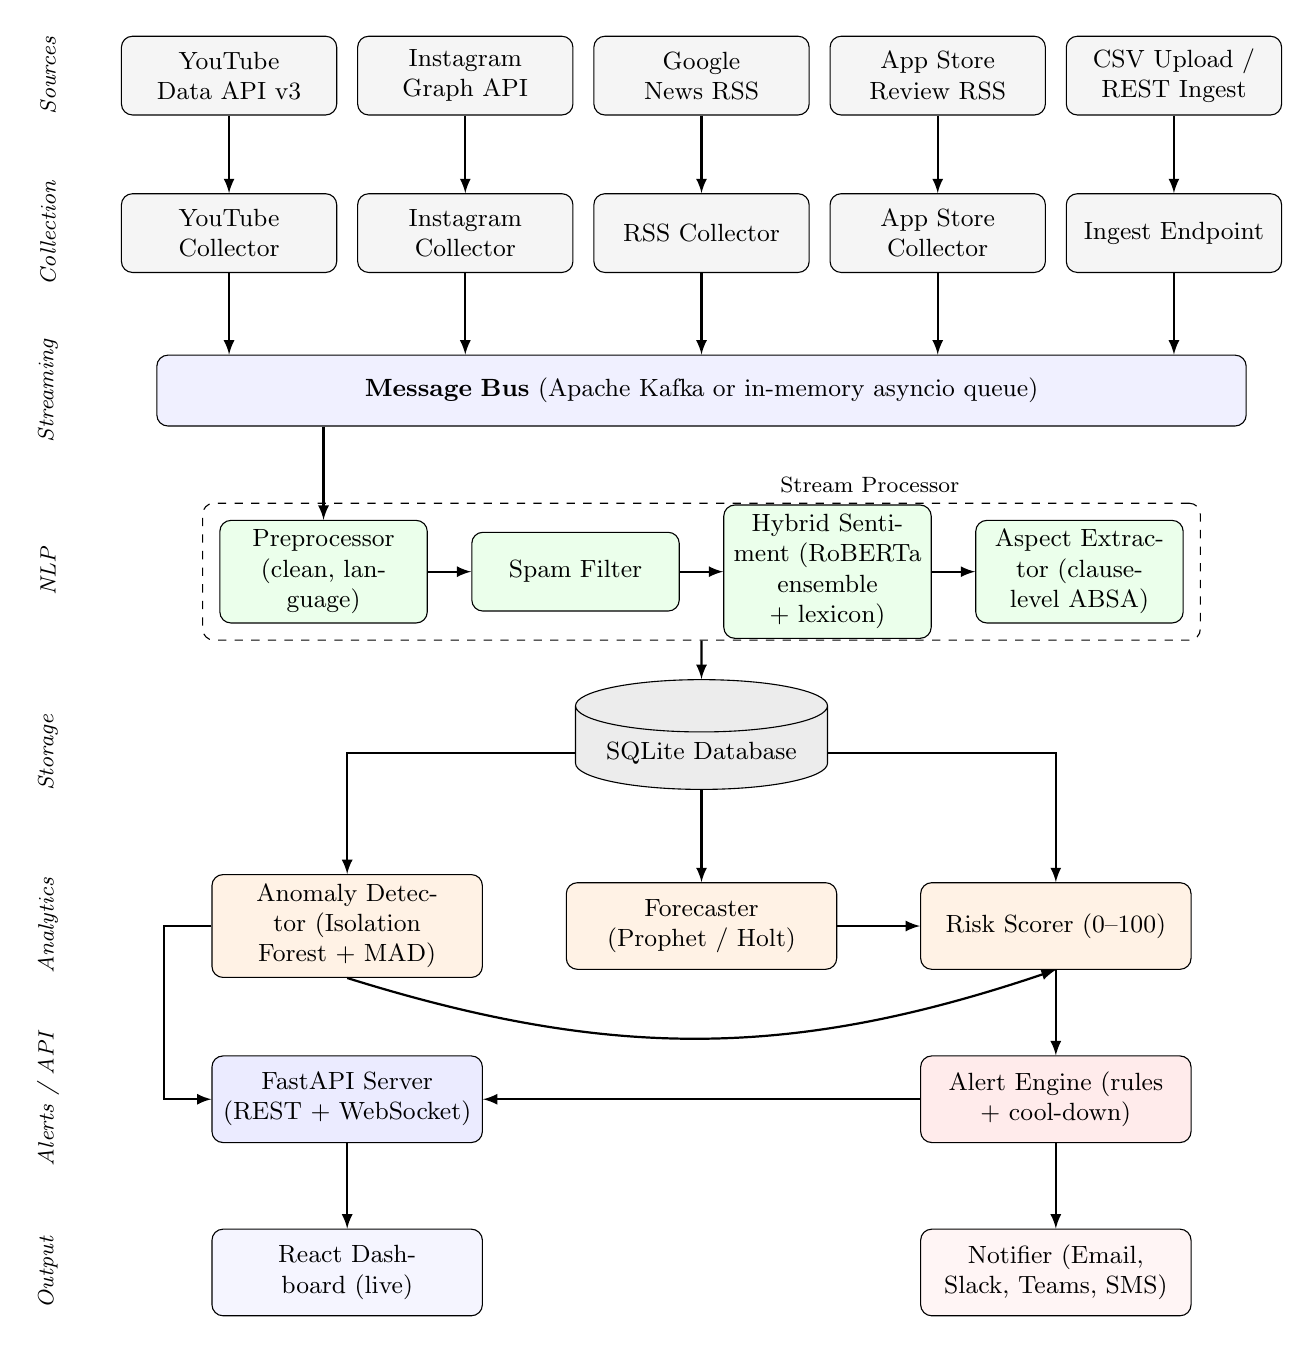
\begin{tikzpicture}[
    box/.style={draw, rounded corners, minimum height=1cm, text width=2.5cm, align=center, font=\small, fill=gray!8},
    wide/.style={draw, rounded corners, minimum height=0.9cm, text width=13.6cm, align=center, font=\small, fill=blue!6},
    proc/.style={draw, rounded corners, minimum height=1cm, text width=2.4cm, align=center, font=\small, fill=green!8},
    ana/.style={draw, rounded corners, minimum height=1.1cm, text width=3.2cm, align=center, font=\small, fill=orange!10},
    lbl/.style={font=\footnotesize\itshape, rotate=90, anchor=center},
    arr/.style={->, >=latex, thick}]

  % Row labels
  \node[lbl] at (-2.3,0) {Sources};
  \node[lbl] at (-2.3,-2) {Collection};
  \node[lbl] at (-2.3,-4) {Streaming};
  \node[lbl] at (-2.3,-6.3) {NLP};
  \node[lbl] at (-2.3,-8.6) {Storage};
  \node[lbl] at (-2.3,-10.8) {Analytics};
  \node[lbl] at (-2.3,-13) {Alerts / API};
  \node[lbl] at (-2.3,-15.2) {Output};

  % Sources
  \node[box] (s1) at (0,0) {YouTube Data API v3};
  \node[box] (s2) at (3,0) {Instagram Graph API};
  \node[box] (s3) at (6,0) {Google News RSS};
  \node[box] (s4) at (9,0) {App Store Review RSS};
  \node[box] (s5) at (12,0) {CSV Upload / REST Ingest};

  % Collectors
  \node[box] (c1) at (0,-2) {YouTube Collector};
  \node[box] (c2) at (3,-2) {Instagram Collector};
  \node[box] (c3) at (6,-2) {RSS Collector};
  \node[box] (c4) at (9,-2) {App Store Collector};
  \node[box] (c5) at (12,-2) {Ingest Endpoint};
  \foreach \i in {1,...,5} { \draw[arr] (s\i) -- (c\i); }

  % Bus
  \node[wide] (bus) at (6,-4) {\textbf{Message Bus} (Apache Kafka or in-memory asyncio queue)};
  \foreach \i in {1,...,5} { \draw[arr] (c\i) -- (c\i |- bus.north); }

  % NLP
  \node[proc] (p1) at (1.2,-6.3) {Preprocessor (clean, language)};
  \node[proc] (p2) at (4.4,-6.3) {Spam Filter};
  \node[proc] (p3) at (7.6,-6.3) {Hybrid Sentiment (RoBERTa ensemble + lexicon)};
  \node[proc] (p4) at (10.8,-6.3) {Aspect Extractor (clause-level ABSA)};
  \draw[arr] (p1) -- (p2); \draw[arr] (p2) -- (p3); \draw[arr] (p3) -- (p4);
  \node[draw, dashed, rounded corners, fit=(p1)(p4), inner sep=6pt, label={[font=\footnotesize]above right:Stream Processor}] (procbox) {};
  \draw[arr] (bus.south -| p1) -- (p1.north);

  % Storage
  \node[draw, cylinder, shape border rotate=90, aspect=0.25, minimum height=1.3cm, minimum width=3.2cm, fill=gray!15, align=center, font=\small] (db) at (6,-8.6) {SQLite Database};
  \draw[arr] (procbox.south -| db) -- (db.north);

  % Analytics
  \node[ana] (a1) at (1.5,-10.8) {Anomaly Detector (Isolation Forest + MAD)};
  \node[ana] (a2) at (6,-10.8) {Forecaster (Prophet / Holt)};
  \node[ana] (a3) at (10.5,-10.8) {Risk Scorer (0--100)};
  \draw[arr] (db.south) -- (a2.north);
  \draw[arr] (db.west) -| (a1.north);
  \draw[arr] (db.east) -| (a3.north);
  \draw[arr] (a2) -- (a3);
  \draw[arr] (a1.south) to[bend right=18] (a3.south);

  % Alerts and API
  \node[ana, fill=red!8] (al) at (10.5,-13) {Alert Engine (rules + cool-down)};
  \node[ana, fill=blue!8] (api) at (1.5,-13) {FastAPI Server (REST + WebSocket)};
  \draw[arr] (a3.south) -- (al.north);
  \draw[arr] (al.west) -- (api.east);
  \draw[arr] (a1.west) -- ++(-0.6,0) |- (api.west);

  % Output
  \node[ana, fill=red!4] (nt) at (10.5,-15.2) {Notifier (Email, Slack, Teams, SMS)};
  \node[ana, fill=blue!4] (ui) at (1.5,-15.2) {React Dashboard (live)};
  \draw[arr] (al) -- (nt);
  \draw[arr] (api) -- (ui);
\end{tikzpicture}}
\caption{BrandShield AI - Layered System Architecture}
\label{fig:architecture}
\end{figure}

The component diagram in Figure~\ref{fig:component} shows the same architecture from the point of view of the deployed software components and their dependencies.

\begin{figure}[!htbp]
\centering
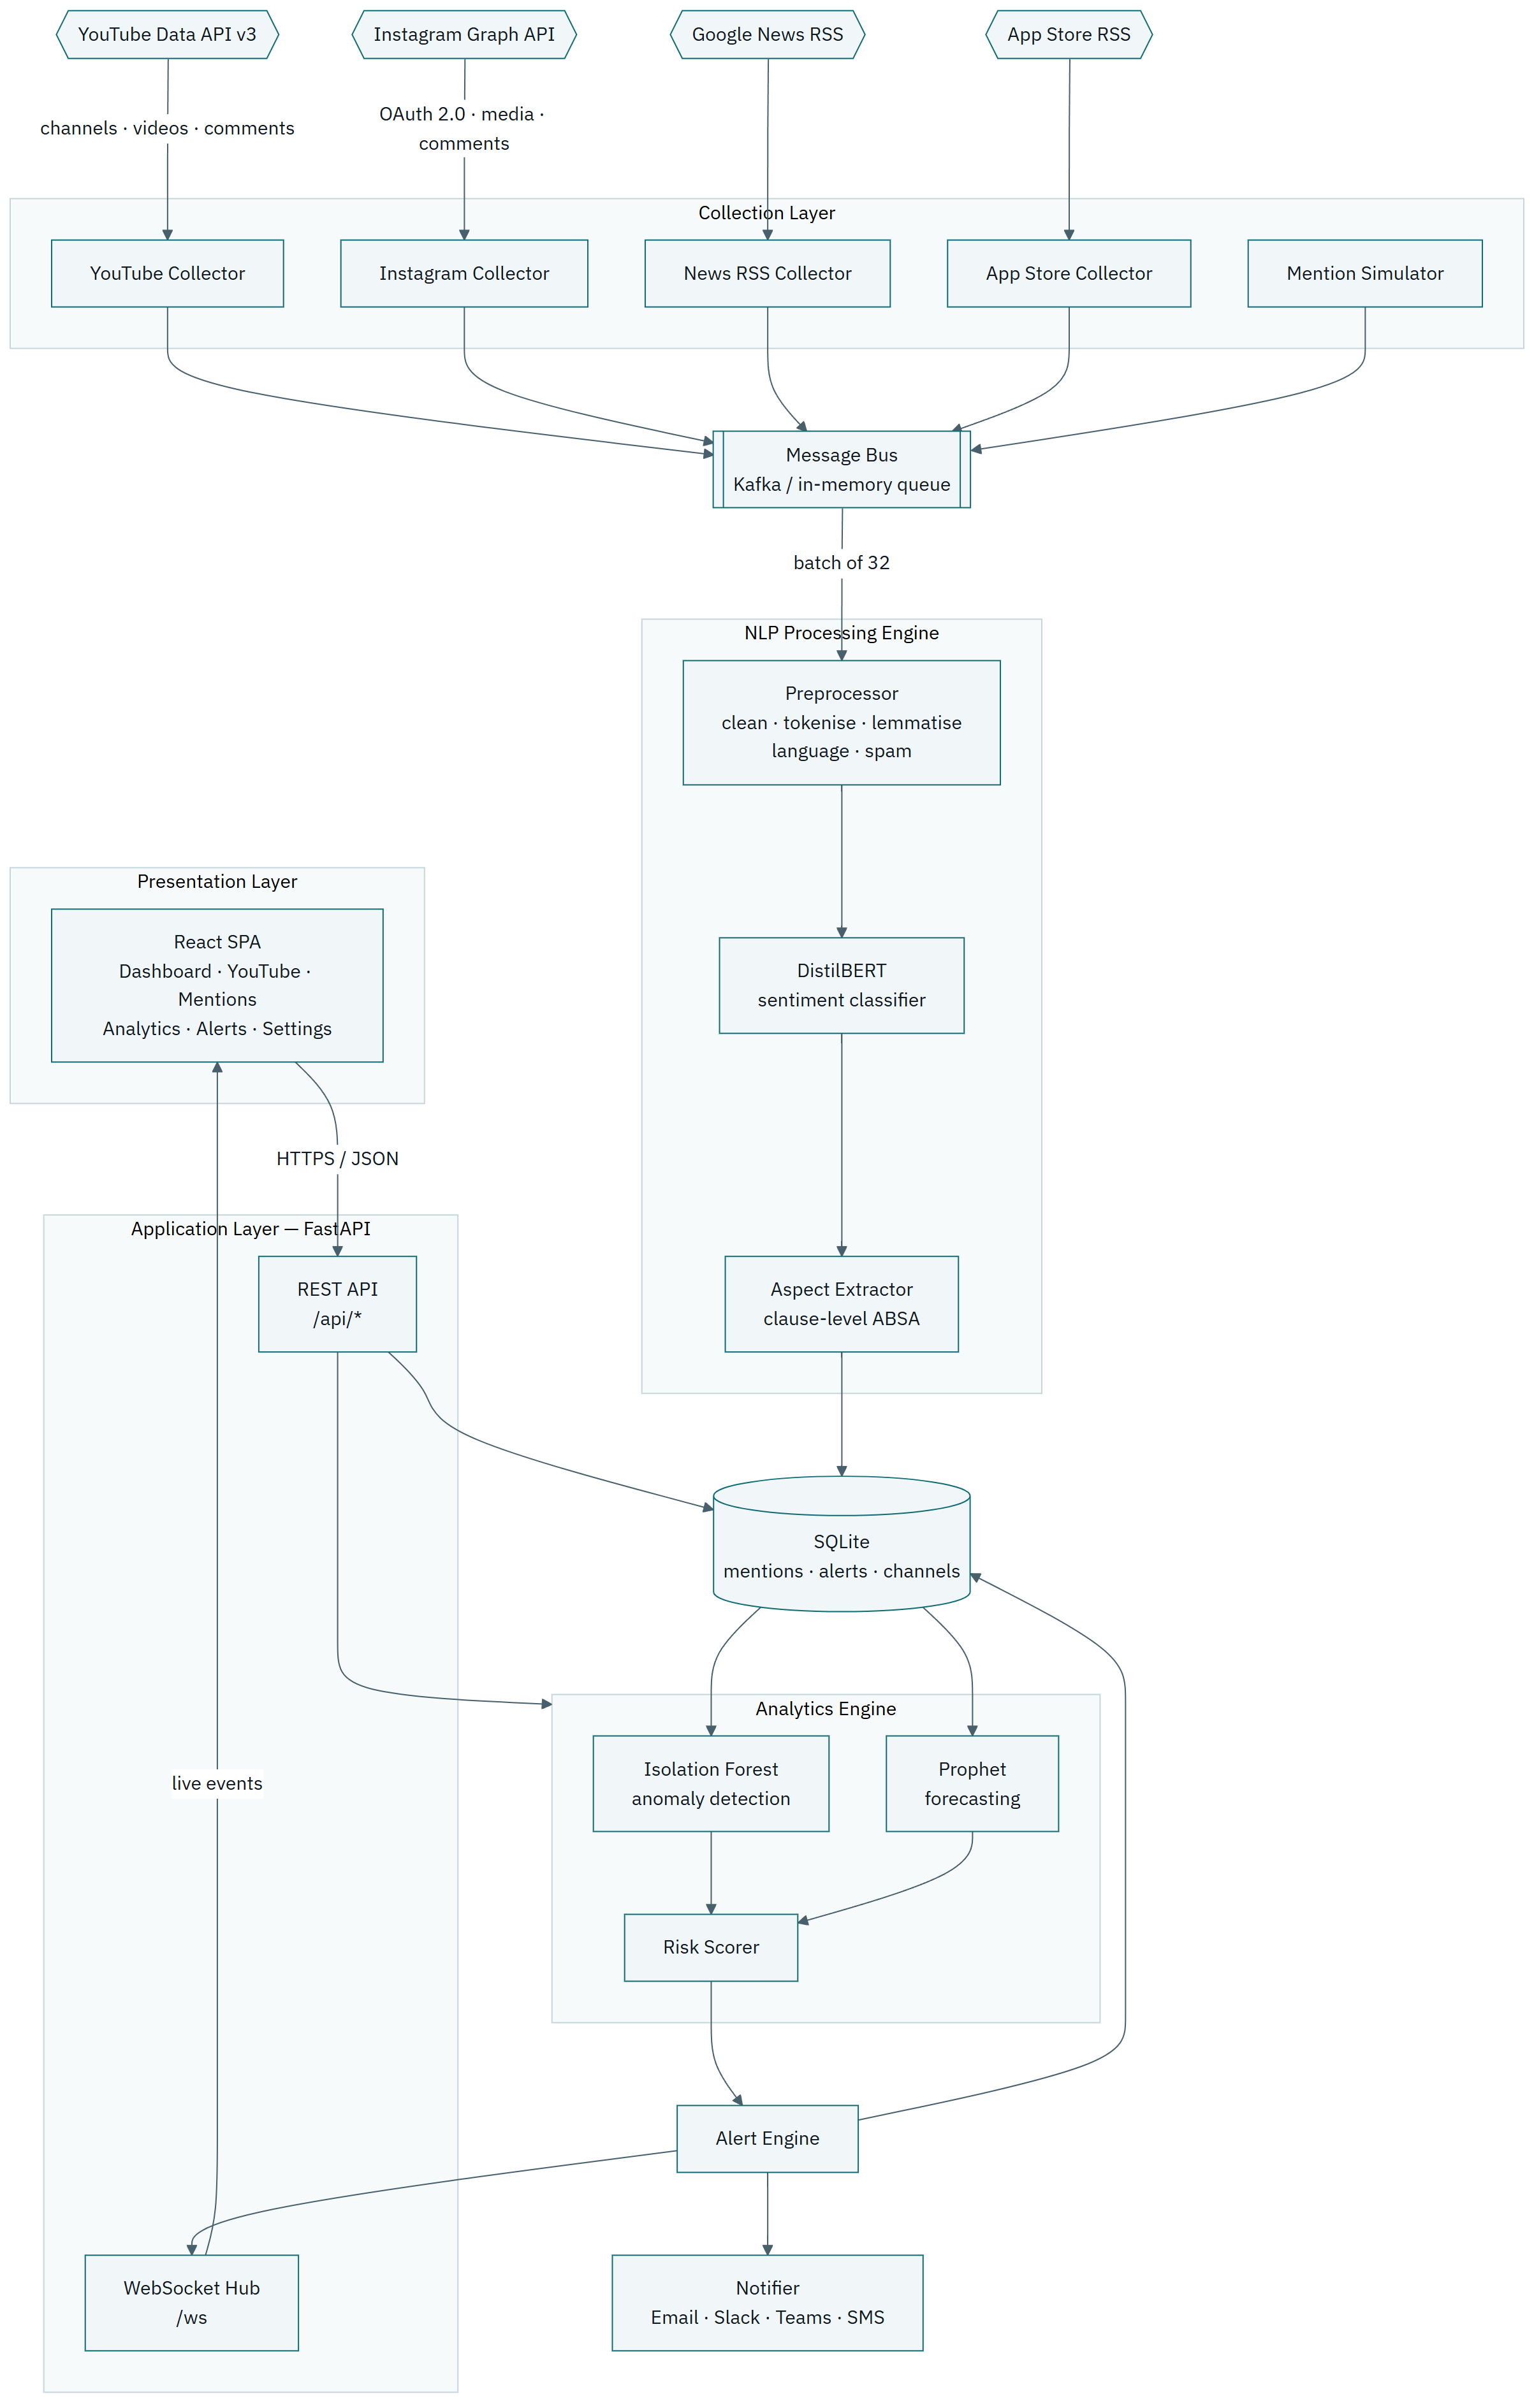
\includegraphics[width=\linewidth, height=17cm, keepaspectratio]{figures/03-component-diagram.png}
\caption{Component Diagram of BrandShield AI}
\label{fig:component}
\end{figure}

\subsection{Data Flow Diagrams}

Figure~\ref{fig:dfd0} is the context-level (Level 0) data flow diagram. It treats BrandShield AI as a single process and shows only the external entities it exchanges data with. Figure~\ref{fig:dfd1} breaks the system down into its five main processes and three data stores.

\lofsection{Data Flow Diagrams}
\begin{figure}[!htbp]
\centering
\resizebox{0.9\linewidth}{!}{%
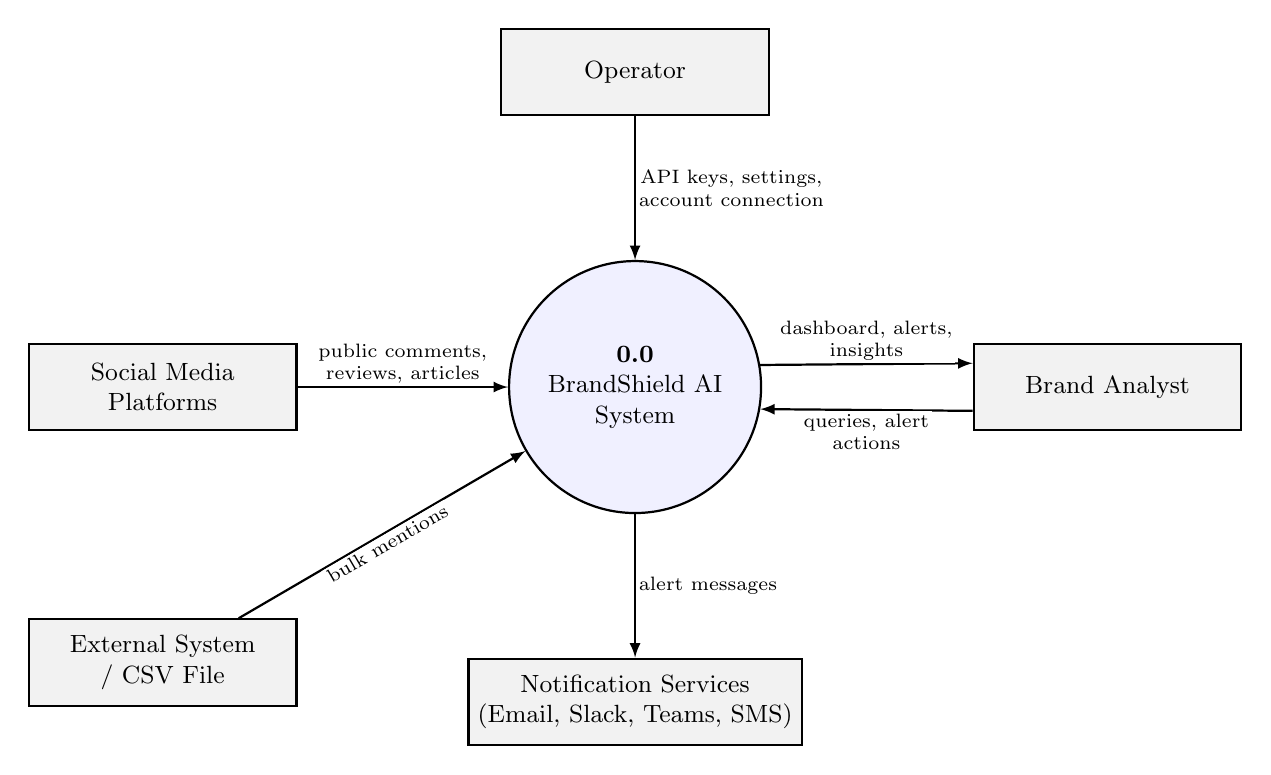
\begin{tikzpicture}[
    ent/.style={draw, thick, minimum width=3.4cm, minimum height=1.1cm, align=center, font=\small, fill=gray!10},
    pr/.style={draw, thick, circle, minimum size=3.2cm, align=center, font=\small, fill=blue!6},
    arr/.style={->, >=latex, thick},
    lab/.style={font=\scriptsize, align=center, fill=white, inner sep=1pt}]
  \node[pr] (sys) at (0,0) {\textbf{0.0}\\BrandShield AI\\System};
  \node[ent] (plat) at (-6,0) {Social Media\\Platforms};
  \node[ent] (an) at (6,0) {Brand Analyst};
  \node[ent] (op) at (0,4) {Operator};
  \node[ent] (ns) at (0,-4) {Notification Services\\(Email, Slack, Teams, SMS)};
  \node[ent] (ext) at (-6,-3.5) {External System\\/ CSV File};

  \draw[arr] (plat) -- node[lab, above]{public comments,\\reviews, articles} (sys);
  \draw[arr] (ext) -- node[lab, sloped, below]{bulk mentions} (sys);
  \draw[arr] (op) -- node[lab, right]{API keys, settings,\\account connection} (sys);
  \draw[arr] (sys) -- node[lab, right]{alert messages} (ns);
  \draw[arr] (sys.10) -- node[lab, above]{dashboard, alerts,\\insights} (an.170);
  \draw[arr] (an.190) -- node[lab, below]{queries, alert\\actions} (sys.350);
\end{tikzpicture}}
\caption{DFD Level 0 (Context Diagram)}
\label{fig:dfd0}
\end{figure}

\begin{figure}[!htbp]
\centering
\resizebox{\linewidth}{!}{%
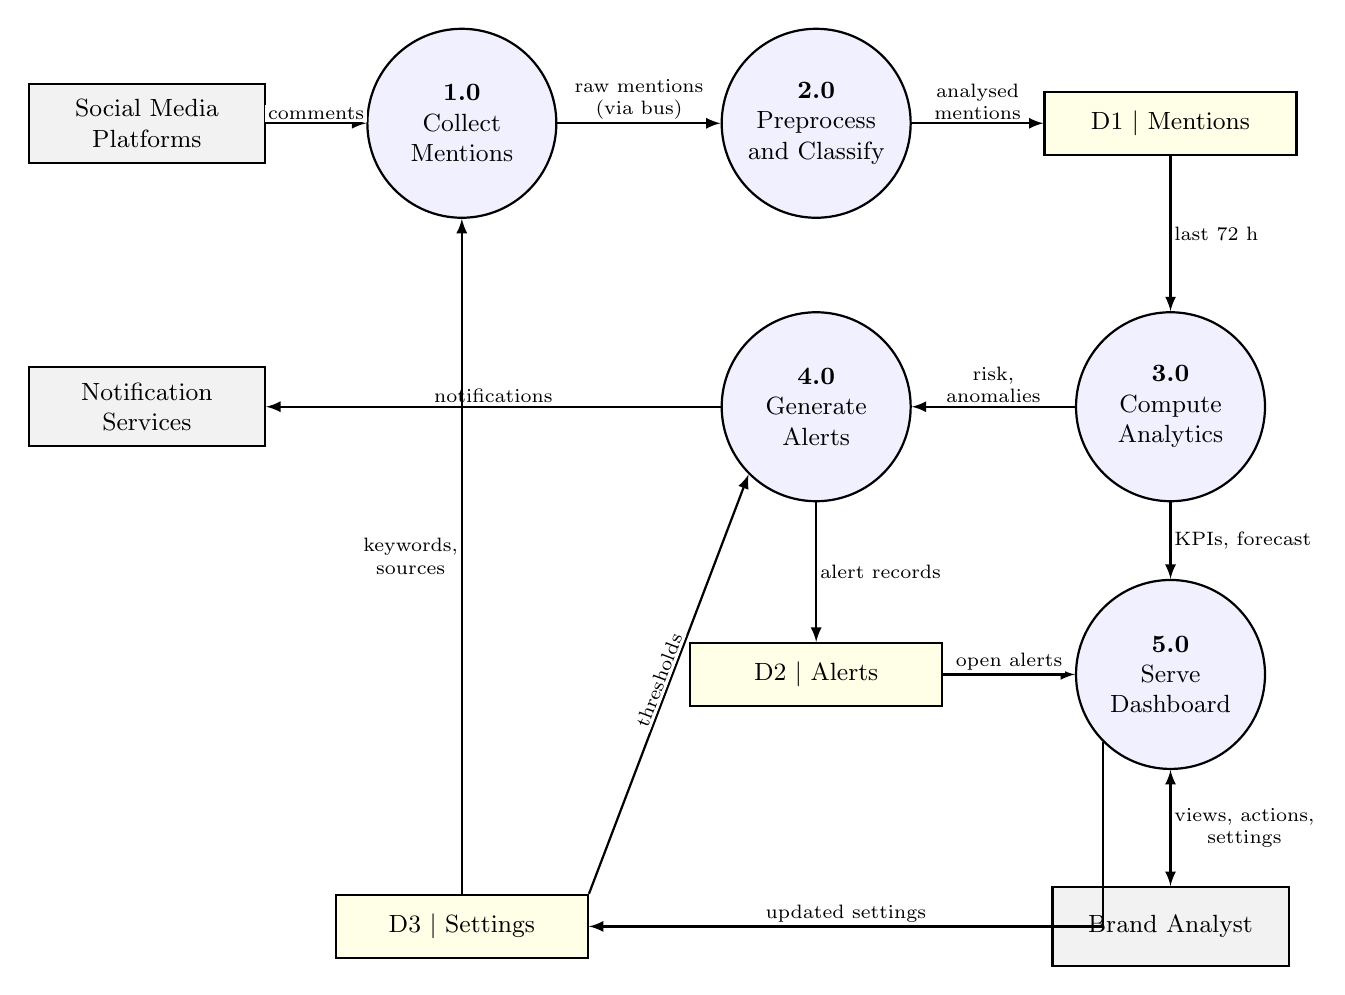
\begin{tikzpicture}[
    ent/.style={draw, thick, minimum width=3cm, minimum height=1cm, align=center, font=\small, fill=gray!10},
    pr/.style={draw, thick, circle, minimum size=2.4cm, align=center, font=\small, fill=blue!6},
    st/.style={draw, thick, minimum width=3.2cm, minimum height=0.8cm, align=center, font=\small, fill=yellow!10},
    arr/.style={->, >=latex, thick},
    lab/.style={font=\scriptsize, align=center, fill=white, inner sep=1pt}]
  \node[ent] (e1) at (0,0) {Social Media\\Platforms};
  \node[pr] (p1) at (4,0) {\textbf{1.0}\\Collect\\Mentions};
  \node[pr] (p2) at (8.5,0) {\textbf{2.0}\\Preprocess\\and Classify};
  \node[st] (d1) at (13,0) {D1 \textbar{} Mentions};
  \node[pr] (p3) at (13,-3.6) {\textbf{3.0}\\Compute\\Analytics};
  \node[pr] (p4) at (8.5,-3.6) {\textbf{4.0}\\Generate\\Alerts};
  \node[ent] (e2) at (0,-3.6) {Notification\\Services};
  \node[st] (d2) at (8.5,-7) {D2 \textbar{} Alerts};
  \node[pr] (p5) at (13,-7) {\textbf{5.0}\\Serve\\Dashboard};
  \node[ent] (e3) at (13,-10.2) {Brand Analyst};
  \node[st] (d3) at (4,-10.2) {D3 \textbar{} Settings};

  \draw[arr] (e1) -- node[lab, above]{comments} (p1);
  \draw[arr] (p1) -- node[lab, above]{raw mentions\\(via bus)} (p2);
  \draw[arr] (p2) -- node[lab, above]{analysed\\mentions} (d1);
  \draw[arr] (d1) -- node[lab, right]{last 72 h} (p3);
  \draw[arr] (p3) -- node[lab, above]{risk,\\anomalies} (p4);
  \draw[arr] (p4) -- node[lab, above]{notifications} (e2);
  \draw[arr] (p4) -- node[lab, right]{alert records} (d2);
  \draw[arr] (d2) -- node[lab, above]{open alerts} (p5);
  \draw[arr] (p3) -- node[lab, right]{KPIs, forecast} (p5);
  \draw[<->, >=latex, thick] (p5) -- node[lab, right]{views, actions,\\settings} (e3);
  \draw[arr] (p5.south west) |- node[lab, pos=0.75, above]{updated settings} (d3.east);
  \draw[arr] (d3) -- node[lab, left]{keywords,\\sources} (p1);
  \draw[arr] (d3.north east) -- node[lab, sloped, above]{thresholds} (p4.south west);
\end{tikzpicture}}
\caption{DFD Level 1}
\label{fig:dfd1}
\end{figure}

\section{Overview of Project Modules}

The source code is organised into the following modules.

\textbf{1. Application Core.} The \texttt{App} class wires every component together when the server starts. It creates the database, the message bus, the NLP models and the services, and it launches the background tasks: collector loops, the stream processor, the analytics loop (every 30 s), the forecast loop (every 5 min) and the metrics loop (every 5 s).

\textbf{2. Configuration.} Static settings such as API keys and file paths are read from environment variables. Runtime settings such as the brand name, keywords, thresholds and aspects are stored in the database and can be changed from the dashboard. Changes are validated and take effect immediately.

\textbf{3. Collectors.} Each data source has a collector that implements a common interface with three methods: \texttt{configured()}, \texttt{status()} and \texttt{poll()}. Adding a new platform only requires writing one new class. There is also a simulator that generates realistic brand comments and can inject a crisis on a chosen aspect for demonstrations.

\textbf{4. Social Integrations.} The YouTube service resolves a channel from its handle, keeps track of its videos, and only re-downloads comments for videos whose comment count has changed. This keeps the system within the free daily quota. The Instagram service handles the OAuth login, stores the access token in encrypted form, refreshes it before it expires, and syncs comments on the account's posts. A small tunnel manager starts a temporary HTTPS address, which Meta requires for the OAuth redirect during local development.

\textbf{5. Streaming Pipeline.} The message bus has two interchangeable implementations: Kafka for distributed use and an in-memory queue (capacity 50,000) for single-machine use. The processor reads batches of up to 32 mentions, waiting at most half a second to fill a batch. It normalises them, removes duplicates, runs the NLP steps and saves the results. A hub broadcasts new mentions, risk updates and alerts to every open dashboard over WebSocket.

\textbf{6. NLP Engine.} This module has three parts: the text preprocessor, the hybrid sentiment model and the aspect extractor. They are described in detail in Section~\ref{sec:algo}.

\textbf{7. Analytics Engine.} The analytics service loads the last 72 hours of mentions, groups them into 15-minute buckets, runs the anomaly detector, groups anomalous buckets into incidents, computes the risk score, and produces the KPIs, trends and aspect tables shown on the dashboard.

\textbf{8. Alert Engine.} Seven rules turn analytic results into alerts. Every alert has a de-duplication key and a cool-down period, so one incident produces one alert and not a stream of identical messages. The notifier sends alerts above a chosen severity to the configured channels.

\textbf{9. Storage.} A single module holds the database schema, migrations and data access functions. All queries are parameterised.

\textbf{10. Dashboard.} The React frontend with ten pages, a shared live-data context and an API client.

\section{User Interface}

The dashboard is the part of the system that brand managers actually see, so we spent considerable time making it clear rather than crowded. It uses a newspaper-style layout with a light paper theme and an optional dark theme, a headline that states the brand's situation in one sentence, large summary numbers, and colour coding that is consistent everywhere: green for positive, grey for neutral and red for negative. The screens are listed below.

\lofsection{User Interface Screens}

\begin{figure}[!htbp]
\centering
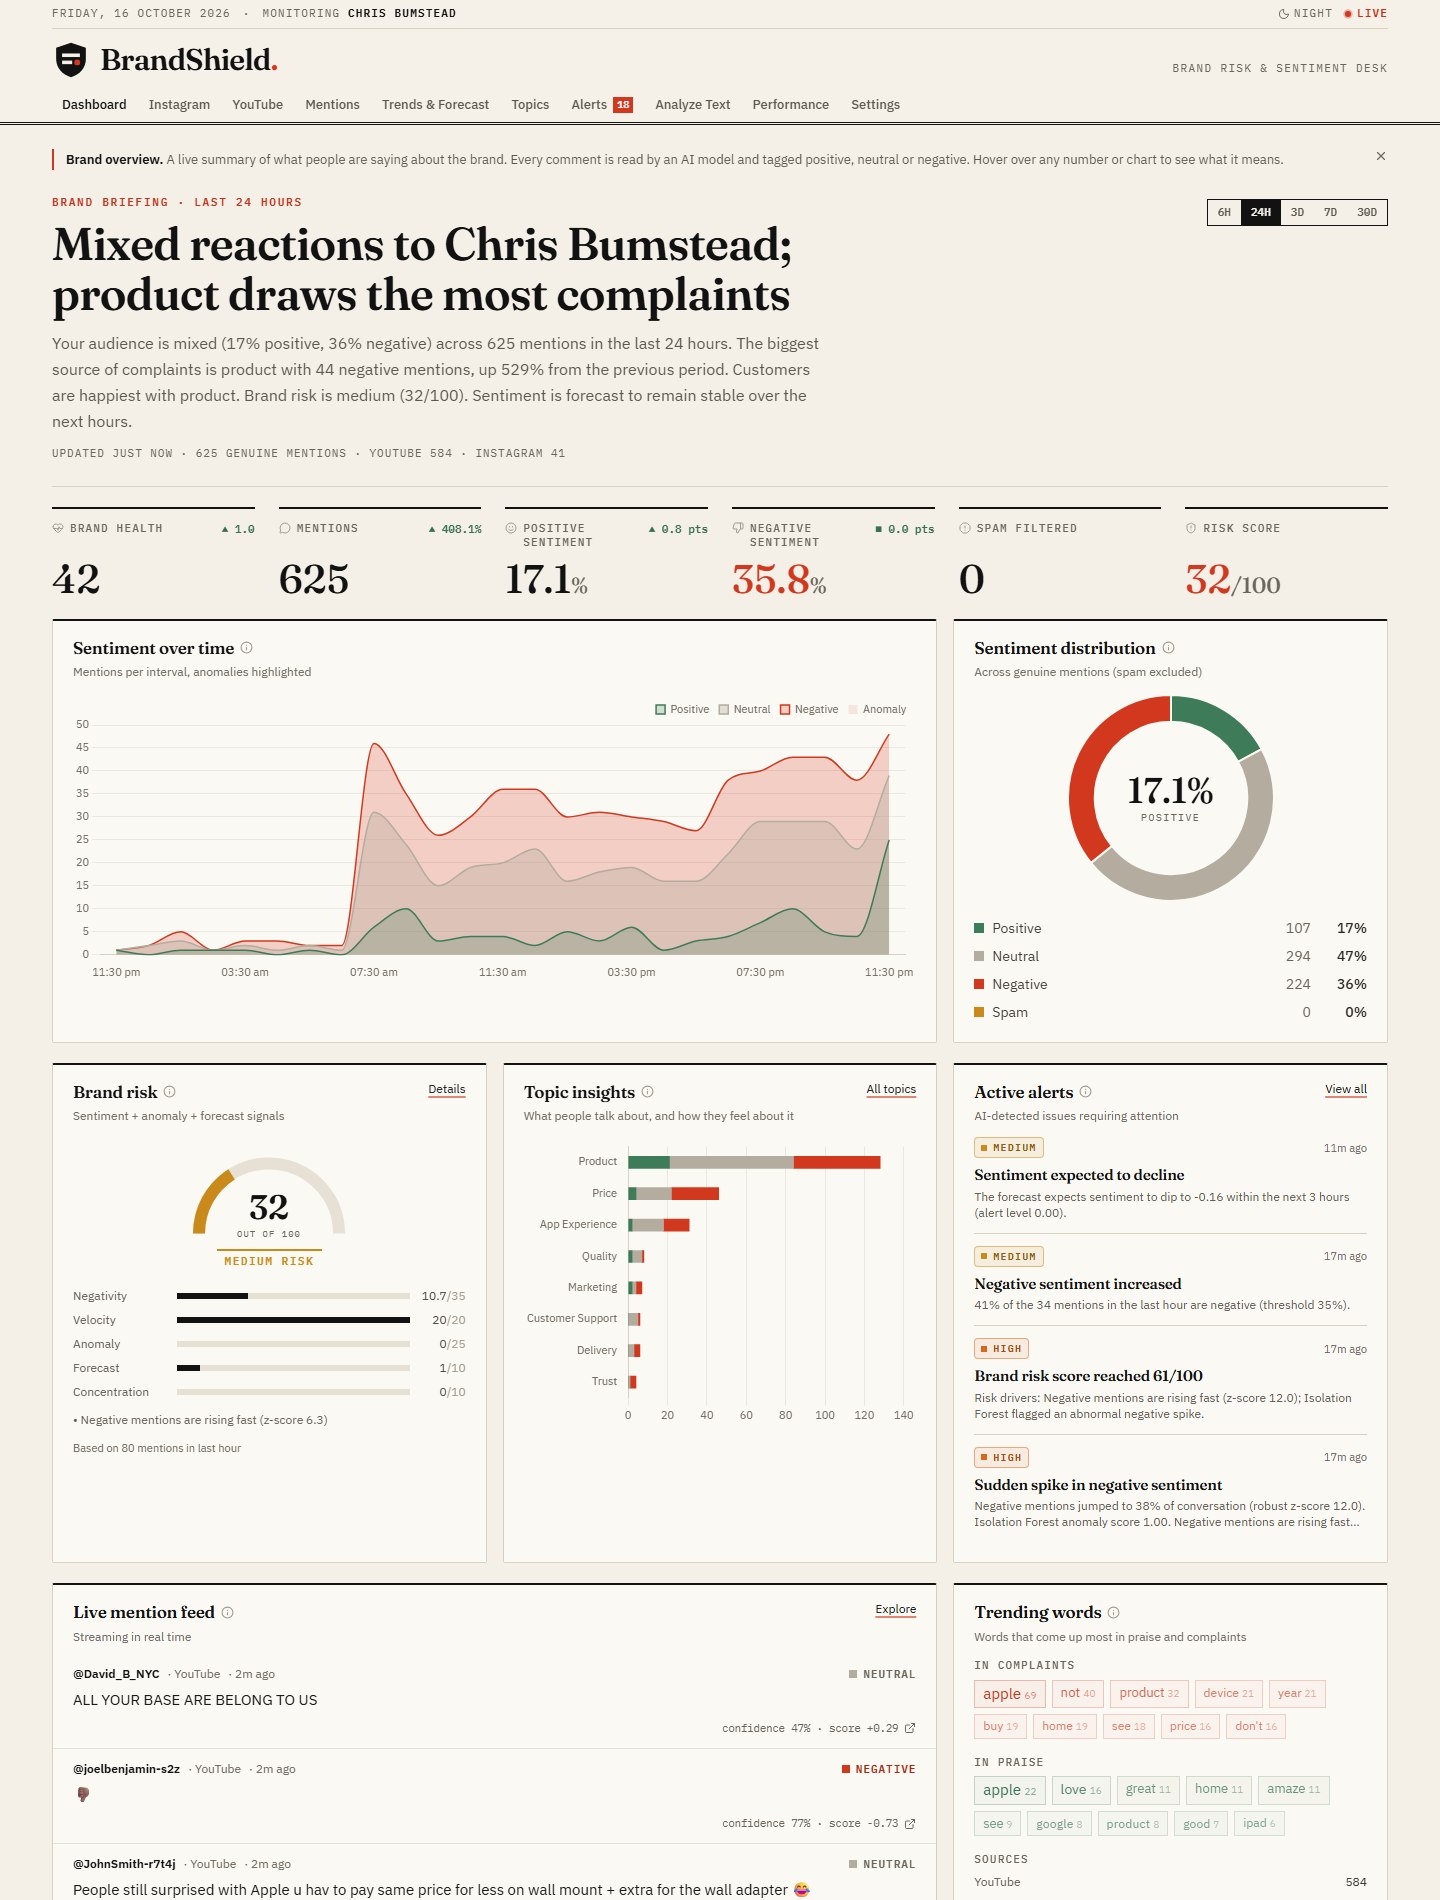
\includegraphics[width=\linewidth,height=0.45\textheight,keepaspectratio]{figures/ui-dashboard.png}
\caption{Main Dashboard}
\label{fig:ui-dashboard}
\end{figure}

\textbf{Dashboard.} The home page answers the question ``how are we doing right now?'' It opens with a headline generated from the numbers, for example ``Mixed reactions to Apple; product draws the most complaints'', followed by total mentions, the positive, neutral and negative split, brand health, and the risk score as a gauge, each compared with the previous period. An automatically generated text summary describes the main changes in plain English. A live feed at the bottom shows new comments as they are analysed.

\begin{figure}[!htbp]
\centering
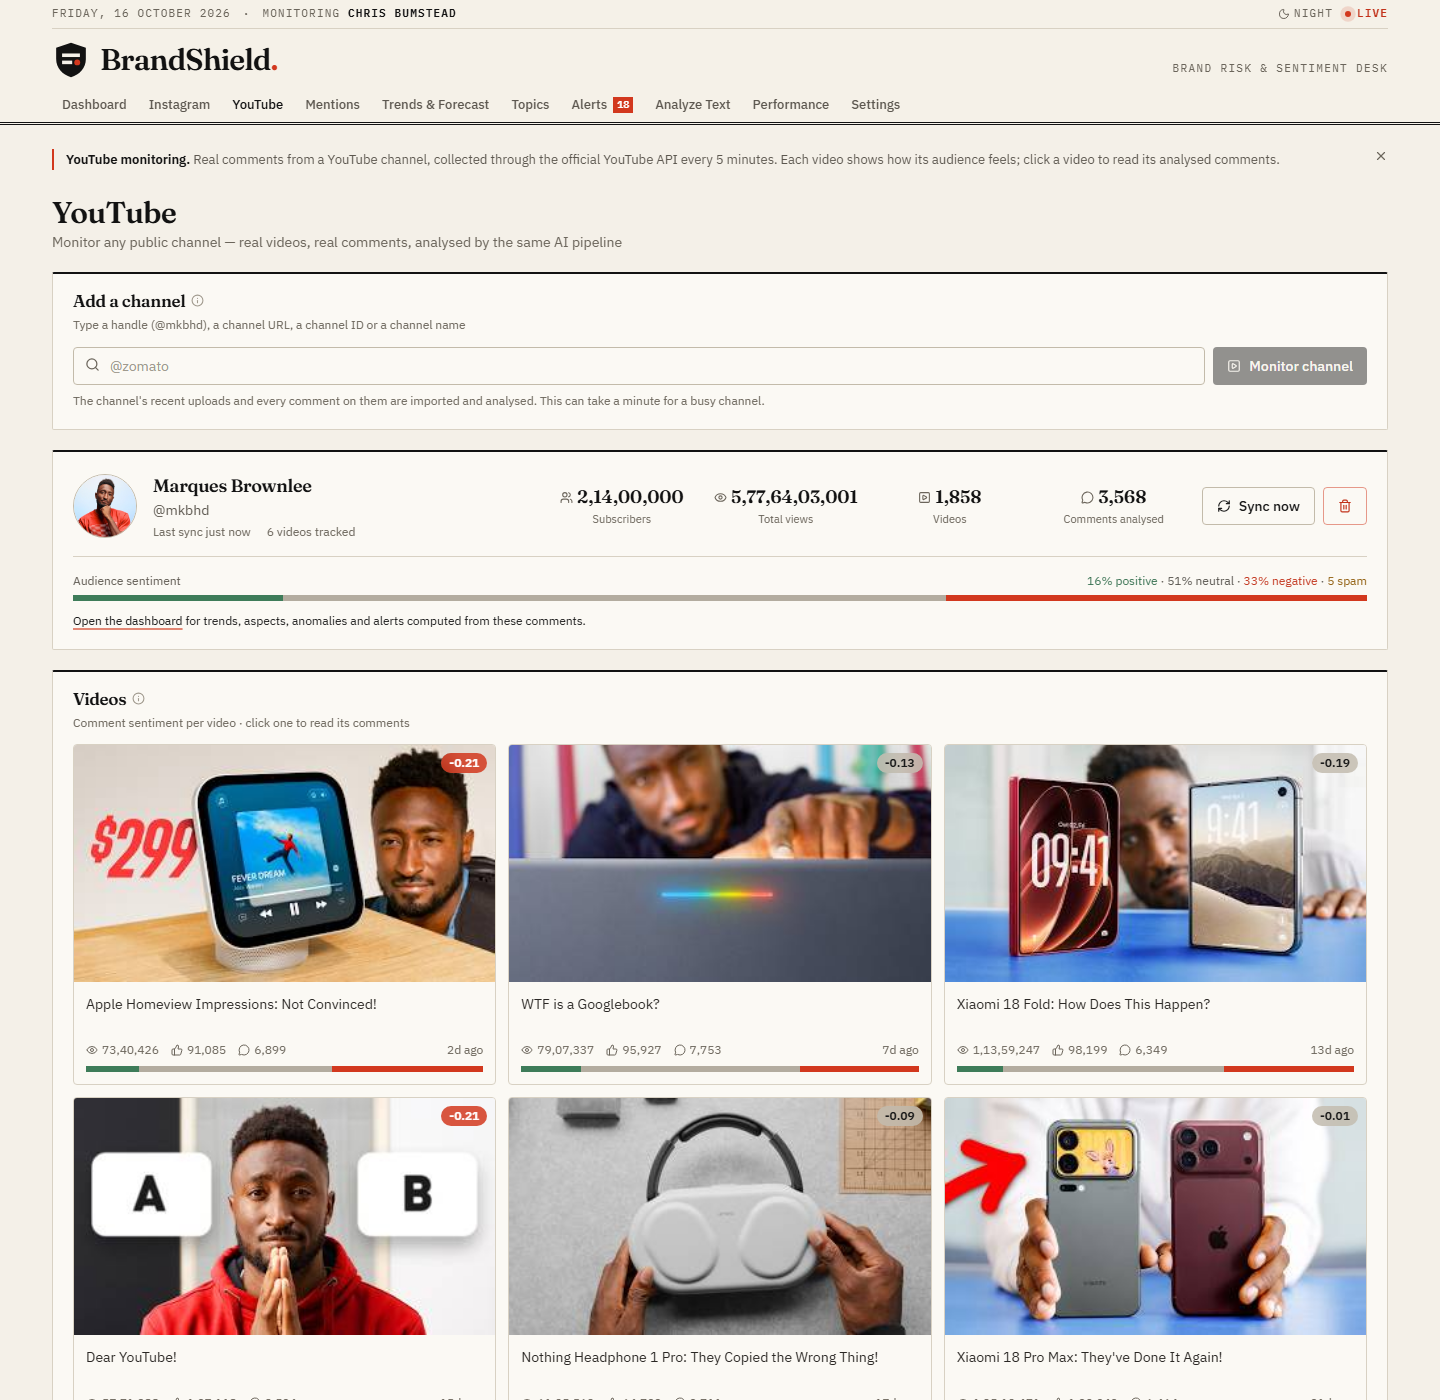
\includegraphics[width=\linewidth,height=0.45\textheight,keepaspectratio]{figures/ui-youtube.png}
\caption{YouTube Channel Monitoring}
\label{fig:ui-youtube}
\end{figure}

\begin{figure}[!htbp]
\centering
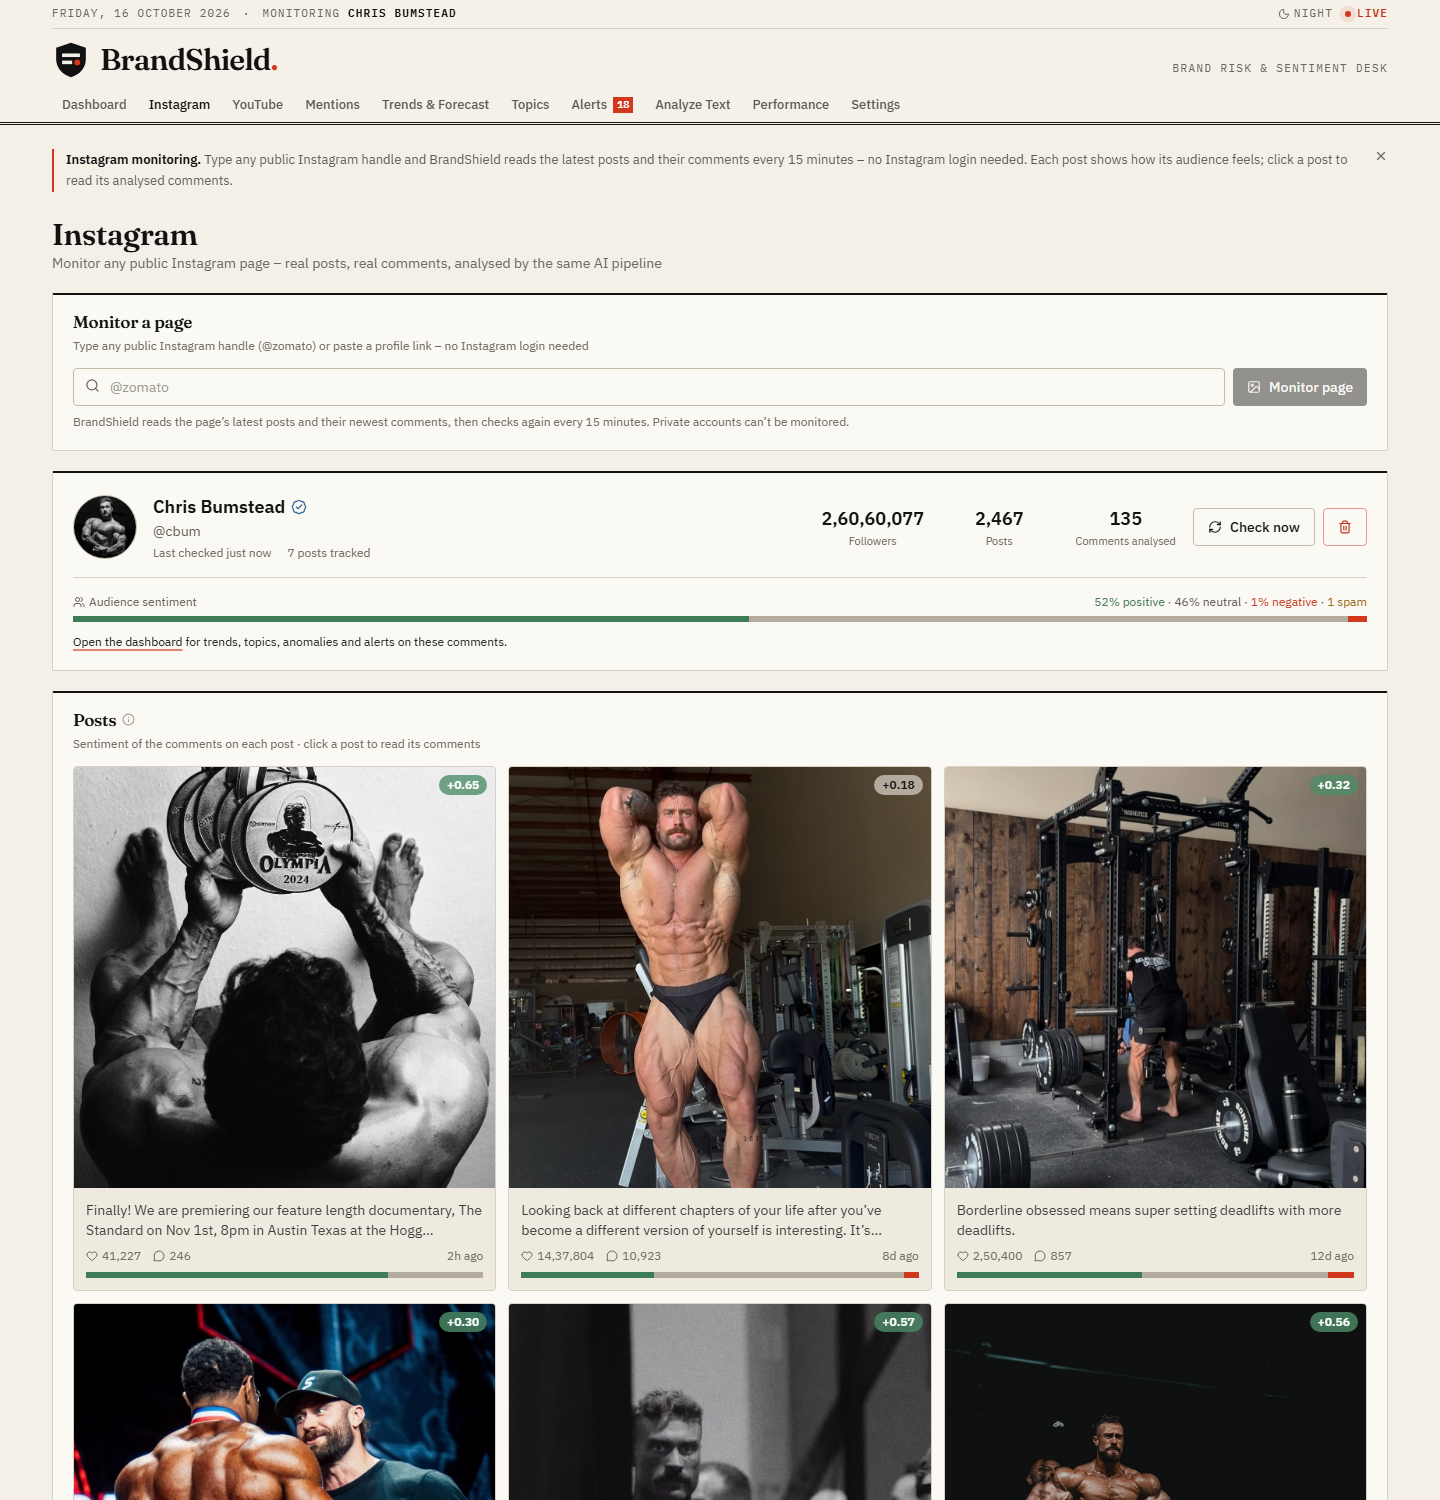
\includegraphics[width=\linewidth,height=0.45\textheight,keepaspectratio]{figures/ui-instagram.png}
\caption{Instagram Page Monitoring}
\label{fig:ui-instagram}
\end{figure}

\textbf{YouTube and Instagram.} These pages let the user add sources without touching any configuration file or API key; keys are set once by the operator on a separate Server setup page. On the YouTube page the user types a channel handle. On the Instagram page the user types any public page handle, and the page's latest posts and comments are read through a third-party data service (Apify), since the official API only covers the user's own account; a brand can still connect its own Business account through Instagram's official login. Both pages then show each video or post with its own sentiment breakdown.

\begin{figure}[!htbp]
\centering
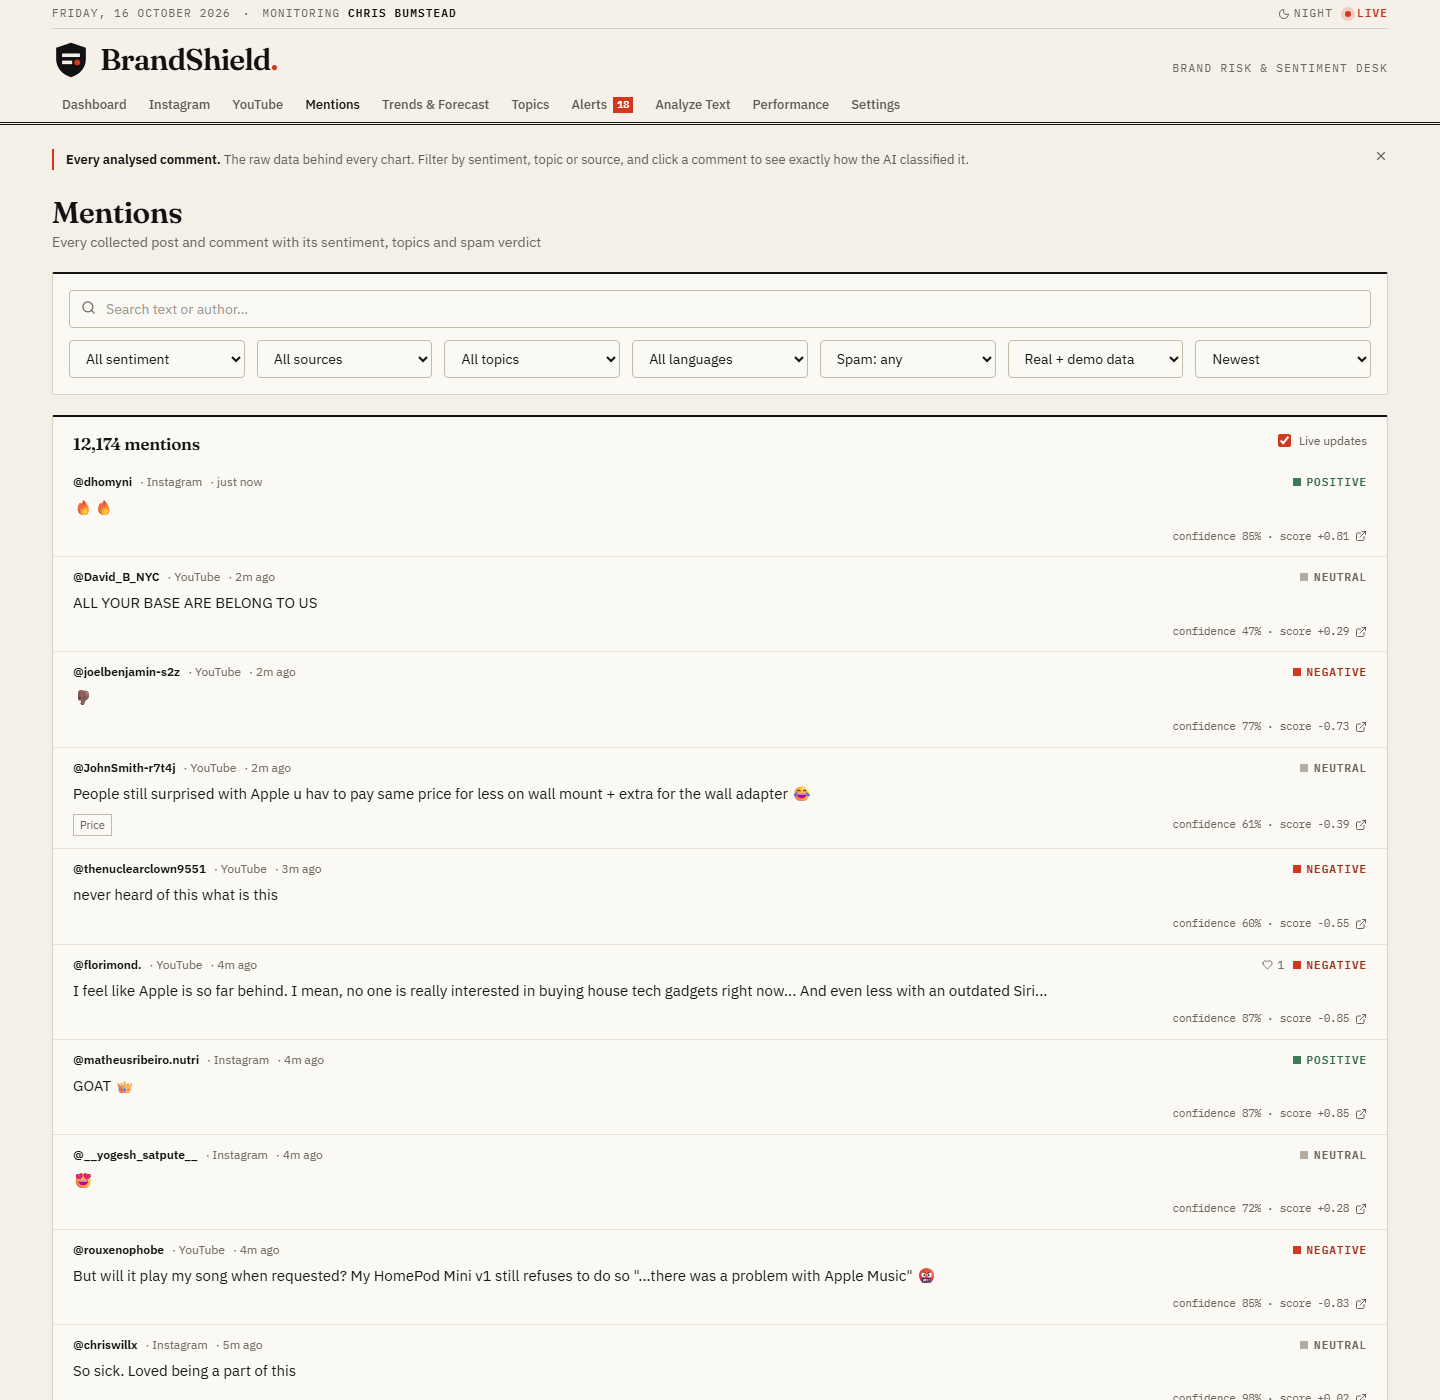
\includegraphics[width=\linewidth,height=0.45\textheight,keepaspectratio]{figures/ui-mentions.png}
\caption{Mentions Explorer}
\label{fig:ui-mentions}
\end{figure}

\textbf{Mentions.} A searchable, filterable list of every analysed comment. Expanding a mention shows its class probabilities, the aspects found and the exact clause each aspect came from.

\begin{figure}[!htbp]
\centering
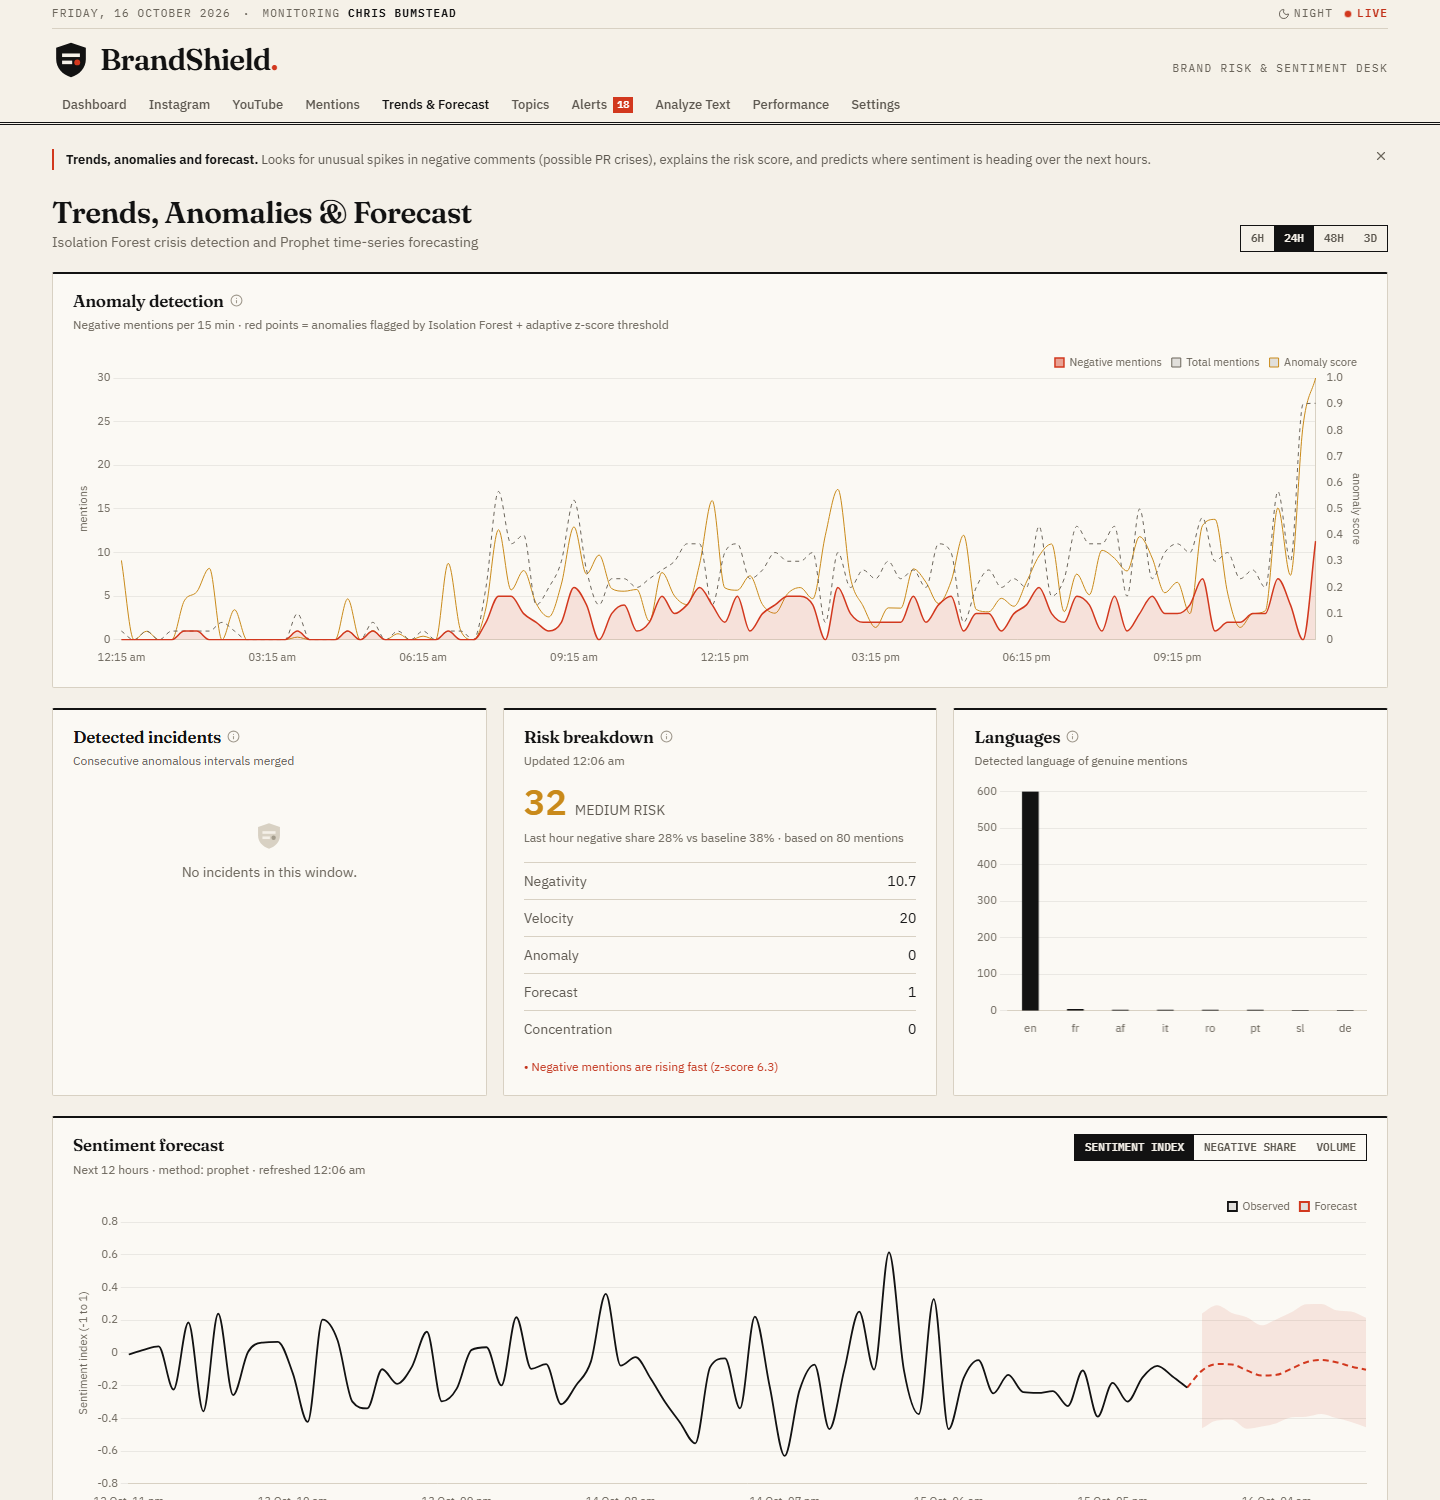
\includegraphics[width=\linewidth,height=0.45\textheight,keepaspectratio]{figures/ui-trends.png}
\caption{Trends and Forecast}
\label{fig:ui-trends}
\end{figure}

\begin{figure}[!htbp]
\centering
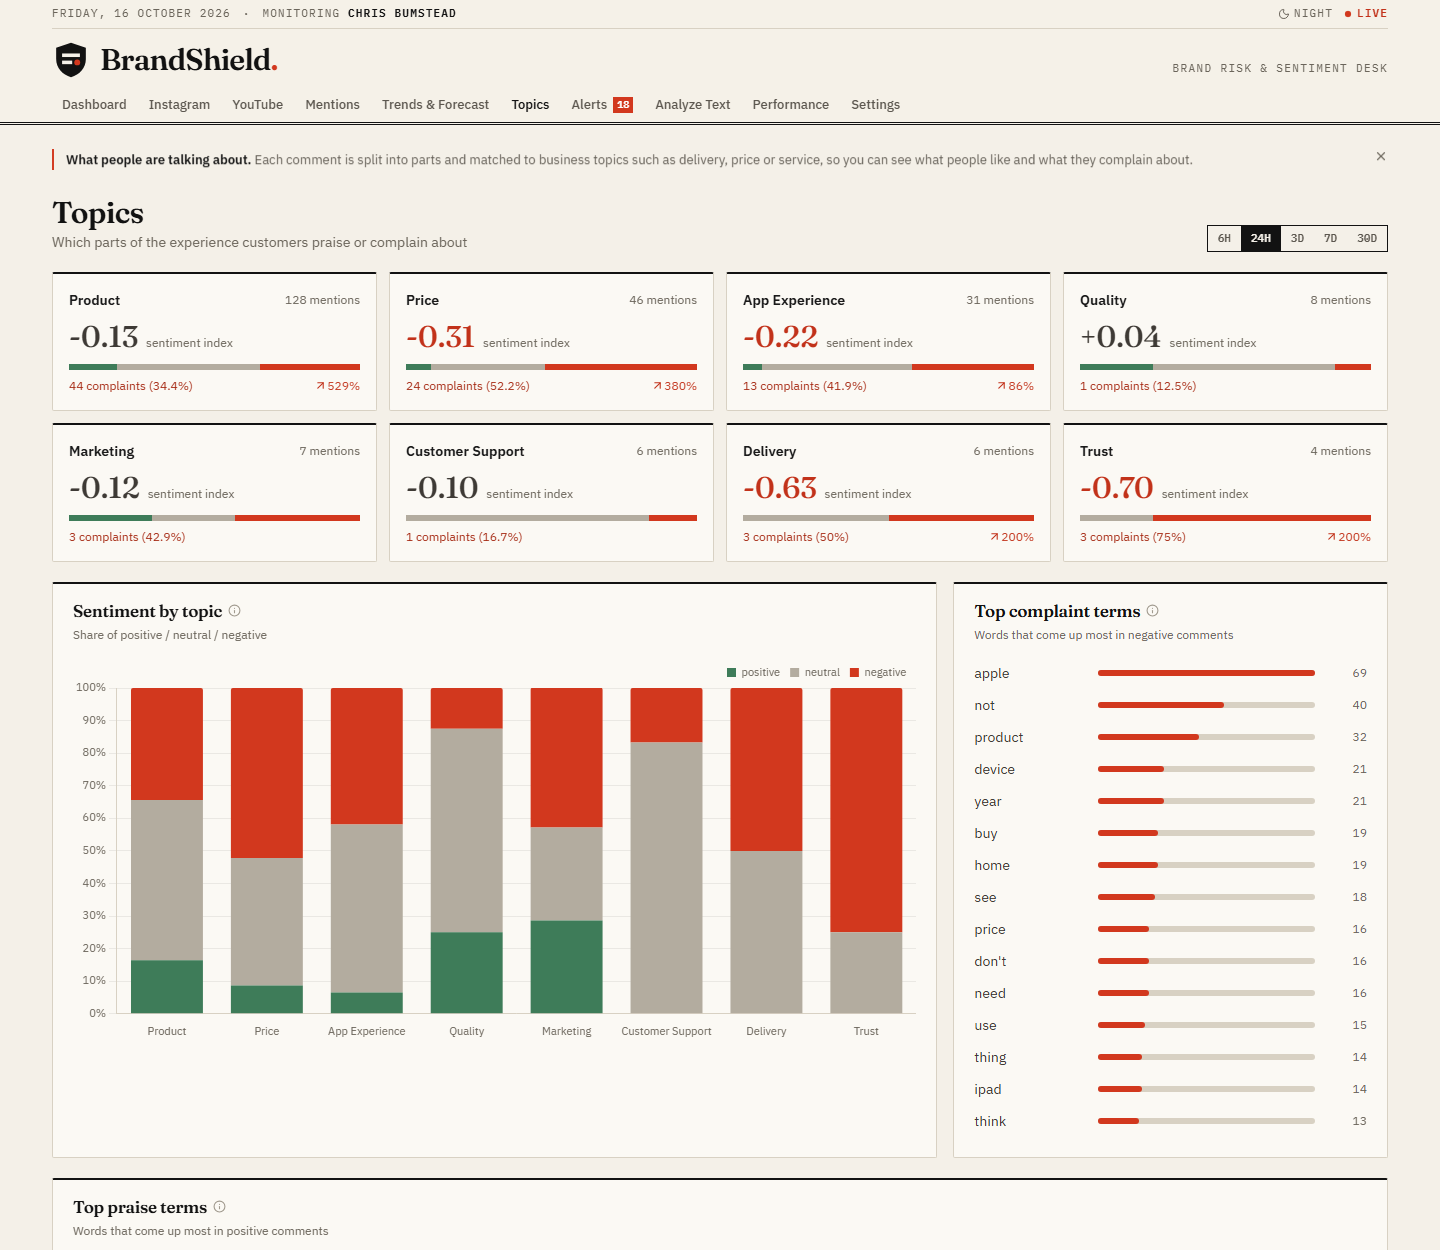
\includegraphics[width=\linewidth,height=0.45\textheight,keepaspectratio]{figures/ui-topics.png}
\caption{Topics}
\label{fig:ui-aspects}
\end{figure}

\textbf{Trends and Forecast, Topics.} These two pages explain \textit{why} the numbers on the dashboard look the way they do. The trends page marks anomalous windows on the chart and lists incidents; the Topics page (aspect-based sentiment) shows which aspects of the business are drawing the most complaints.

\begin{figure}[!htbp]
\centering
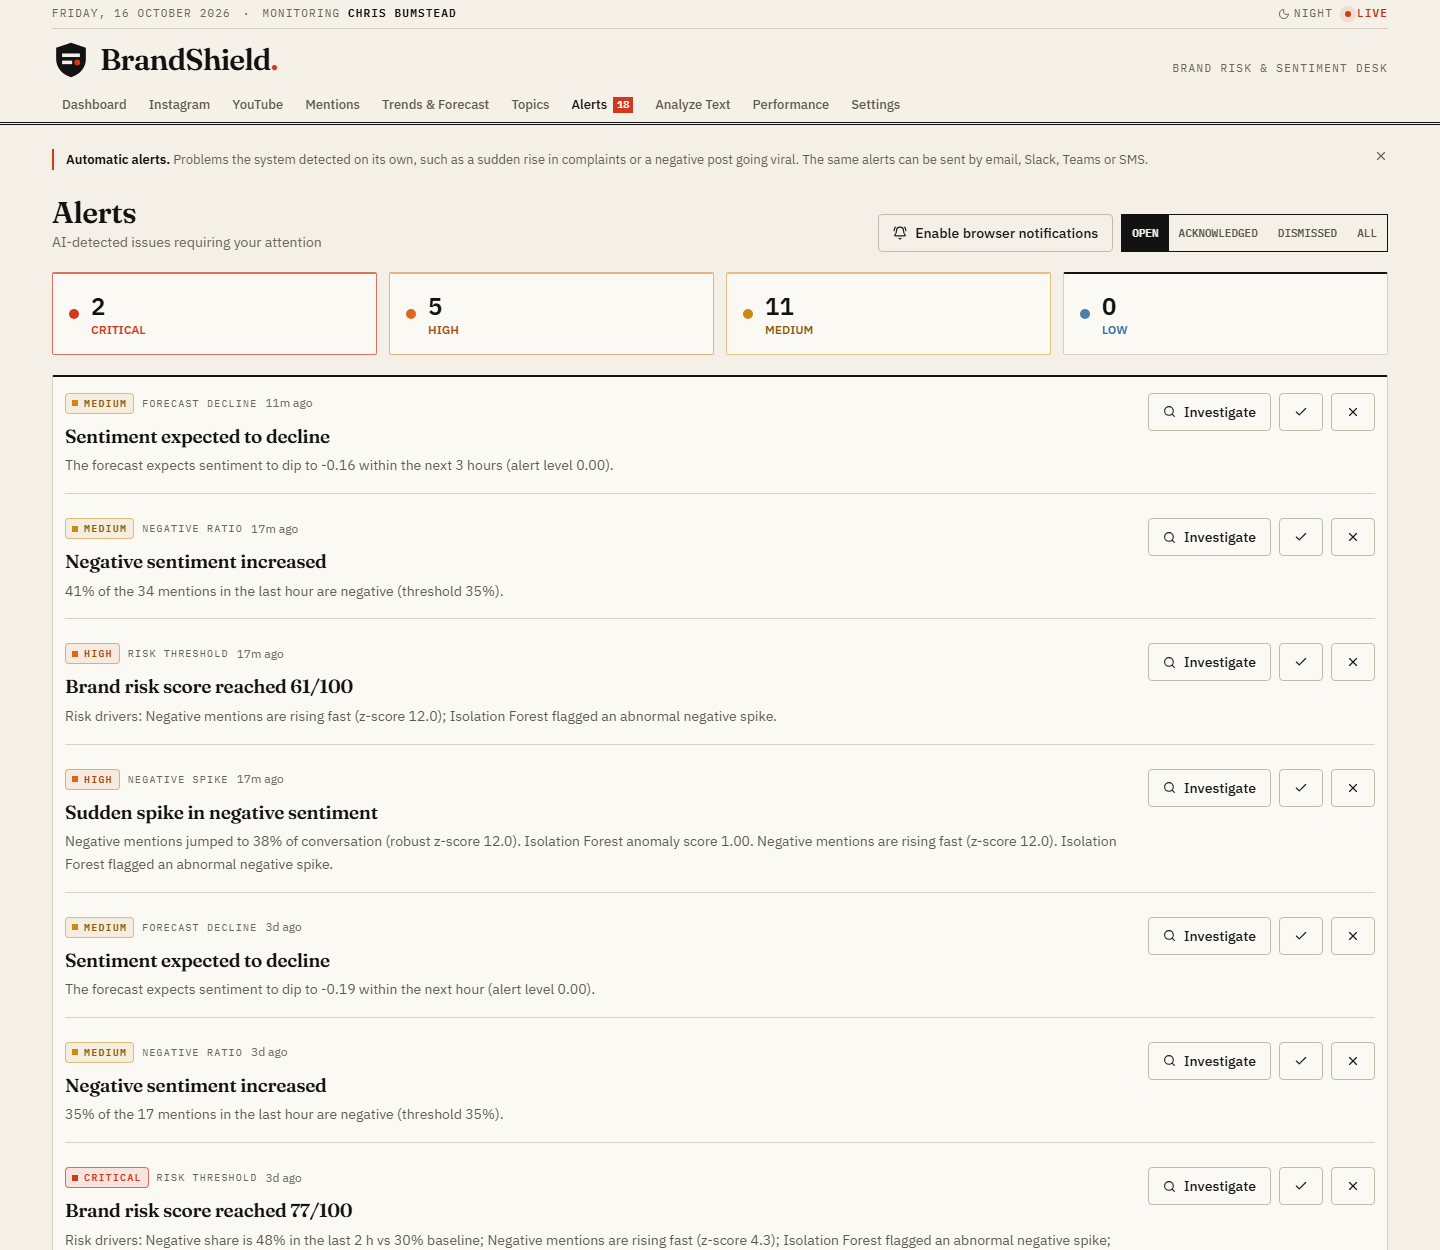
\includegraphics[width=\linewidth,height=0.45\textheight,keepaspectratio]{figures/ui-alerts.png}
\caption{Alerts}
\label{fig:ui-alerts}
\end{figure}

\begin{figure}[!htbp]
\centering
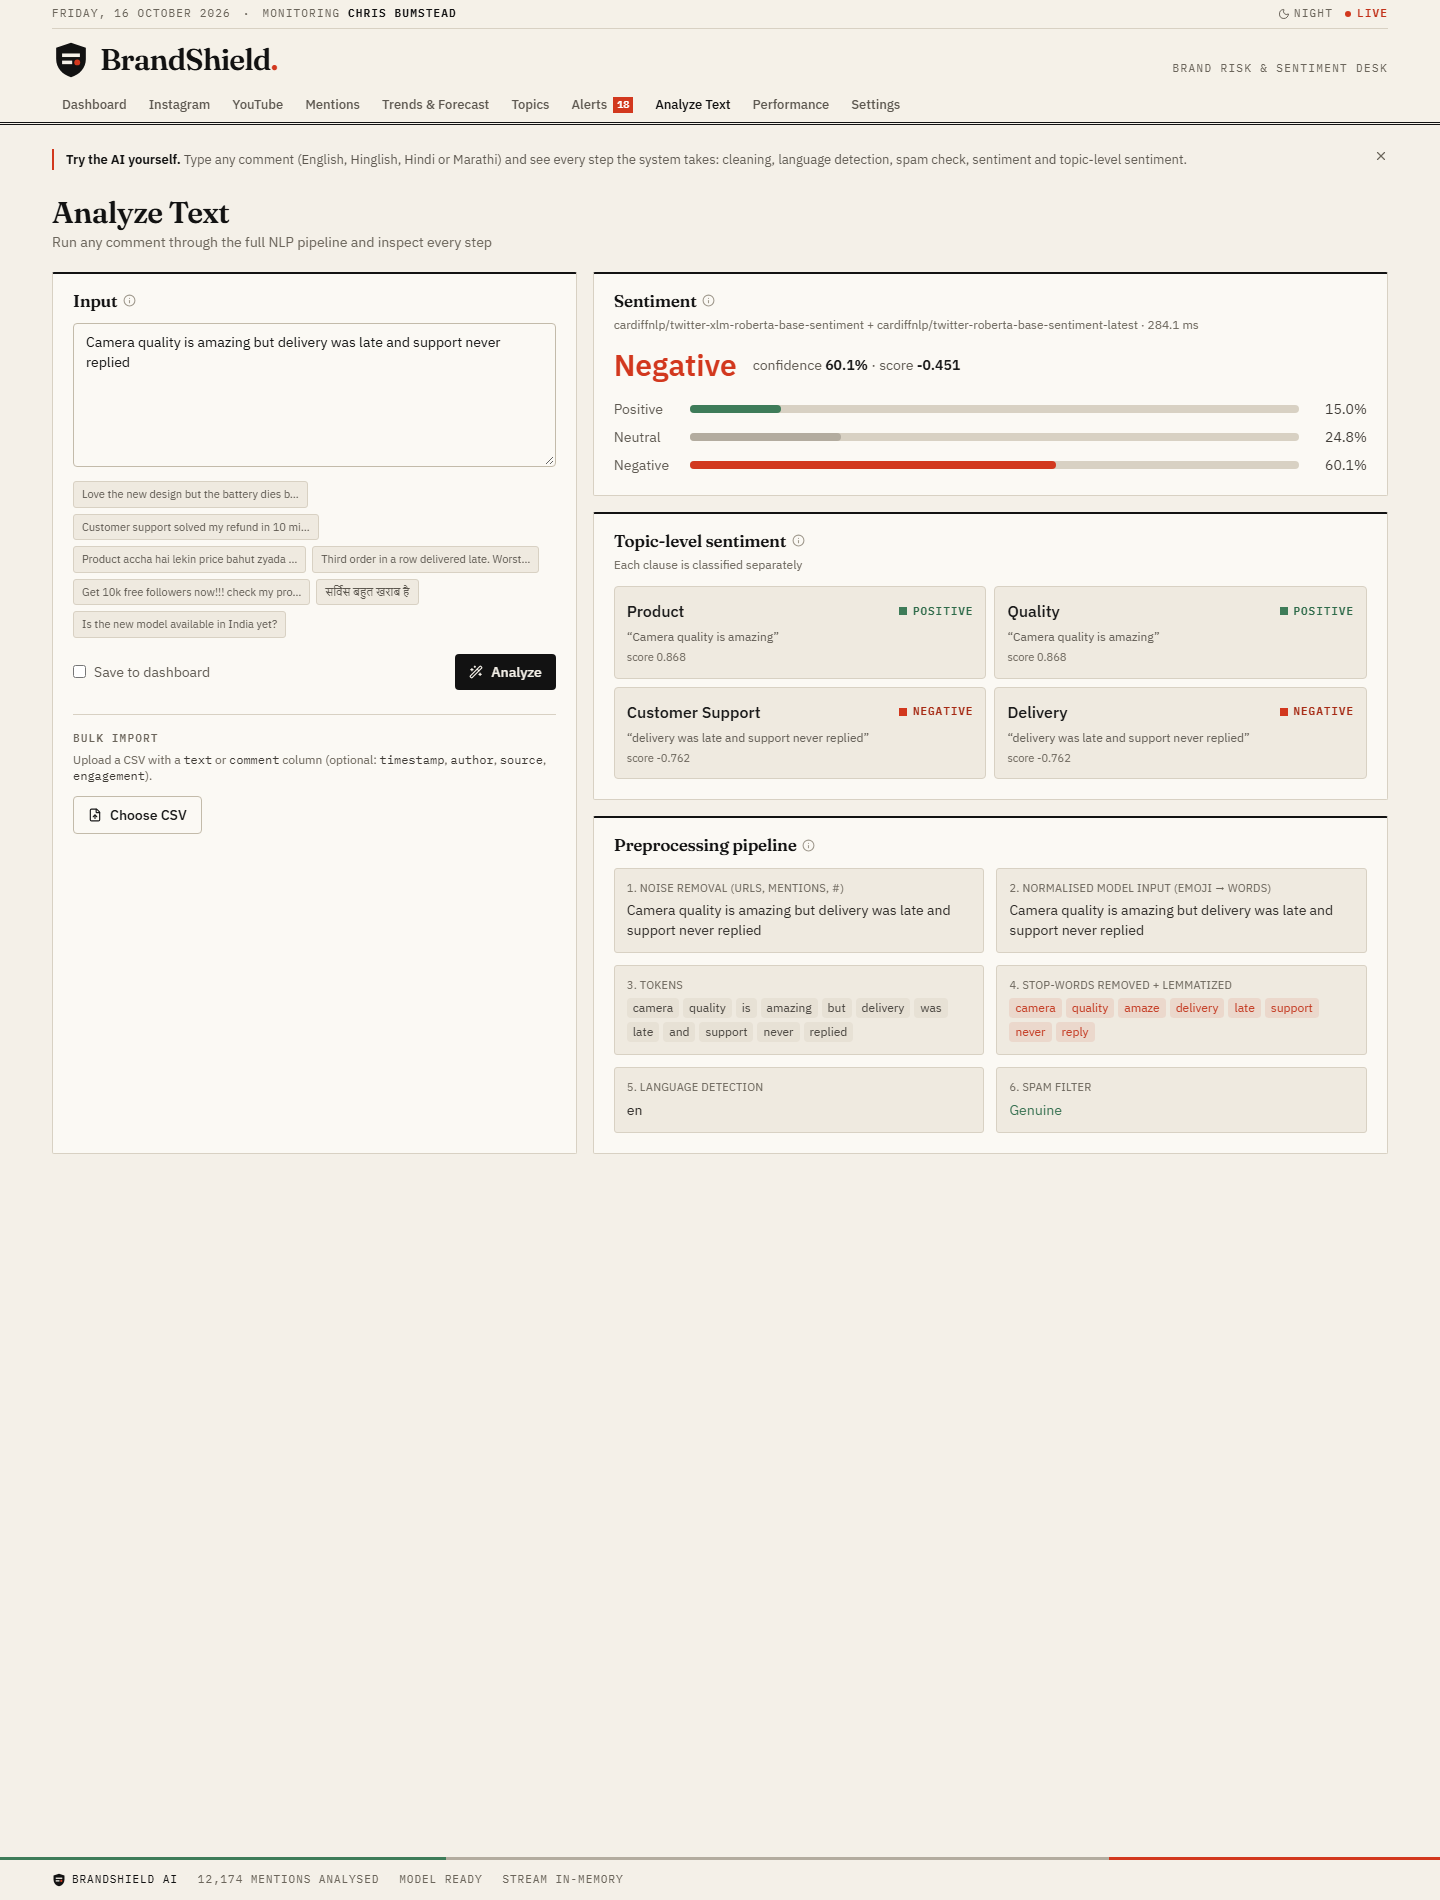
\includegraphics[width=\linewidth,height=0.45\textheight,keepaspectratio]{figures/ui-analyze.png}
\caption{Analyze Text}
\label{fig:ui-analyze}
\end{figure}

\textbf{Analyze Text.} This page was originally built for our own debugging, but it turned out to be the most useful page during reviews. You can paste any comment and see every step: the cleaned text, tokens, detected language, spam check, class probabilities, final label and aspect-wise sentiment.

\begin{figure}[!htbp]
\centering
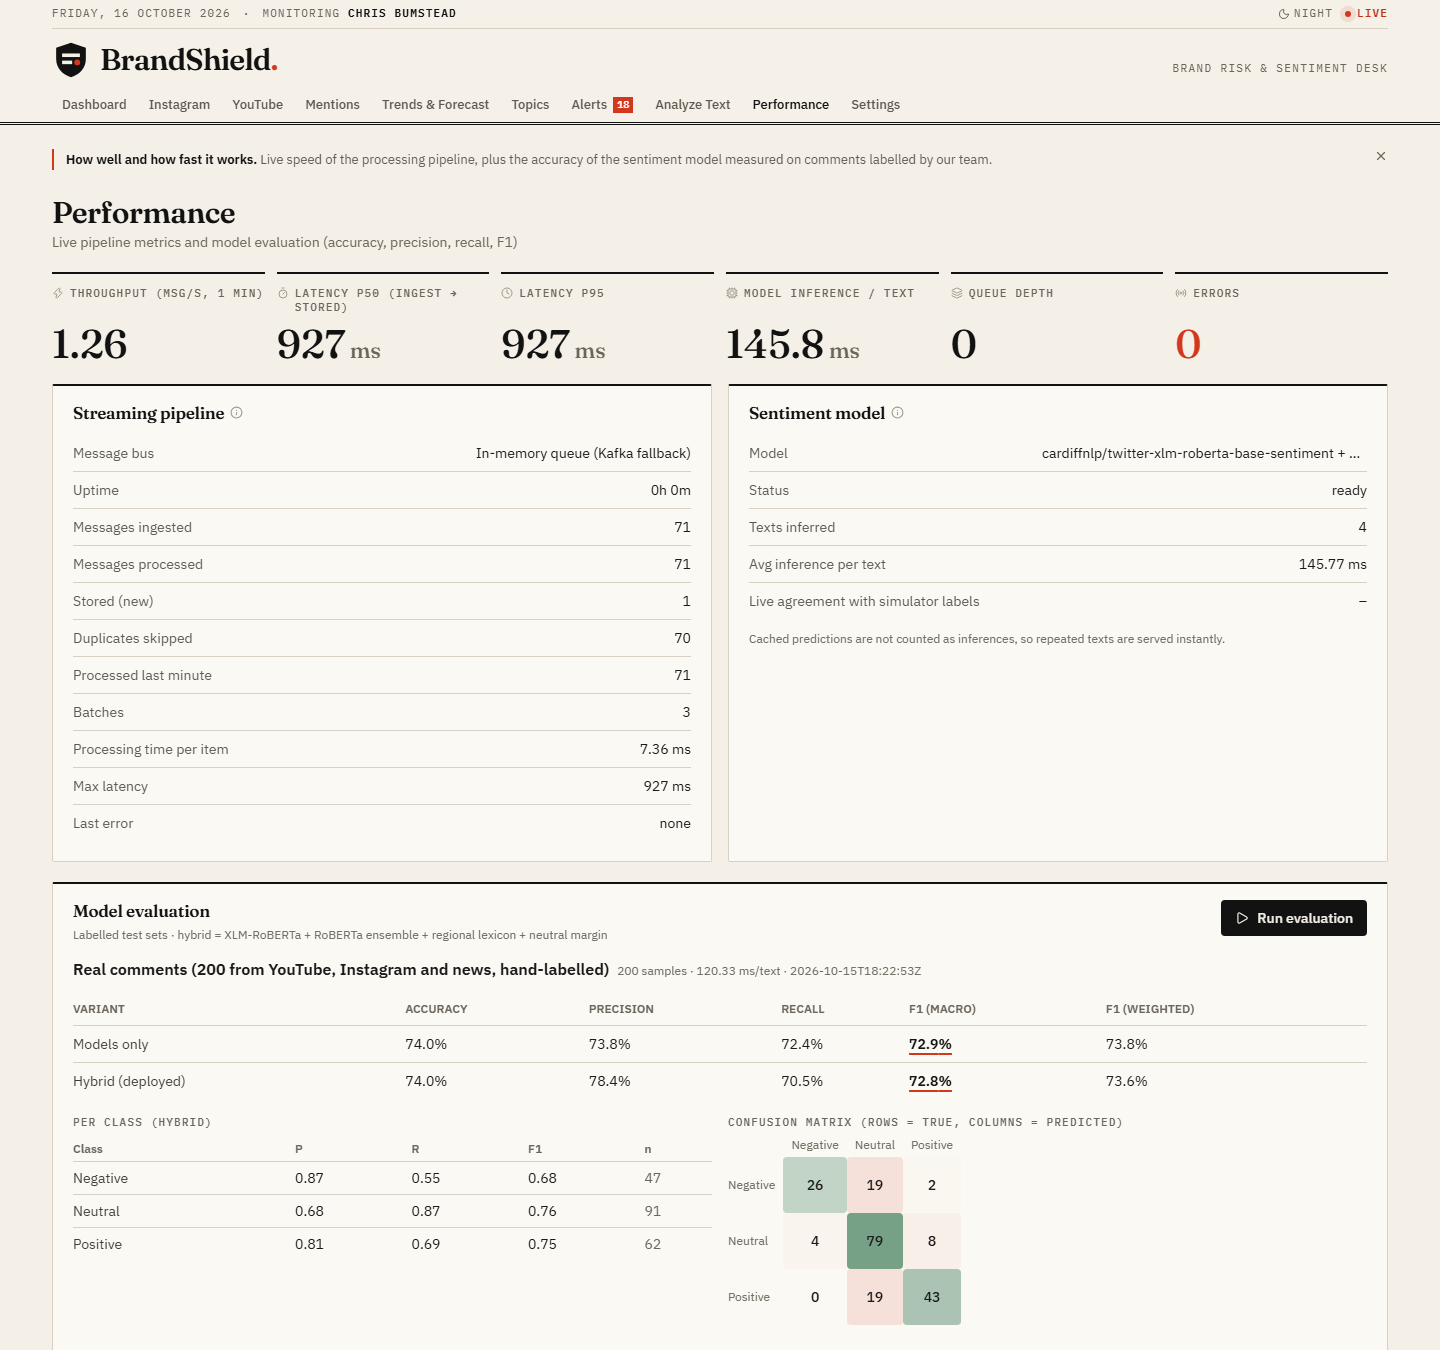
\includegraphics[width=\linewidth,height=0.45\textheight,keepaspectratio]{figures/ui-performance.png}
\caption{System Performance}
\label{fig:ui-system}
\end{figure}

\begin{figure}[!htbp]
\centering
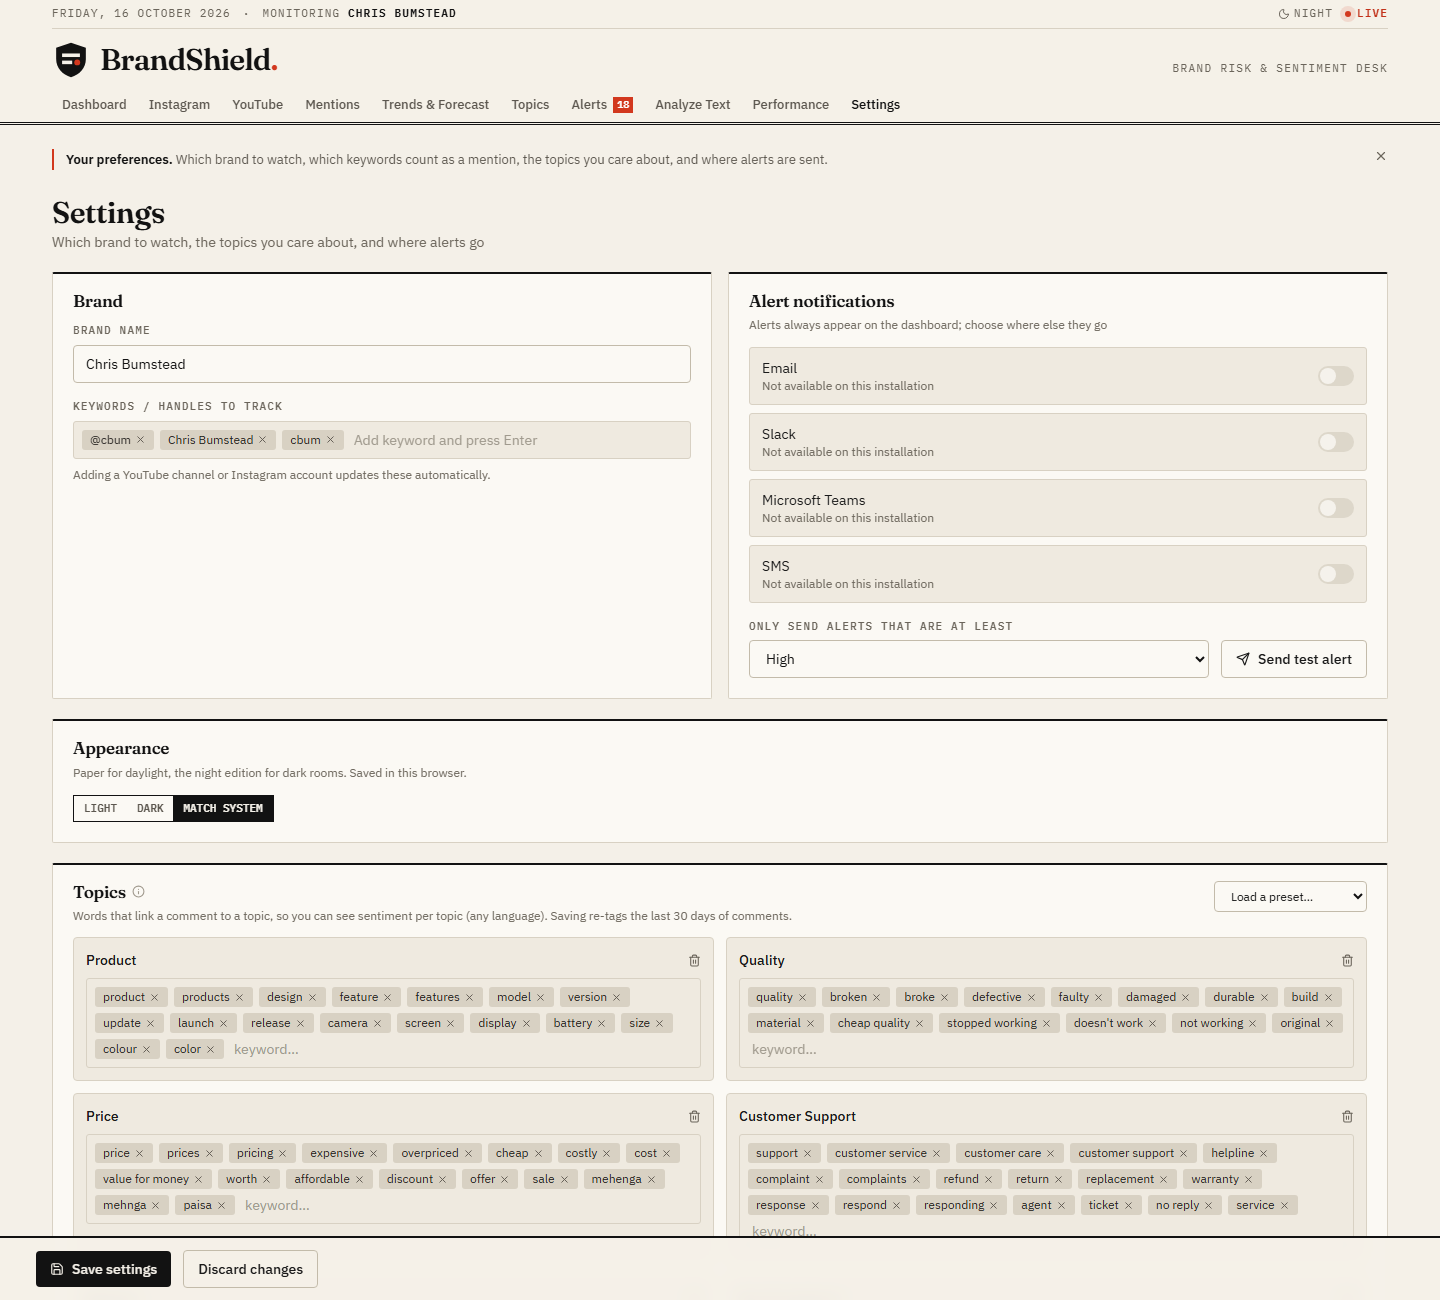
\includegraphics[width=\linewidth,height=0.45\textheight,keepaspectratio]{figures/ui-settings.png}
\caption{Settings}
\label{fig:ui-settings}
\end{figure}

\section{Data design}

\subsection{Data structure}

Inside the program, data moves between modules as a few well-defined structures:

\begin{itemize}
    \item \textbf{Raw mention:} a dictionary produced by a collector with the source, external ID, author, text, URL, creation time and engagement count. This is what goes onto the message bus.
    \item \textbf{Prepared text:} the output of the preprocessor. It holds the cleaned text, the text sent to the model (with emojis converted to words), the tokens, the lemmas, the detected language and the spam flag with its reason.
    \item \textbf{Sentiment result:} the label, confidence, continuous score from $-1$ to $+1$, the three class probabilities, and the lexicon polarity if any code-mixed words were matched.
    \item \textbf{Aspect result:} a list of entries, each with the aspect name, its sentiment, its score and the evidence clause.
    \item \textbf{Time bucket:} a row in a pandas data frame holding, for one 15-minute window, the total count, the count per class, the mean score, the negative share and the anomaly flags.
    \item \textbf{Runtime configuration:} a JSON object holding the brand name, keywords, enabled sources, simulator rate, aspect lexicon, thresholds and notification settings.
\end{itemize}

\subsection{Database Description}

The system uses a single SQLite database with seven tables. Relationships between tables are maintained in code rather than with foreign key constraints, which keeps migrations simple. Figure~\ref{fig:schema} shows the schema and Table~\ref{tab:mentions} describes the main table.

\lofsection{Schema Diagram}
\begin{figure}[!htbp]
\centering
\resizebox{\linewidth}{!}{%
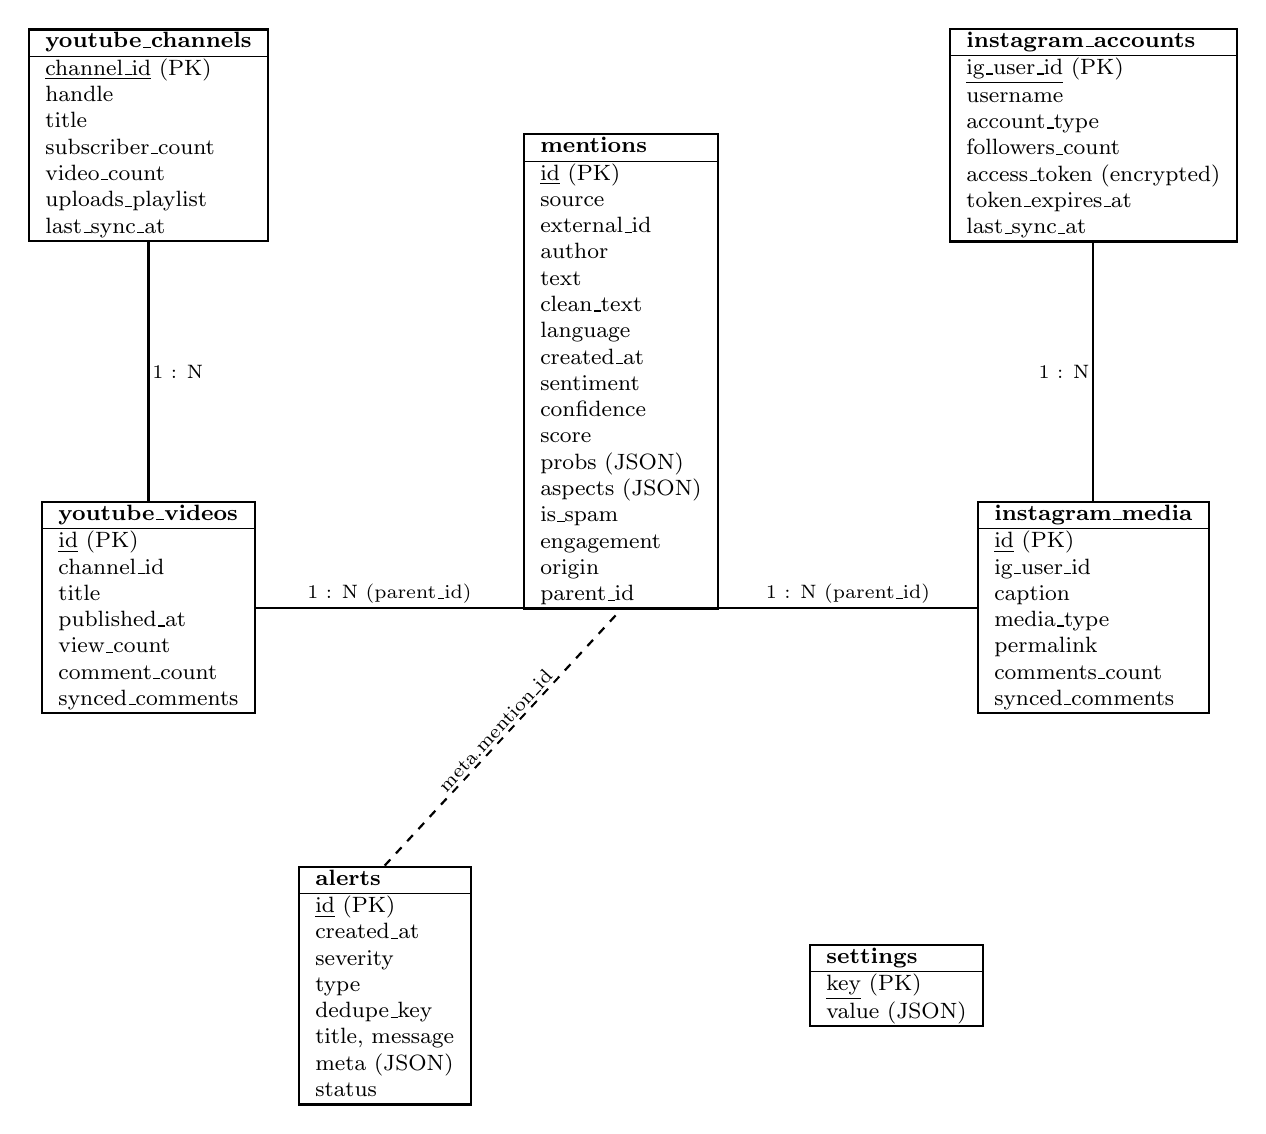
\begin{tikzpicture}[
    tbl/.style={draw, thick, inner sep=0pt, fill=white, font=\footnotesize},
    rel/.style={thick},
    lab/.style={font=\scriptsize, fill=white, inner sep=1pt}]
  \node[tbl] (yc) at (-6,3.6) {\begin{tabular}{l}\textbf{youtube\_channels}\\\hline \underline{channel\_id} (PK)\\handle\\title\\subscriber\_count\\video\_count\\uploads\_playlist\\last\_sync\_at\end{tabular}};
  \node[tbl] (yv) at (-6,-2.4) {\begin{tabular}{l}\textbf{youtube\_videos}\\\hline \underline{id} (PK)\\channel\_id\\title\\published\_at\\view\_count\\comment\_count\\synced\_comments\end{tabular}};
  \node[tbl] (m) at (0,0.6) {\begin{tabular}{l}\textbf{mentions}\\\hline \underline{id} (PK)\\source\\external\_id\\author\\text\\clean\_text\\language\\created\_at\\sentiment\\confidence\\score\\probs (JSON)\\aspects (JSON)\\is\_spam\\engagement\\origin\\parent\_id\end{tabular}};
  \node[tbl] (ia) at (6,3.6) {\begin{tabular}{l}\textbf{instagram\_accounts}\\\hline \underline{ig\_user\_id} (PK)\\username\\account\_type\\followers\_count\\access\_token (encrypted)\\token\_expires\_at\\last\_sync\_at\end{tabular}};
  \node[tbl] (im) at (6,-2.4) {\begin{tabular}{l}\textbf{instagram\_media}\\\hline \underline{id} (PK)\\ig\_user\_id\\caption\\media\_type\\permalink\\comments\_count\\synced\_comments\end{tabular}};
  \node[tbl] (al) at (-3,-7.2) {\begin{tabular}{l}\textbf{alerts}\\\hline \underline{id} (PK)\\created\_at\\severity\\type\\dedupe\_key\\title, message\\meta (JSON)\\status\end{tabular}};
  \node[tbl] (se) at (3.5,-7.2) {\begin{tabular}{l}\textbf{settings}\\\hline \underline{key} (PK)\\value (JSON)\end{tabular}};

  \draw[rel] (yc) -- node[lab, right]{1 : N} (yv);
  \draw[rel] (ia) -- node[lab, left]{1 : N} (im);
  \draw[rel] (yv.east) -- node[lab, above]{1 : N (parent\_id)} (m.west |- yv.east);
  \draw[rel] (im.west) -- node[lab, above]{1 : N (parent\_id)} (m.east |- im.west);
  \draw[rel, dashed] (al.north) -- node[lab, sloped, above]{meta.mention\_id} (m.south);
\end{tikzpicture}}
\caption{Relational Schema Diagram}
\label{fig:schema}
\end{figure}

\begin{longtable}{|P{2.8cm}|P{2.4cm}|P{8.6cm}|}
\caption{Description of the \texttt{mentions} Table}
\label{tab:mentions}\\
\hline
\textbf{Field} & \textbf{Type} & \textbf{Description} \\
\hline
\endfirsthead
\hline
\textbf{Field} & \textbf{Type} & \textbf{Description} \\
\hline
\endhead
id & TEXT (PK) & First 24 characters of SHA-1 of \texttt{source:external\_id}; makes duplicates impossible \\ \hline
source & TEXT & Platform name, e.g. youtube, instagram, rss, appstore \\ \hline
external\_id & TEXT & ID of the comment on the original platform \\ \hline
author & TEXT & Display name or username \\ \hline
text & TEXT & Original comment text \\ \hline
clean\_text & TEXT & Text after preprocessing \\ \hline
language & TEXT & ISO 639-1 language code, or ``unknown'' \\ \hline
created\_at & TEXT & Time the comment was posted (UTC, indexed) \\ \hline
sentiment & TEXT & positive, neutral or negative (indexed) \\ \hline
confidence & REAL & Probability of the chosen class, 0 to 1 \\ \hline
score & REAL & Continuous sentiment score, $-1$ to $+1$ \\ \hline
probs & TEXT (JSON) & Probabilities of all three classes \\ \hline
aspects & TEXT (JSON) & List of aspect, sentiment, score and evidence clause \\ \hline
is\_spam & INTEGER & 1 if flagged as spam, else 0 \\ \hline
spam\_reason & TEXT & Reason for the spam flag \\ \hline
engagement & INTEGER & Likes or reactions, used by the viral-negative rule \\ \hline
true\_label & TEXT & Ground truth where available (e.g. from star ratings) \\ \hline
origin & TEXT & live or simulated \\ \hline
parent\_id & TEXT & ID of the YouTube video or Instagram post \\ \hline
\end{longtable}

The \textbf{alerts} table stores every alert with its severity (low, medium, high, critical), type, de-duplication key, message, delivery status and lifecycle status (open, acknowledged, dismissed). The \textbf{settings} table is a key-value store that holds the runtime configuration as JSON. The four integration tables hold the connected YouTube channels and videos and Instagram accounts and posts.

\section{UML Diagrams}
\vspace{0.1cm}

The UML diagrams below were generated from the actual source code of the system, so they reflect what is implemented rather than an early plan.

\lofsection{UML Diagrams}

\textbf{Use Case Diagram.} Figure~\ref{fig:usecase} shows the four main actors and the use cases each one is involved in. The brand analyst mostly reads and investigates; the operator sets the system up and connects accounts; the evaluator demonstrates and measures the system; and external systems push data in through the API.

\begin{figure}[!htbp]
\centering
\resizebox{\linewidth}{!}{%
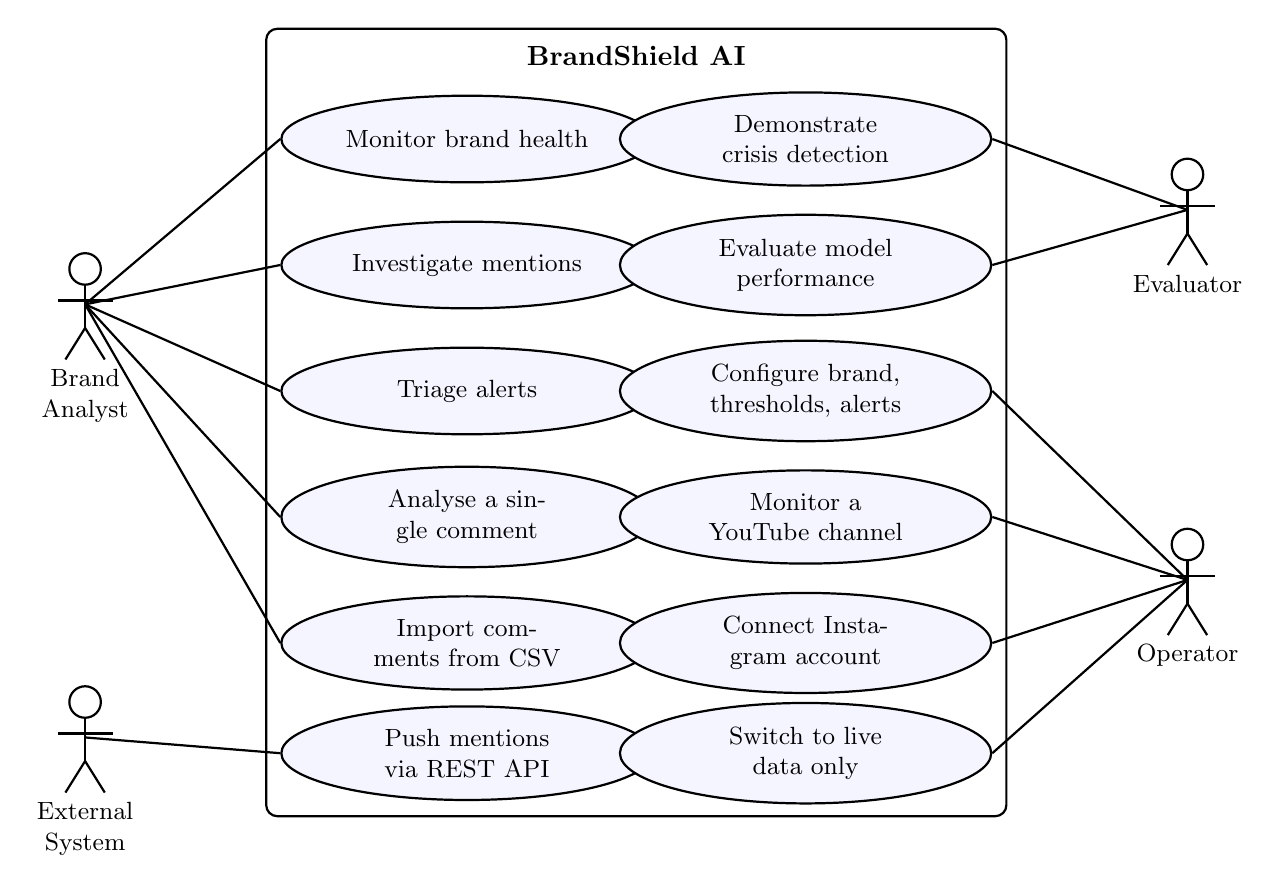
\begin{tikzpicture}[
    uc/.style={draw, thick, ellipse, minimum width=3.9cm, minimum height=1.1cm, align=center, font=\small, fill=blue!4, text width=3.1cm},
    line/.style={thick}]
  \draw[thick, rounded corners] (2.3,1.6) rectangle (11.7,-8.4);
  \node[font=\bfseries] at (7,1.25) {BrandShield AI};

  \node[uc] (u1) at (4.85,0.2) {Monitor brand health};
  \node[uc] (u2) at (4.85,-1.4) {Investigate mentions};
  \node[uc] (u3) at (4.85,-3.0) {Triage alerts};
  \node[uc] (u4) at (4.85,-4.6) {Analyse a single comment};
  \node[uc] (u5) at (4.85,-6.2) {Import comments from CSV};
  \node[uc] (u6) at (4.85,-7.6) {Push mentions via REST API};

  \node[uc] (v1) at (9.15,0.2) {Demonstrate crisis detection};
  \node[uc] (v2) at (9.15,-1.4) {Evaluate model performance};
  \node[uc] (v3) at (9.15,-3.0) {Configure brand, thresholds, alerts};
  \node[uc] (v4) at (9.15,-4.6) {Monitor a YouTube channel};
  \node[uc] (v5) at (9.15,-6.2) {Connect Instagram account};
  \node[uc] (v6) at (9.15,-7.6) {Switch to live data only};

  \actor{an}{0}{-2.4}{Brand\\Analyst}
  \actor{ex}{0}{-7.9}{External\\System}
  \actor{ev}{14}{-1.2}{Evaluator}
  \actor{op}{14}{-5.9}{Operator}

  \foreach \u in {u1,u2,u3,u4,u5} { \draw[line] (an) -- (\u.west); }
  \draw[line] (ex) -- (u6.west);
  \foreach \v in {v1,v2} { \draw[line] (ev) -- (\v.east); }
  \foreach \v in {v3,v4,v5,v6} { \draw[line] (op) -- (\v.east); }
\end{tikzpicture}}
\caption{Use Case Diagram}
\label{fig:usecase}
\end{figure}

\textbf{Class Diagram.} Figure~\ref{fig:class} shows the 28 main classes of the backend. The \texttt{App} class owns every service. All collectors realise the common \texttt{Collector} interface, and both \texttt{MemoryBus} and \texttt{KafkaBus} implement \texttt{MessageBus}, which is why either can be used without changing the rest of the code. The \texttt{Processor} depends on \texttt{TextPreprocessor}, \texttt{SentimentModel} and \texttt{AspectExtractor}, and the \texttt{AnalyticsService} uses \texttt{AnomalyDetector}, \texttt{Forecaster} and \texttt{RiskScorer}.

\begin{figure}[!htbp]
\centering
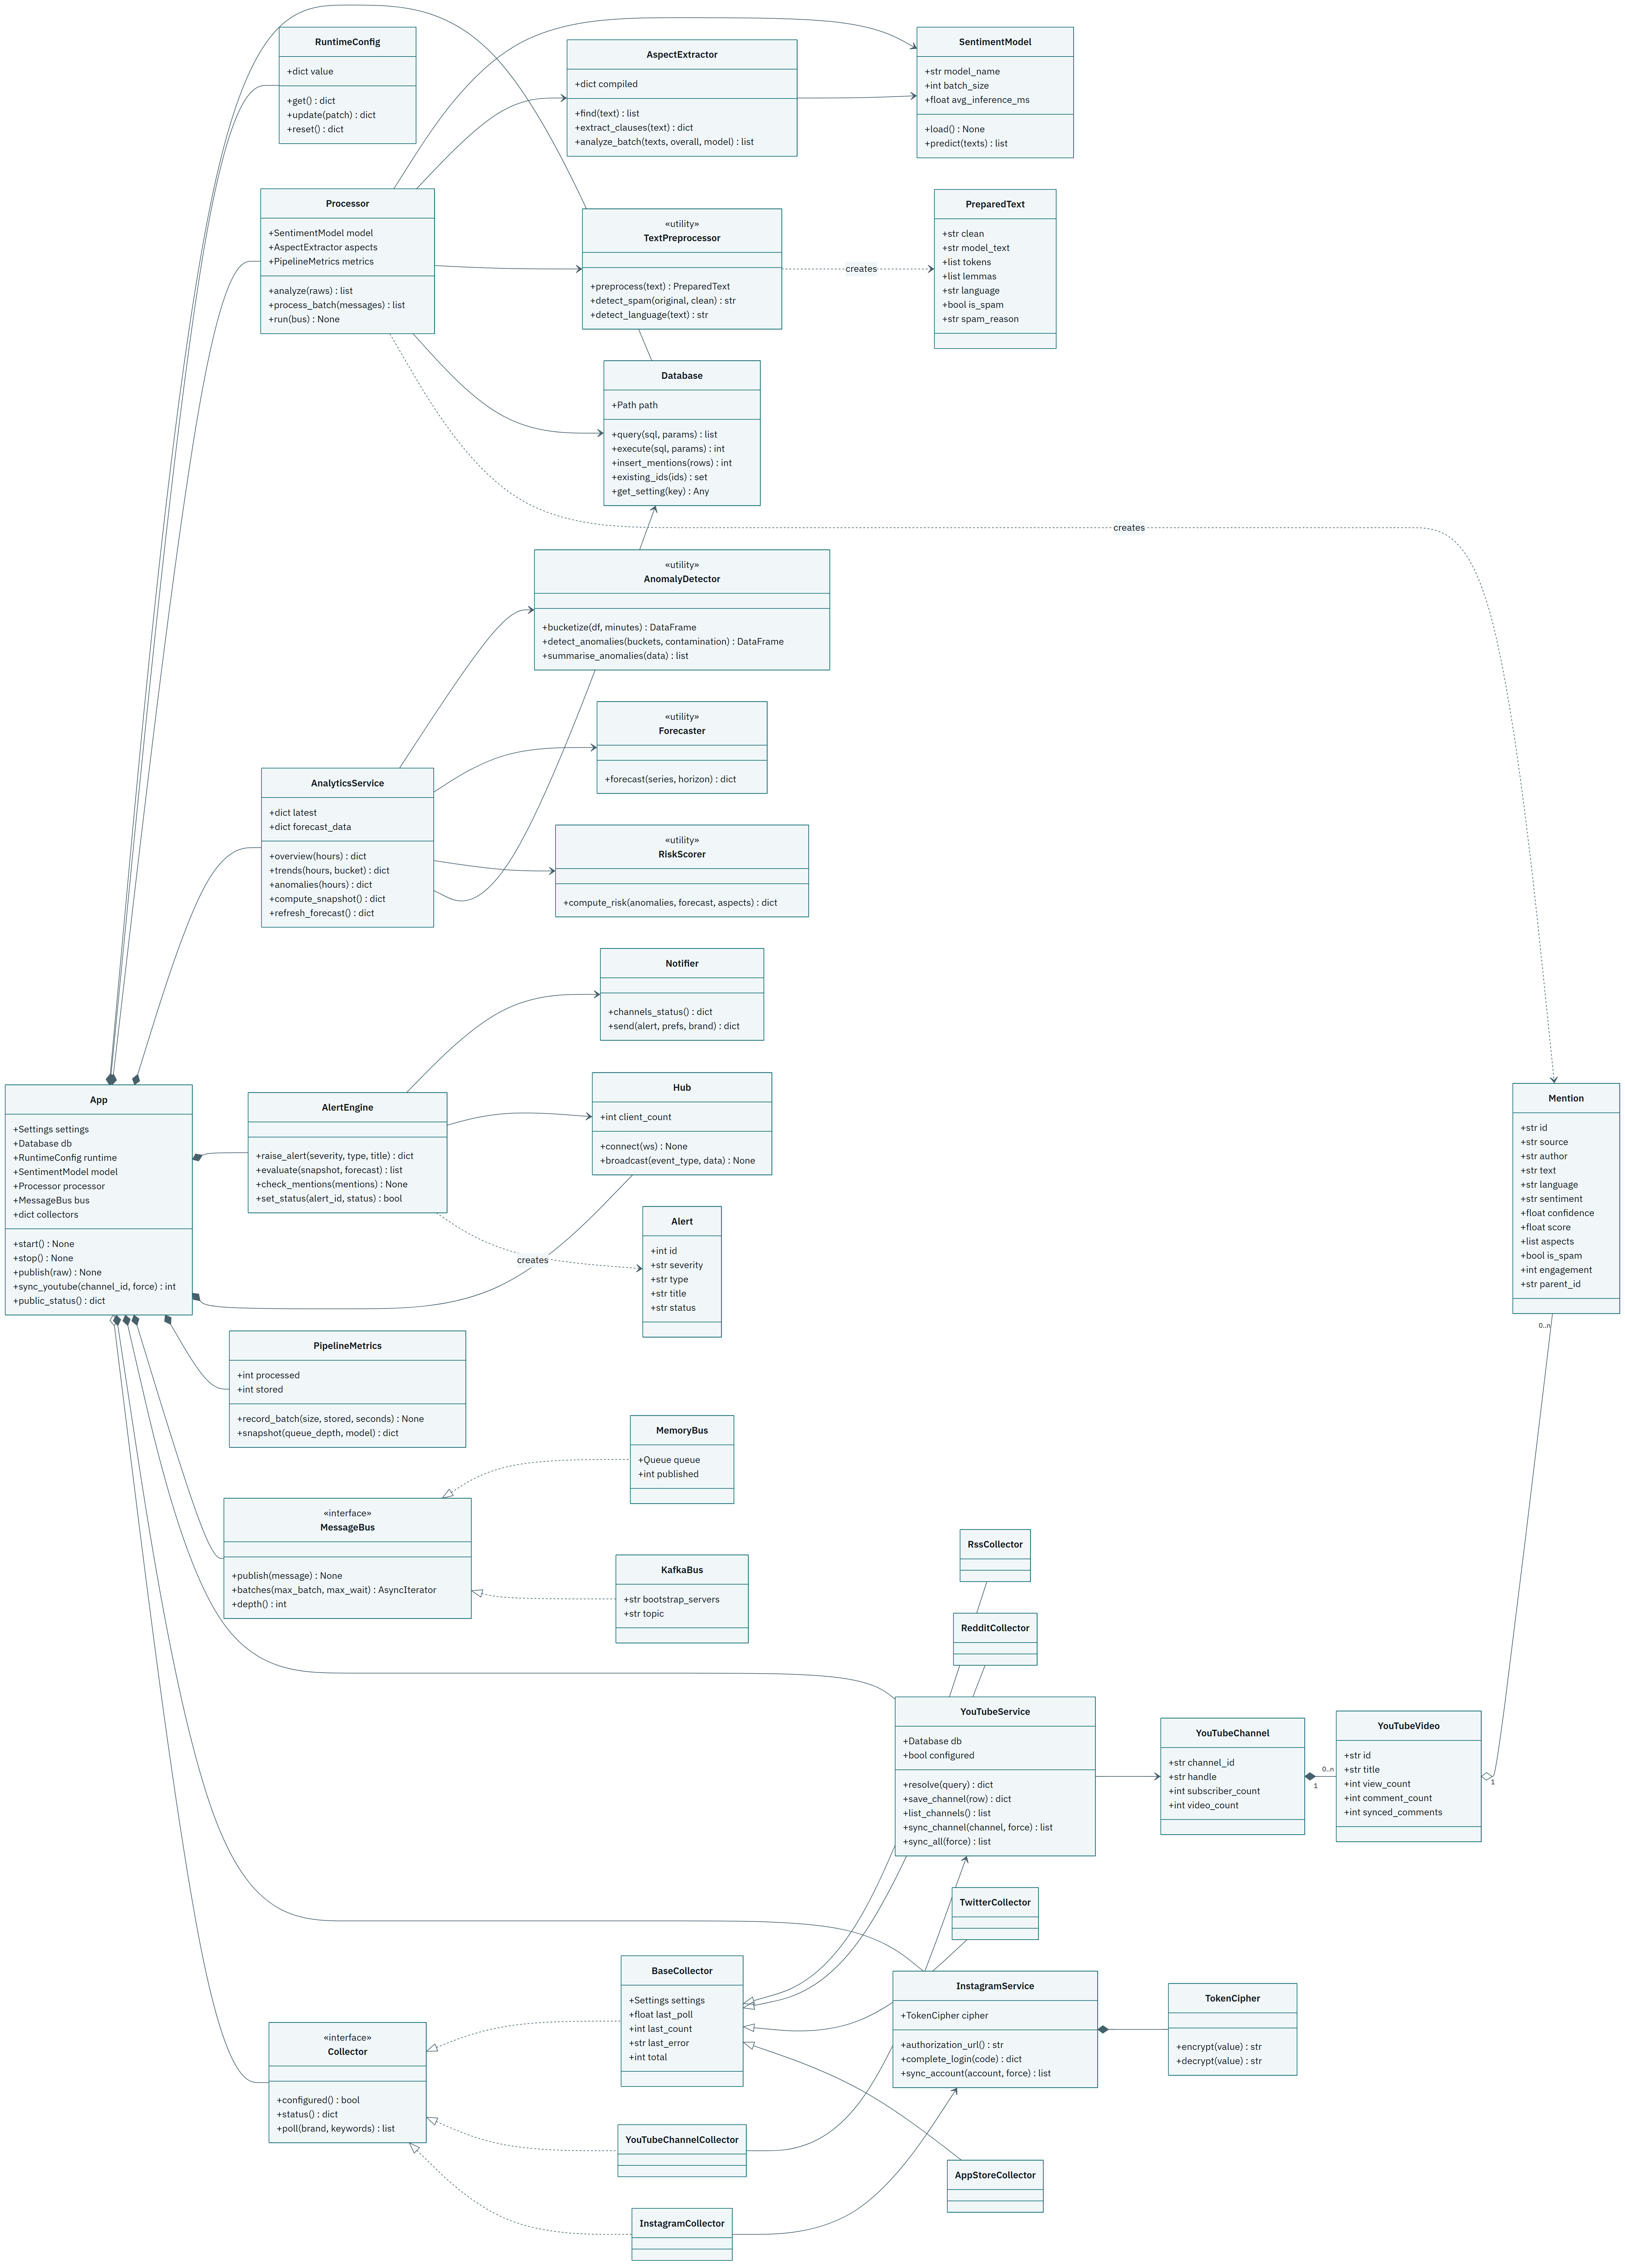
\includegraphics[width=\linewidth, height=17.5cm, keepaspectratio]{figures/01-class-diagram.png}
\caption{Class Diagram (complete)}
\label{fig:class}
\end{figure}

Because the complete diagram is large, Figures~\ref{fig:class-core} and \ref{fig:class-sources} show it split into two readable halves: the core processing pipeline, and the data sources with the analytics classes.

\begin{figure}[!htbp]
\centering
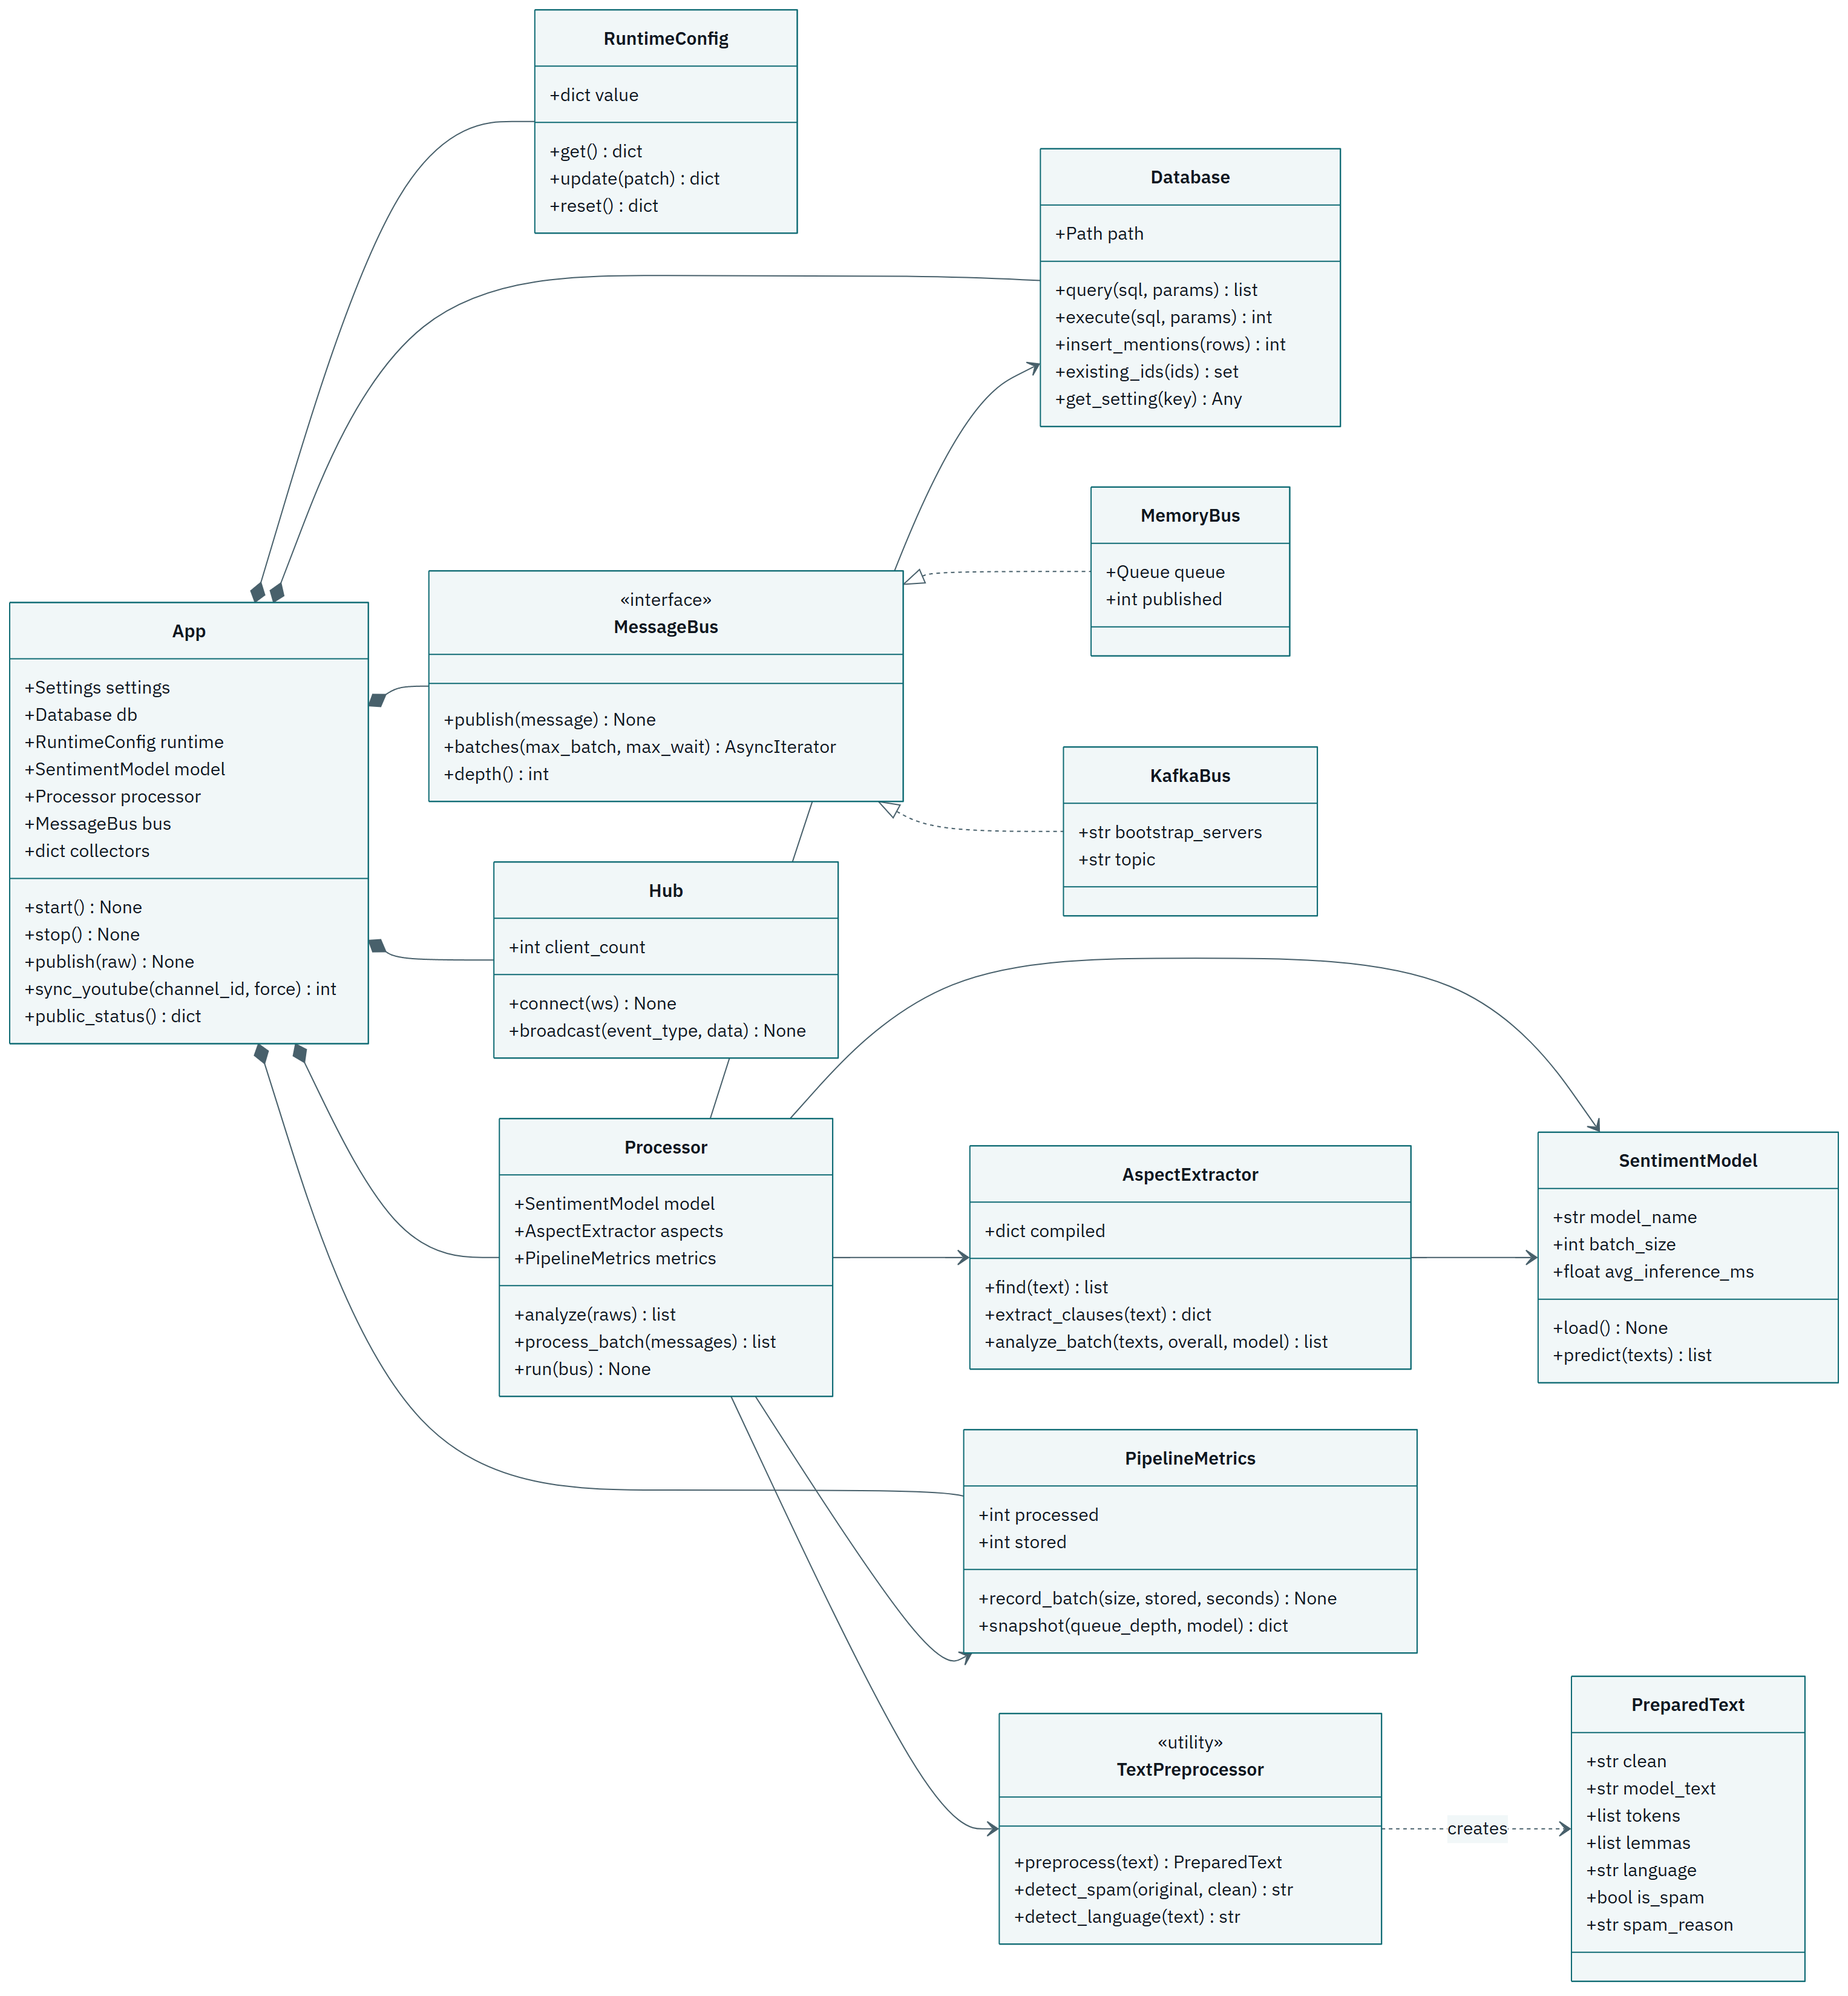
\includegraphics[width=\linewidth, height=17cm, keepaspectratio]{figures/01a-class-core-pipeline.png}
\caption{Class Diagram - Core Pipeline (App, Storage, Message Bus, NLP)}
\label{fig:class-core}
\end{figure}

\begin{figure}[!htbp]
\centering
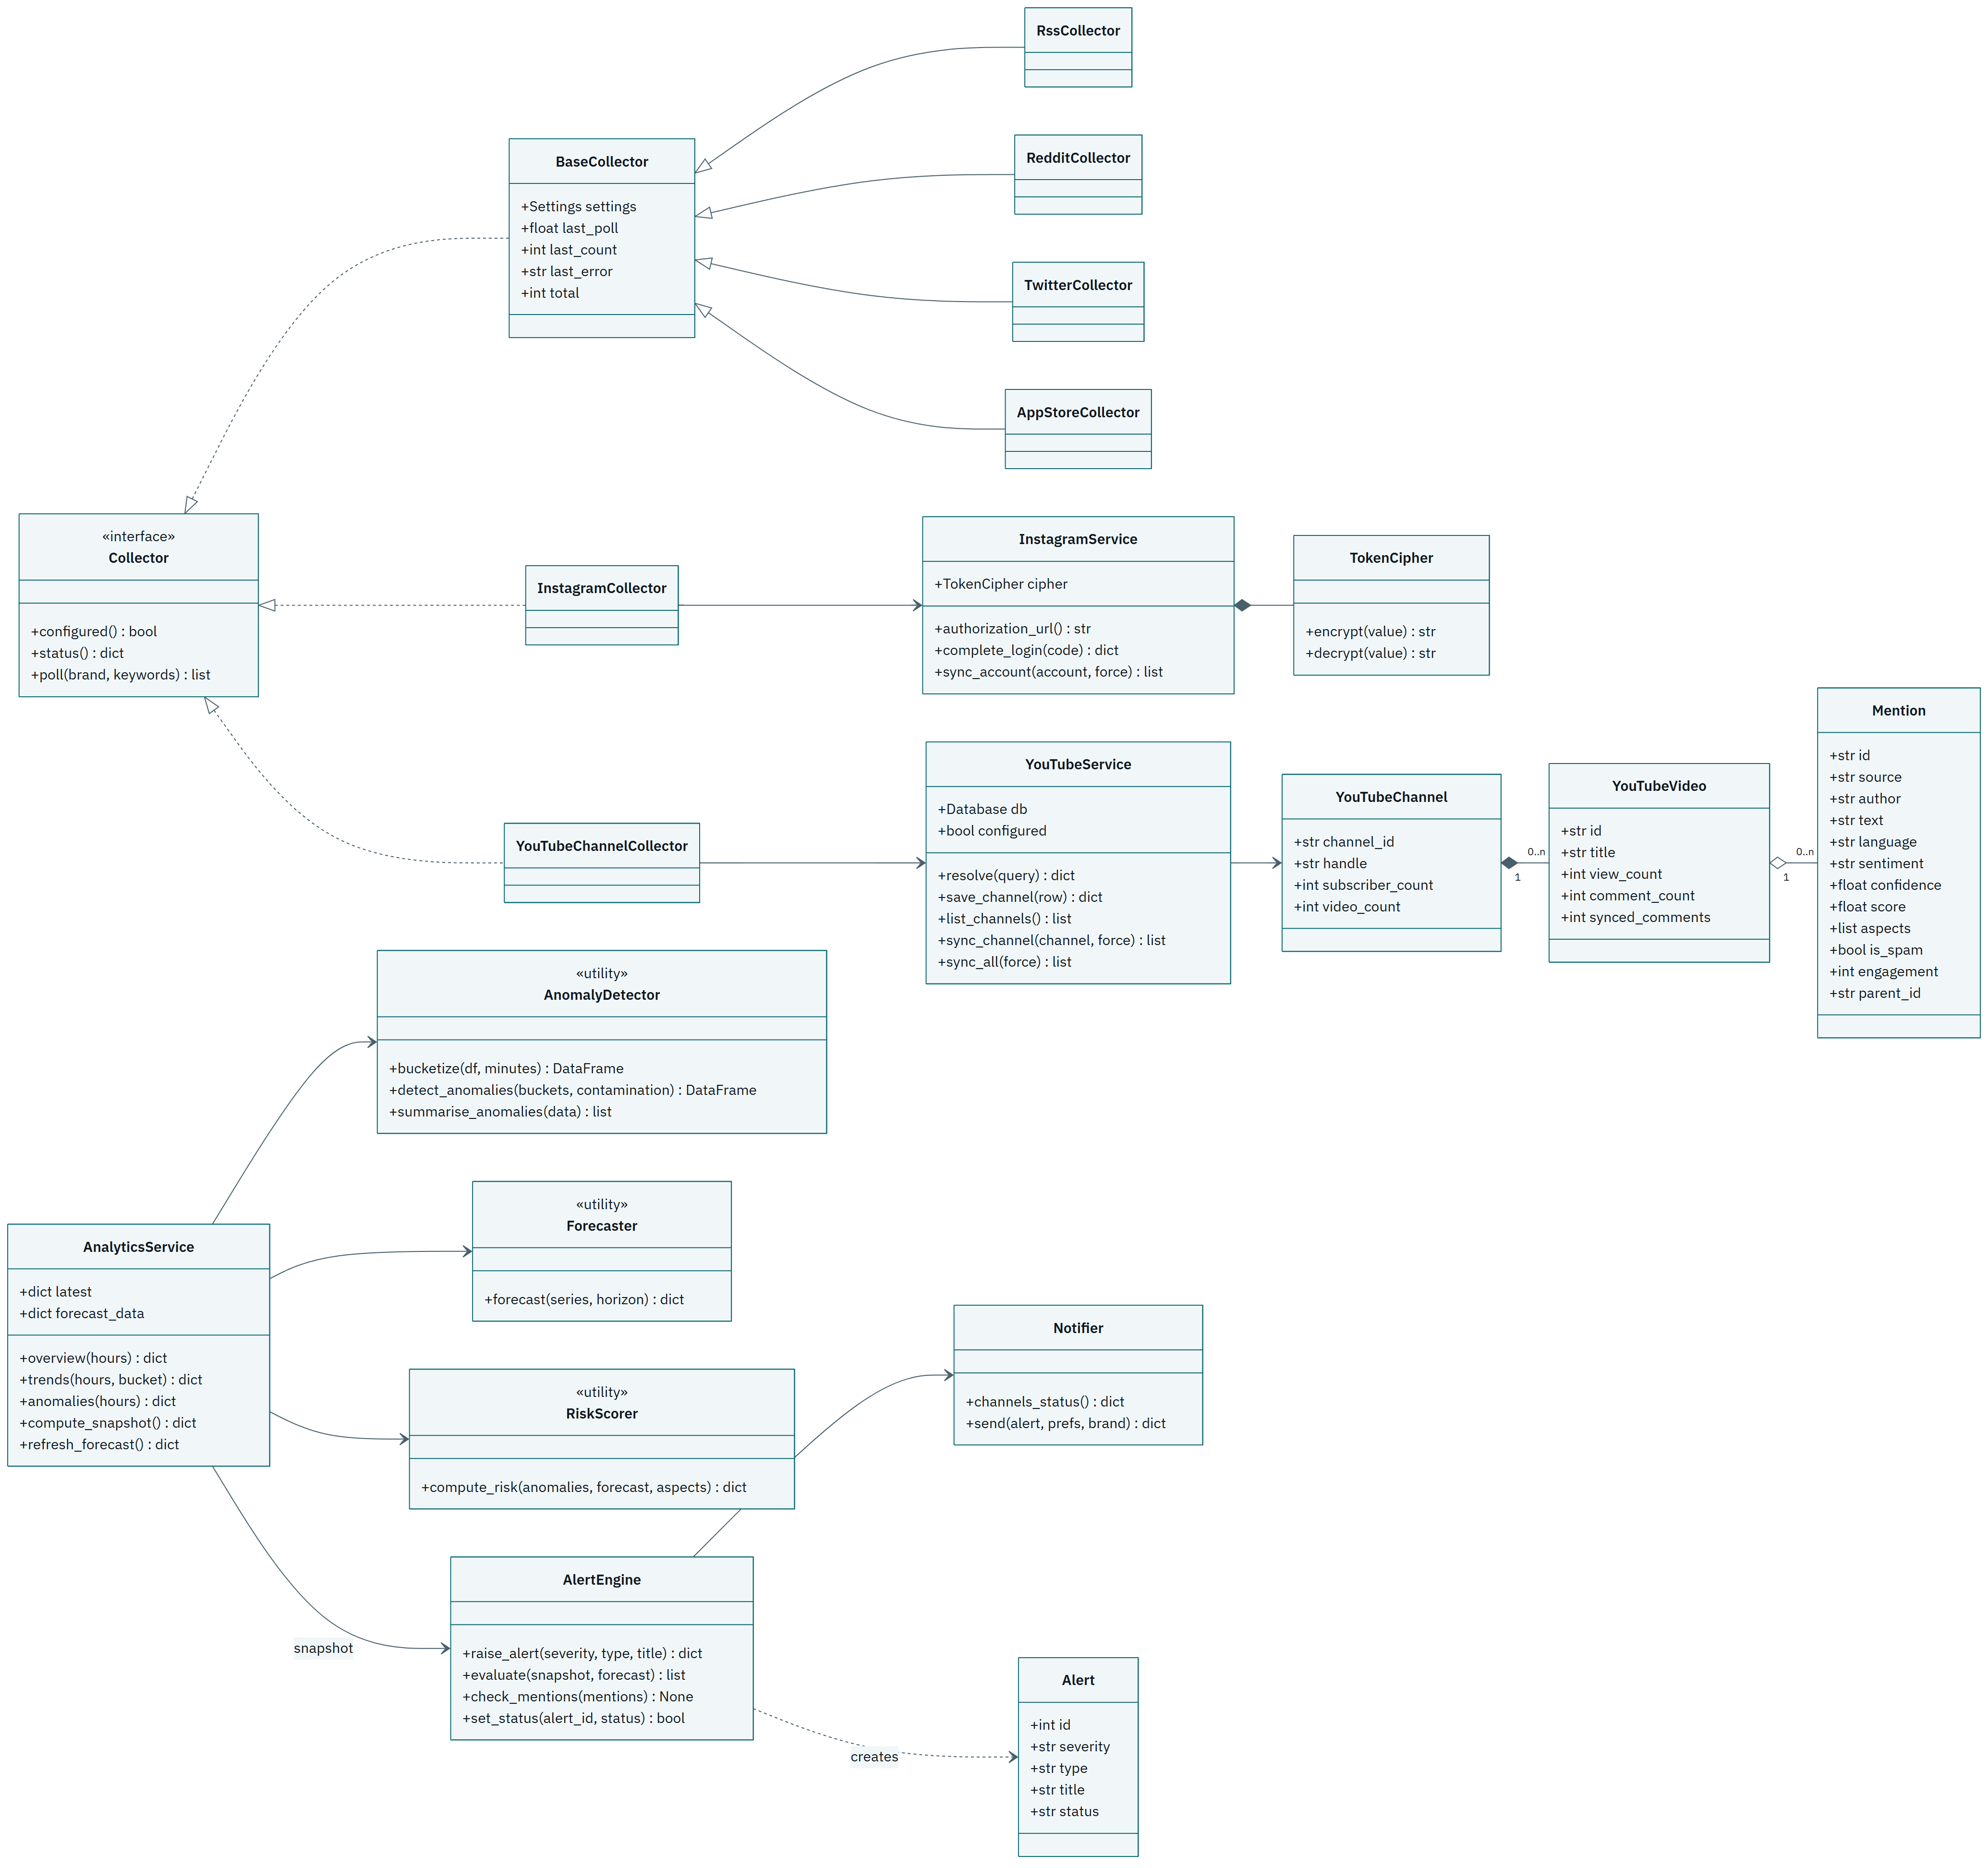
\includegraphics[width=\linewidth, height=17cm, keepaspectratio]{figures/01b-class-sources-analytics.png}
\caption{Class Diagram - Collectors, Services and Analytics}
\label{fig:class-sources}
\end{figure}

\textbf{Class Diagram for Social Integrations.} Figure~\ref{fig:class-social} focuses on the two social media integrations. It shows how the YouTube and Instagram collectors realise the shared \texttt{Collector} interface, which services call each platform API, which entities are stored, and how both end up producing \texttt{Mention} objects for the processing pipeline.

\begin{figure}[!htbp]
\centering
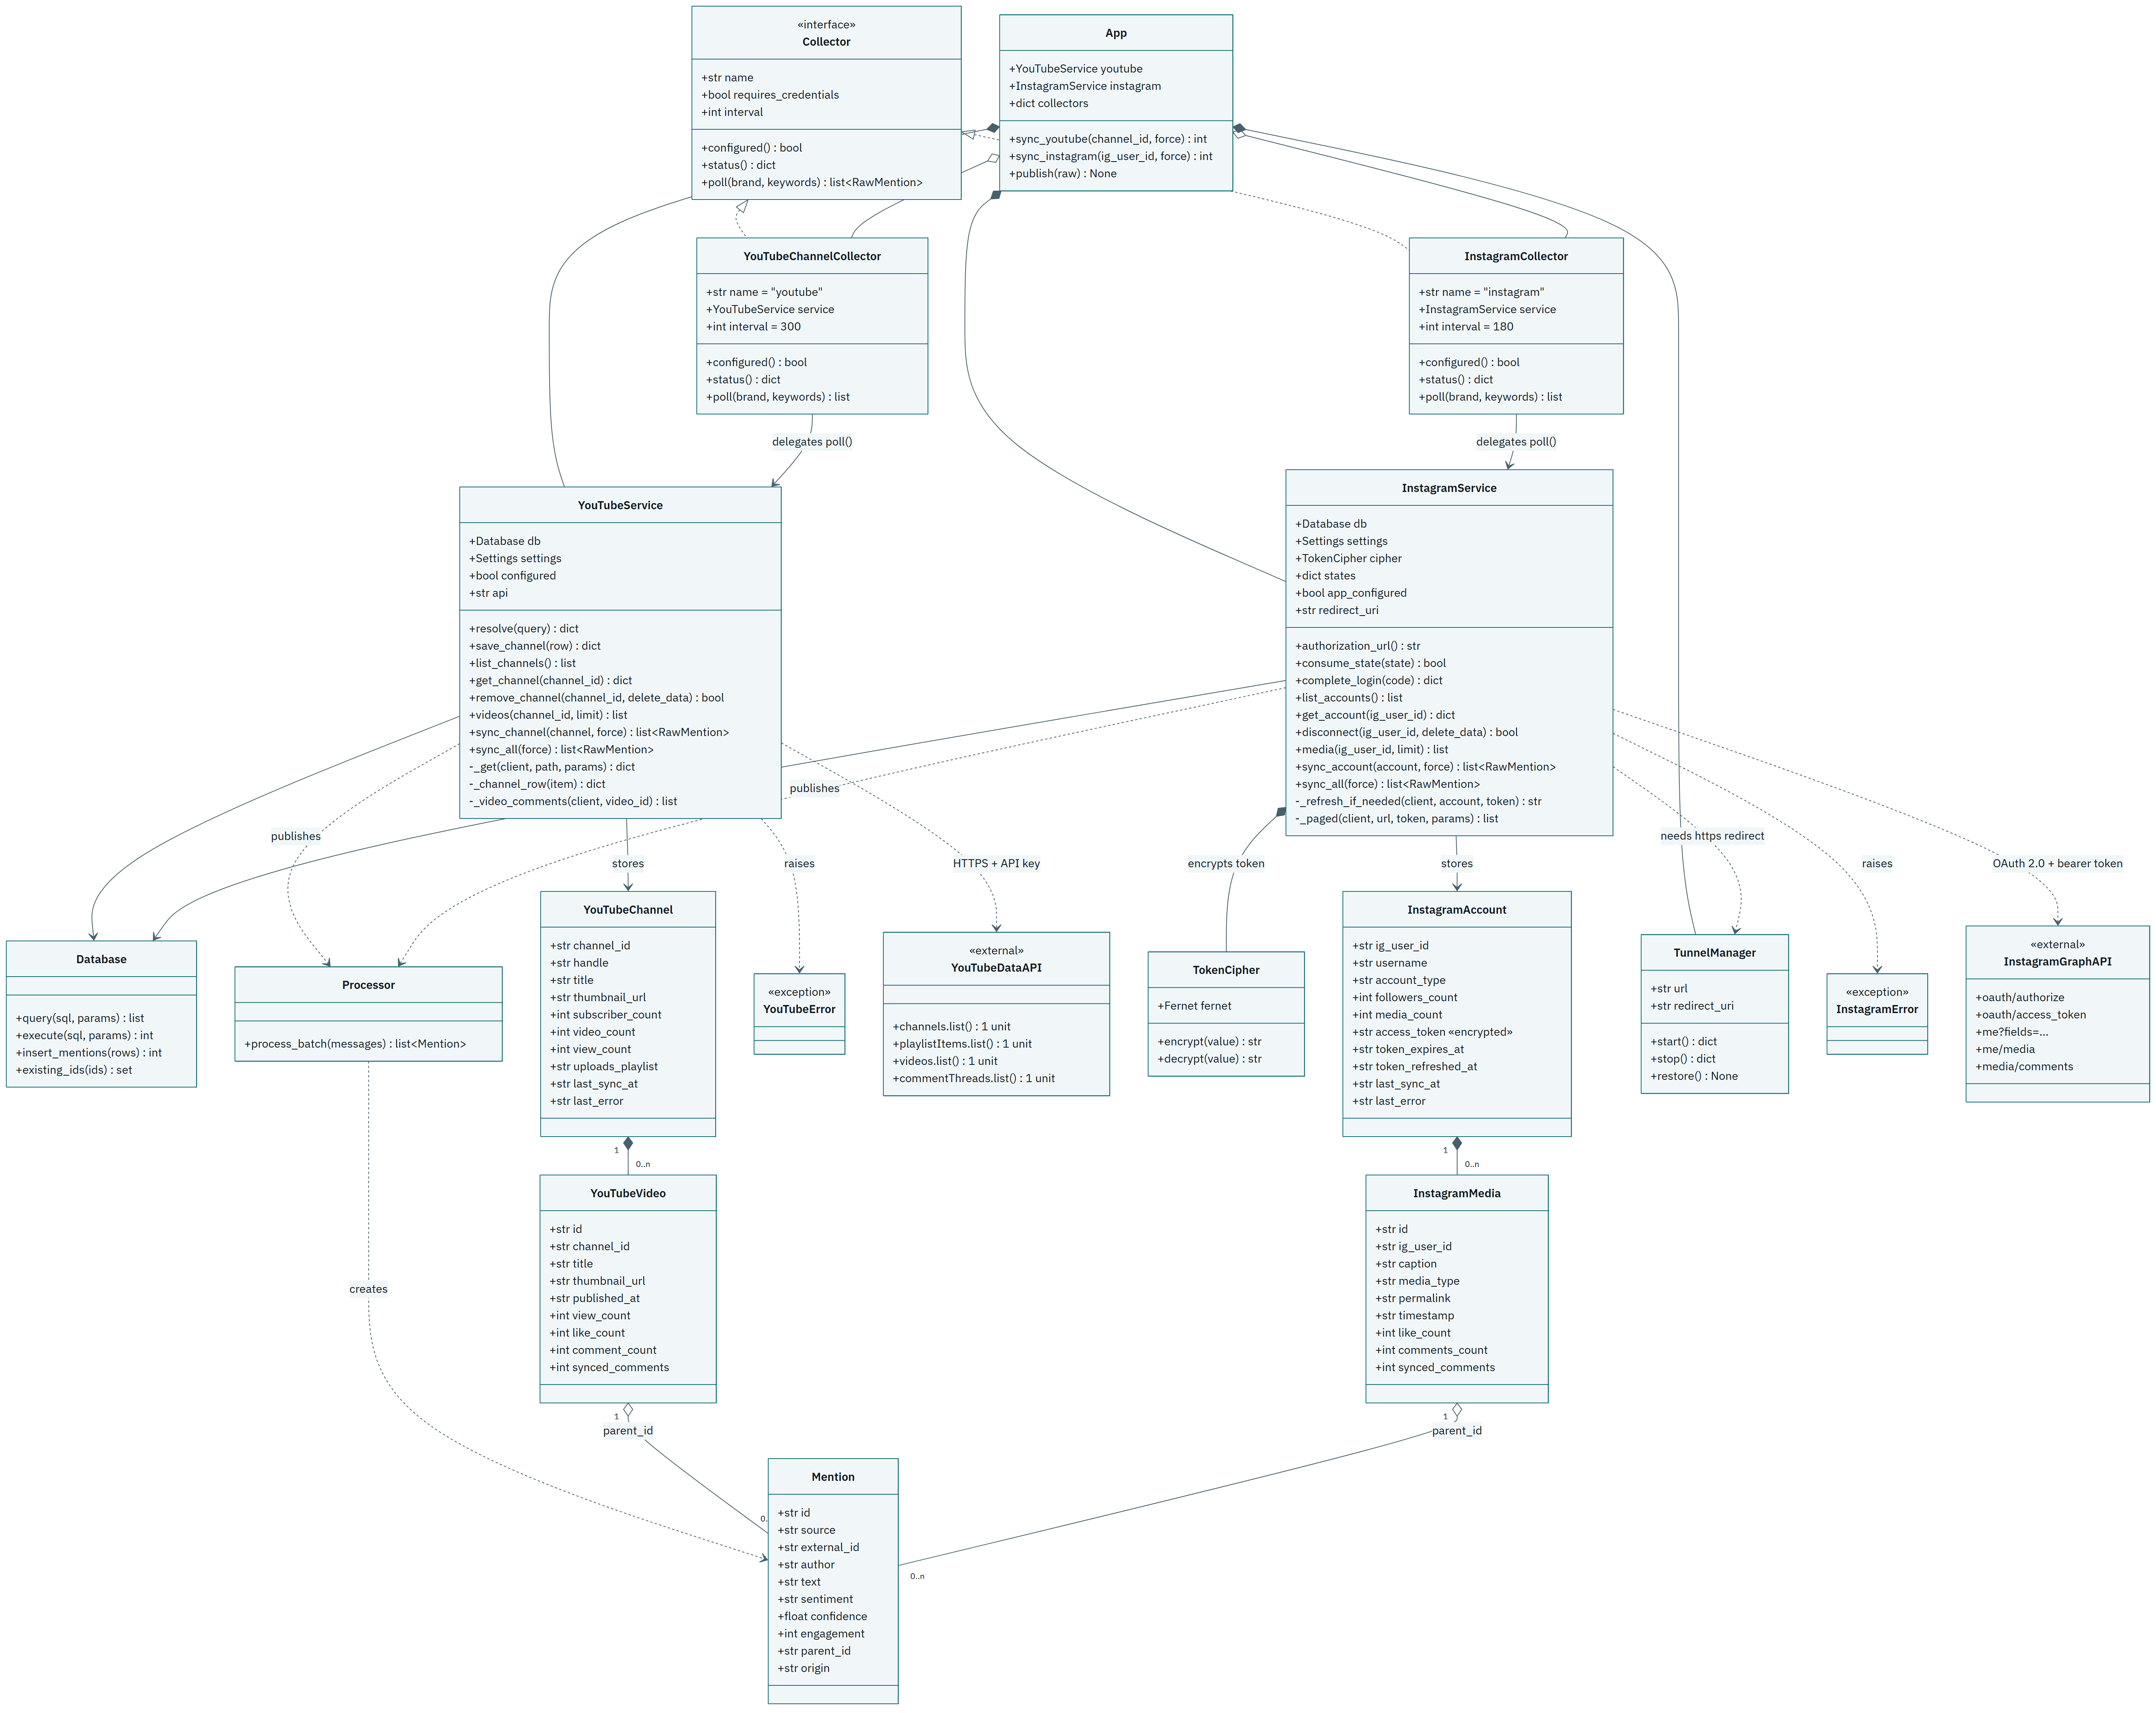
\includegraphics[width=\linewidth, height=17cm, keepaspectratio]{figures/04-class-diagram-social-integrations.png}
\caption{Class Diagram - YouTube and Instagram Integrations}
\label{fig:class-social}
\end{figure}

\textbf{Object Diagram.} Figure~\ref{fig:object} is a snapshot of the running system, taken while it was monitoring a public YouTube channel. The values are real: at that moment the application held 9,984 analysed mentions, was using the in-memory bus, and had the sentiment model loaded and ready.

\begin{figure}[!htbp]
\centering
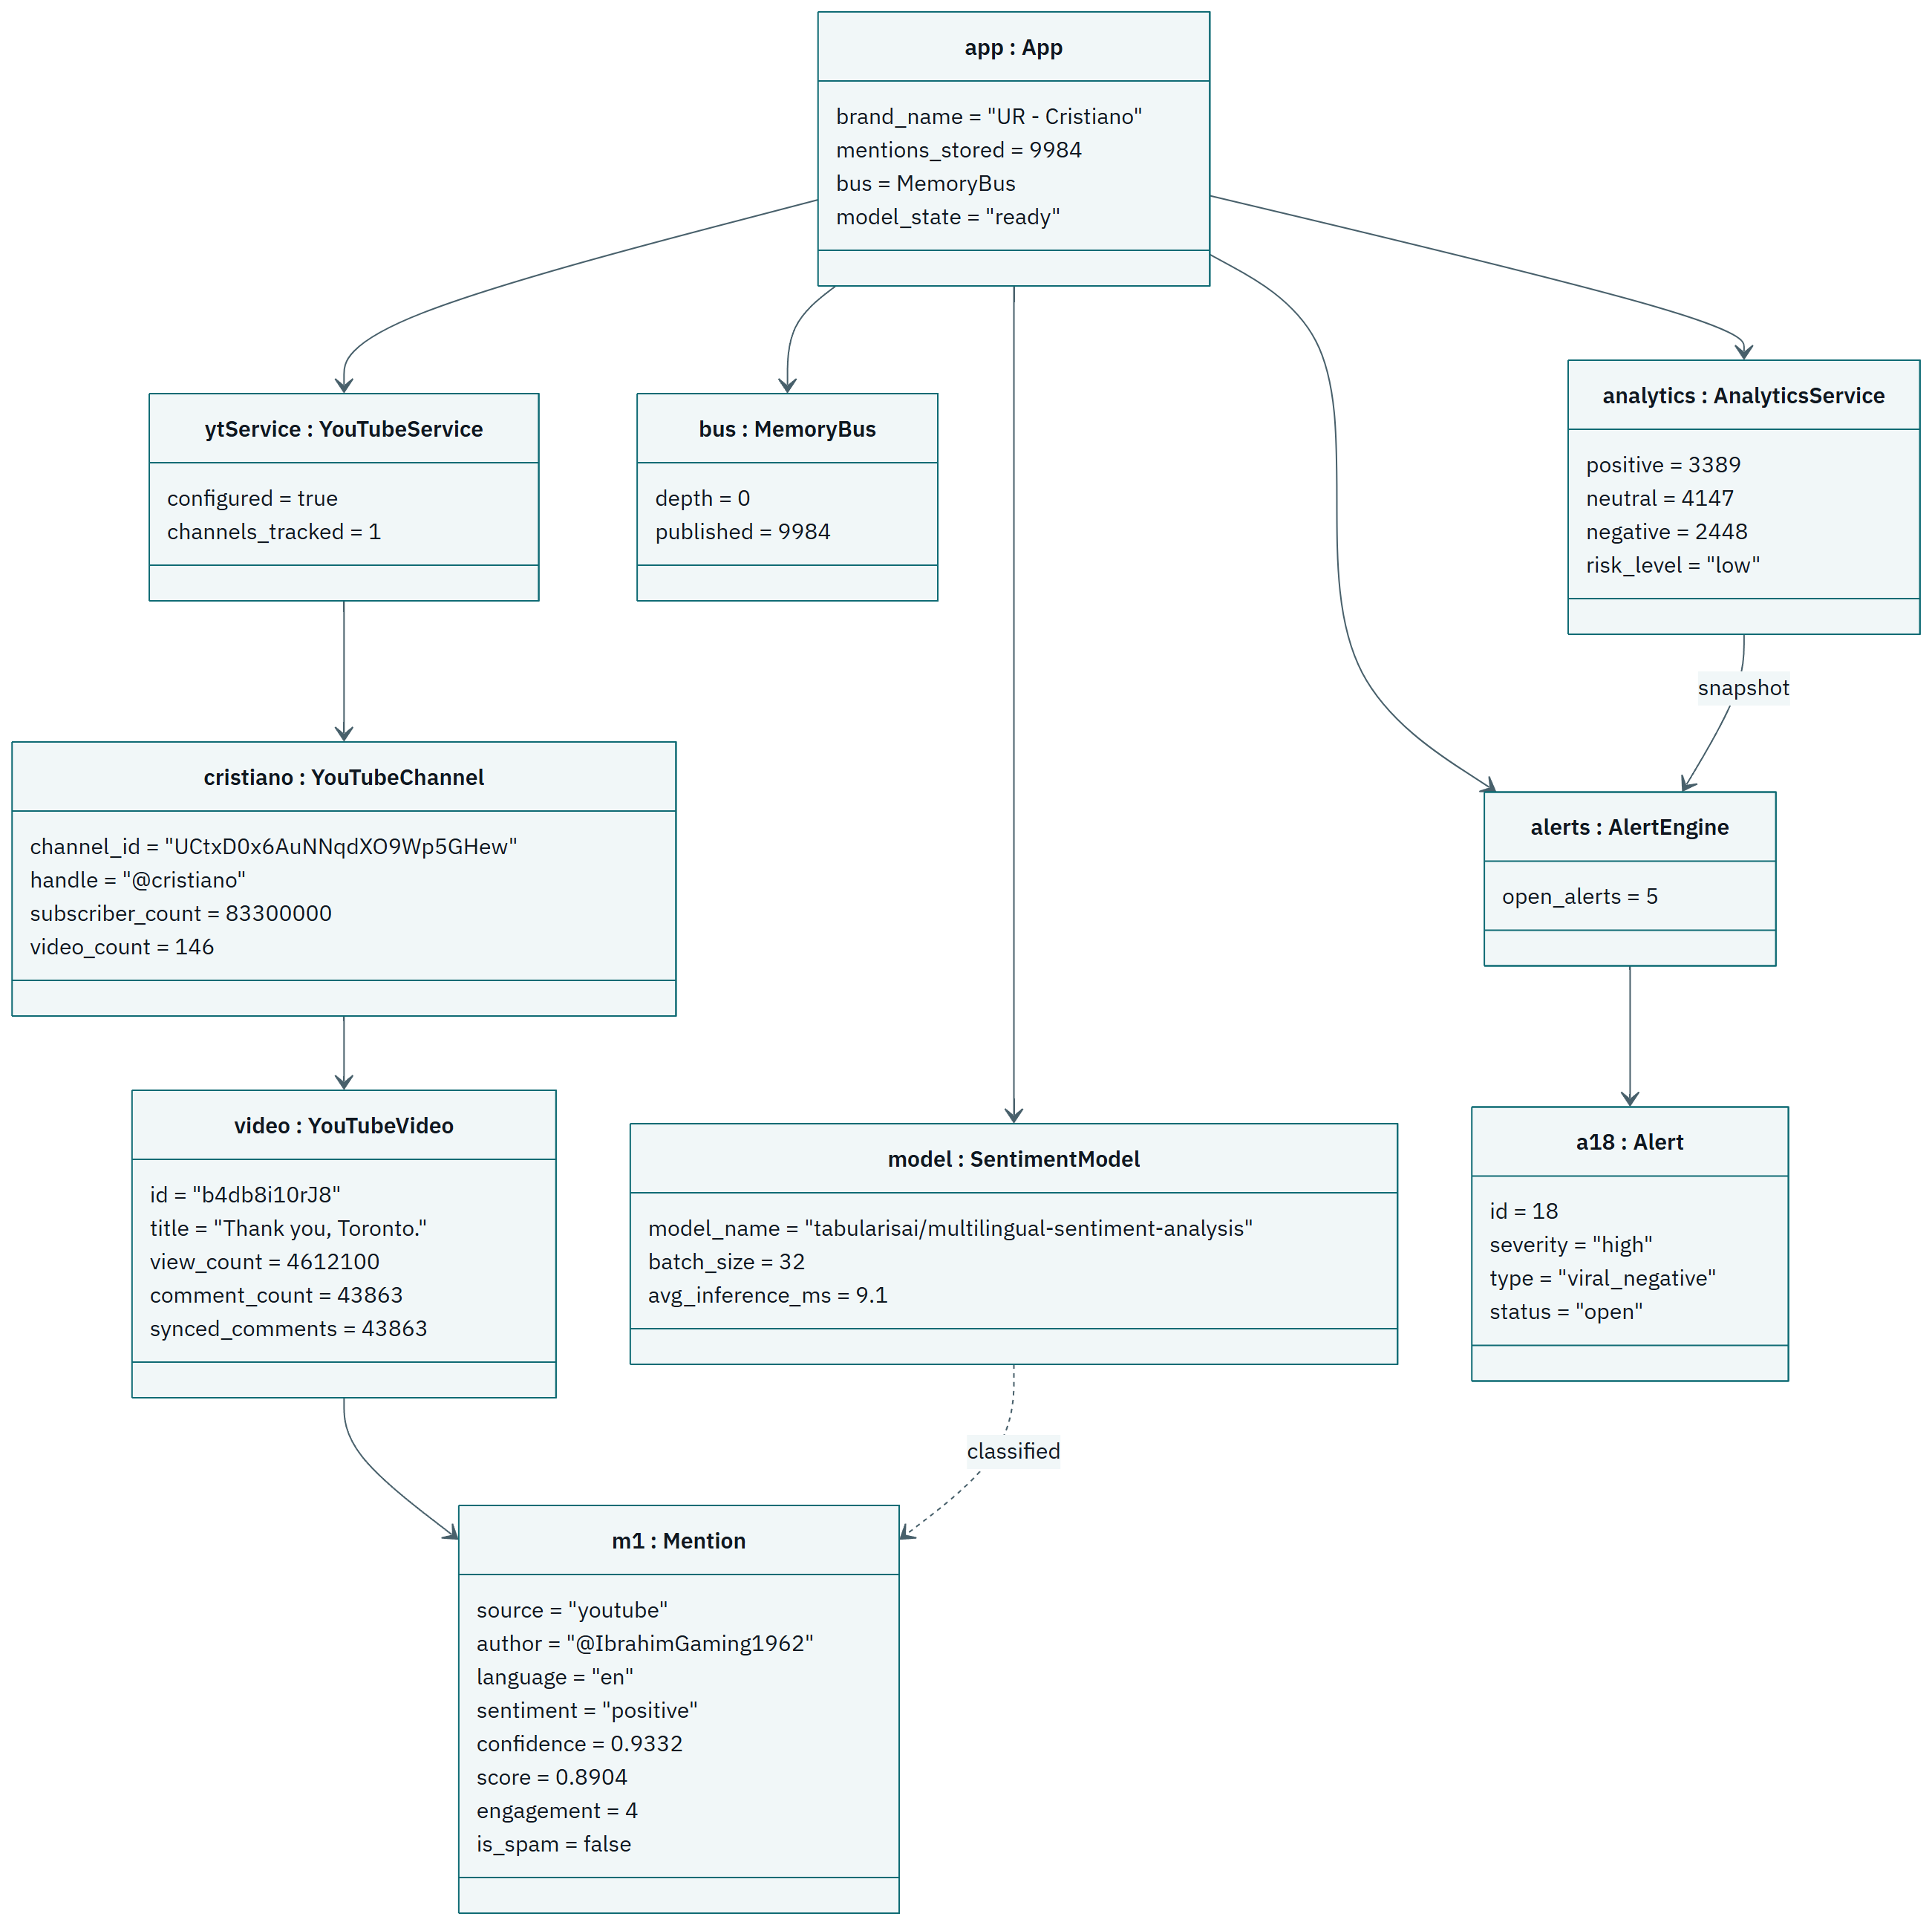
\includegraphics[width=0.95\linewidth, height=17cm, keepaspectratio]{figures/02-object-diagram.png}
\caption{Object Diagram (runtime snapshot)}
\label{fig:object}
\end{figure}

\textbf{Activity Diagram.} Figure~\ref{fig:activity} shows what happens to a single comment from the moment it is taken off the message bus until it appears on the dashboard.

\begin{figure}[!htbp]
\centering
\resizebox{!}{17.5cm}{%
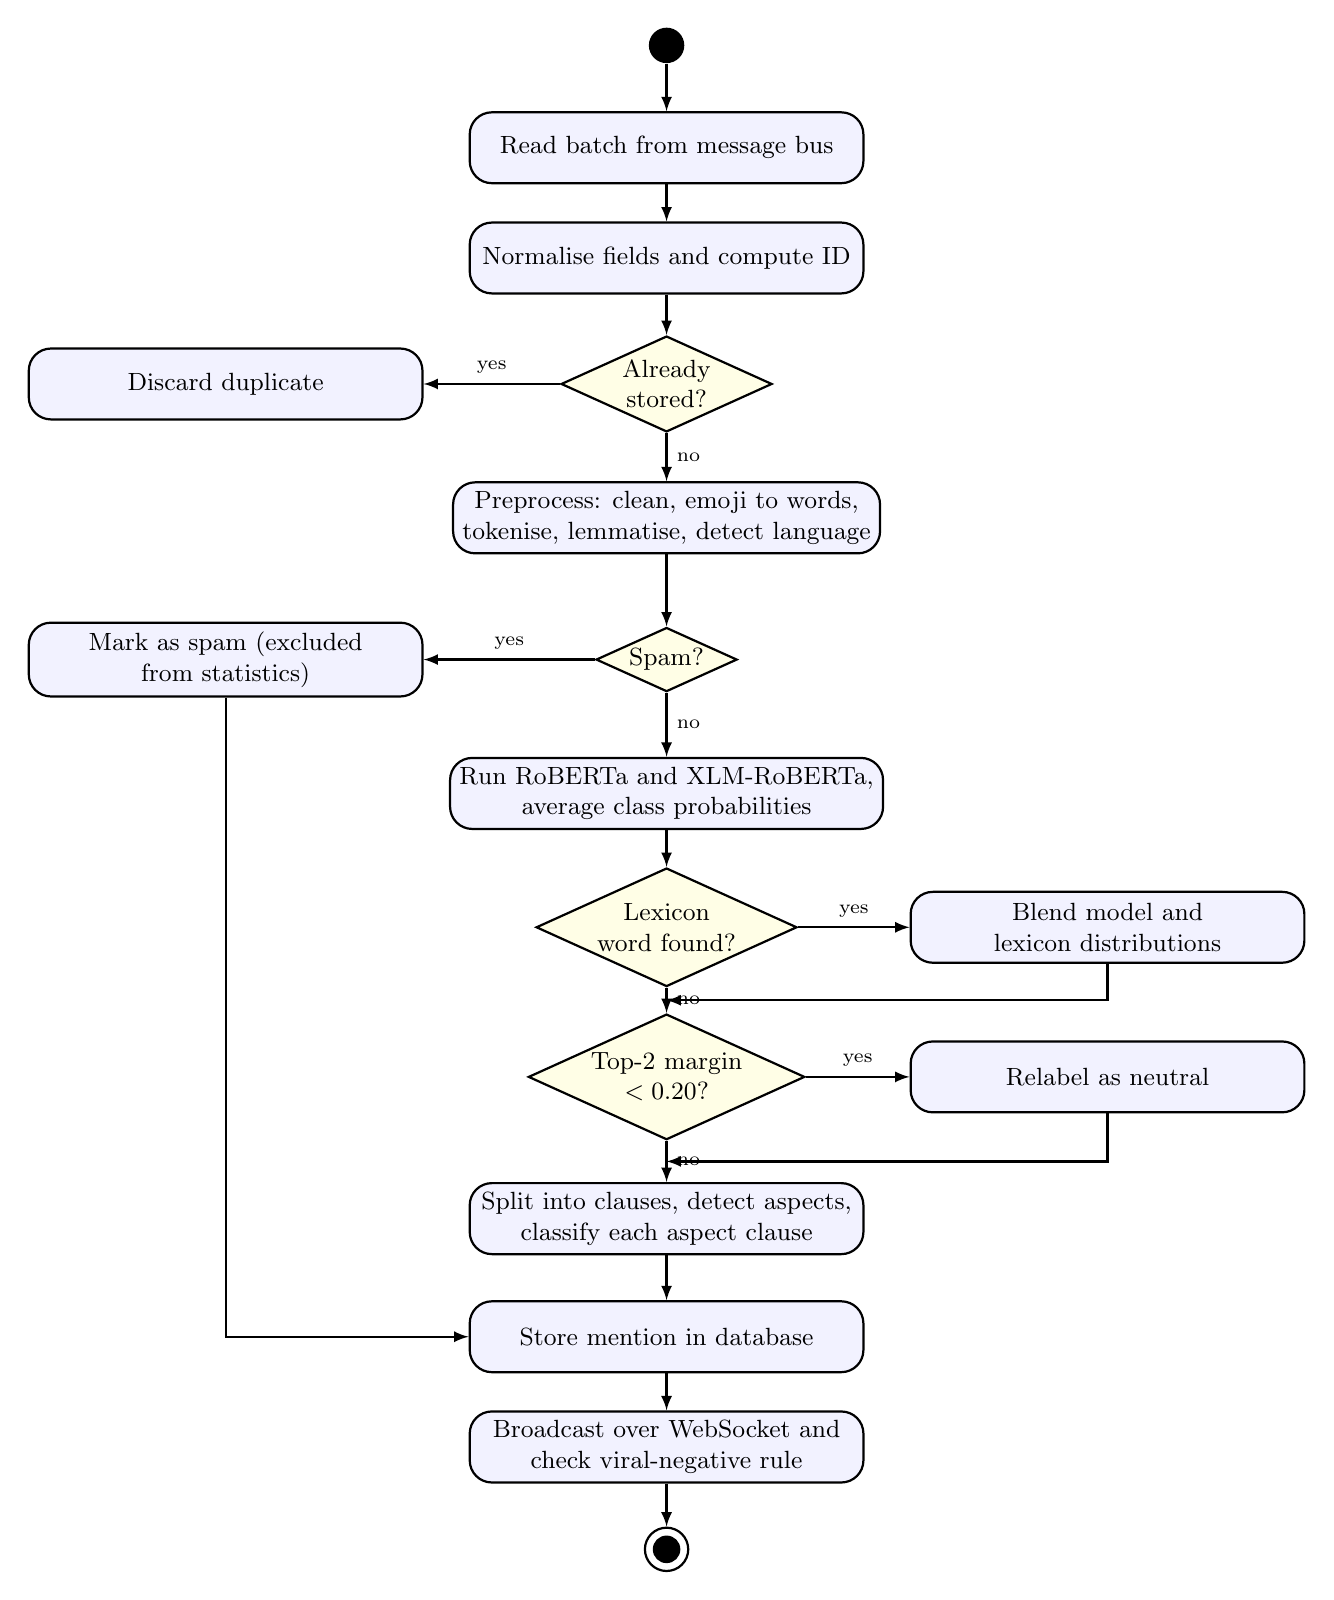
\begin{tikzpicture}[
    act/.style={draw, thick, rounded corners=8pt, minimum width=5cm, minimum height=0.9cm, align=center, font=\small, fill=blue!5},
    dec/.style={draw, thick, diamond, aspect=2.2, align=center, font=\small, fill=yellow!10, inner sep=1pt},
    arr/.style={->, >=latex, thick},
    lab/.style={font=\scriptsize}]
  \node[circle, fill=black, minimum size=0.45cm] (start) at (0,0) {};
  \node[act] (a1) at (0,-1.3) {Read batch from message bus};
  \node[act] (a2) at (0,-2.7) {Normalise fields and compute ID};
  \node[dec] (d1) at (0,-4.3) {Already\\stored?};
  \node[act] (a3) at (0,-6.0) {Preprocess: clean, emoji to words,\\tokenise, lemmatise, detect language};
  \node[dec] (d2) at (0,-7.8) {Spam?};
  \node[act] (a4) at (0,-9.5) {Run RoBERTa and XLM-RoBERTa,\\average class probabilities};
  \node[dec] (d3) at (0,-11.2) {Lexicon\\word found?};
  \node[act] (a5) at (5.6,-11.2) {Blend model and\\lexicon distributions};
  \node[dec] (d4) at (0,-13.1) {Top-2 margin\\$< 0.20$?};
  \node[act] (a6) at (5.6,-13.1) {Relabel as neutral};
  \node[act] (a7) at (0,-14.9) {Split into clauses, detect aspects,\\classify each aspect clause};
  \node[act] (a8) at (0,-16.4) {Store mention in database};
  \node[act] (a9) at (0,-17.8) {Broadcast over WebSocket and\\check viral-negative rule};
  \node[circle, draw, thick, minimum size=0.55cm] (end) at (0,-19.1) {};
  \node[circle, fill=black, minimum size=0.35cm] at (end) {};
  \node[act] (dup) at (-5.6,-4.3) {Discard duplicate};
  \node[act] (sp) at (-5.6,-7.8) {Mark as spam (excluded\\from statistics)};

  \draw[arr] (start) -- (a1);
  \draw[arr] (a1) -- (a2);
  \draw[arr] (a2) -- (d1);
  \draw[arr] (d1) -- node[lab, above]{yes} (dup);
  \draw[arr] (d1) -- node[lab, right]{no} (a3);
  \draw[arr] (a3) -- (d2);
  \draw[arr] (d2) -- node[lab, above]{yes} (sp);
  \draw[arr] (d2) -- node[lab, right]{no} (a4);
  \draw[arr] (sp.south) |- (a8.west);
  \draw[arr] (a4) -- (d3);
  \draw[arr] (d3) -- node[lab, above]{yes} (a5);
  \draw[arr] (a5.south) |- ($(d3.south)!0.5!(d4.north)$);
  \draw[arr] (d3) -- node[lab, right]{no} (d4);
  \draw[arr] (d4) -- node[lab, above]{yes} (a6);
  \draw[arr] (a6.south) |- ($(d4.south)!0.5!(a7.north)$);
  \draw[arr] (d4) -- node[lab, right]{no} (a7);
  \draw[arr] (a7) -- (a8);
  \draw[arr] (a8) -- (a9);
  \draw[arr] (a9) -- (end);
\end{tikzpicture}}
\caption{Activity Diagram - Processing of a Single Comment}
\label{fig:activity}
\end{figure}

\section{Tools and Technology Used}

\begin{table}[H]
\centering
\cellpadding
\caption{Tools and Technologies}
\label{tab:tools}
\begin{tabular}{|P{3.4cm}|P{3.8cm}|P{6.6cm}|}
\hline
\textbf{Area} & \textbf{Tool} & \textbf{Why we chose it} \\
\hline
Language & Python & The standard language for NLP and ML, with mature libraries \\
\hline
Web framework & FastAPI & Asynchronous, fast, built-in WebSocket support and automatic API documentation \\
\hline
Sentiment model & RoBERTa + XLM-RoBERTa ensemble (Cardiff NLP, Hugging Face); DistilBERT as fallback & BERT-family encoders fine-tuned on social-media text; multilingual; run on CPU \\
\hline
Deep learning runtime & PyTorch (CPU) & Required by the Transformers library; runs without a GPU \\
\hline
Text processing & NLTK, langdetect & Stop words, WordNet lemmatiser and language identification \\
\hline
Anomaly detection & scikit-learn & Reliable, well-documented Isolation Forest implementation \\
\hline
Forecasting & Prophet & Handles daily patterns and missing data, easy to interpret \\
\hline
Data handling & pandas, NumPy & Time bucketing and feature computation \\
\hline
Message bus & Apache Kafka / asyncio queue & Decouples collection from processing \\
\hline
Database & SQLite & Zero setup, single file, good enough for one brand \\
\hline
Frontend & React, Vite, Tailwind CSS & Fast development and a responsive, modern interface \\
\hline
Charts & Chart.js & Lightweight, interactive charts \\
\hline
Notifications & SMTP, Slack and Teams webhooks, Twilio & Reach the brand team wherever they already work \\
\hline
Version control & Git & Team collaboration and history \\
\hline
Deployment & Docker, systemd & Repeatable installation on a server \\
\hline
\end{tabular}
\end{table}

\section{Algorithm}
\label{sec:algo}

This section describes the three core algorithms of the system: the hybrid sentiment classifier, clause-level aspect extraction, and crisis detection using Isolation Forest.

\subsection{Hybrid Sentiment Classification}

\textbf{Operational mechanism.} Two BERT-family models score every comment: XLM-RoBERTa, which covers many languages, and RoBERTa, which is stronger on English social-media text. Each outputs probabilities for negative, neutral and positive, and we average the two distributions, giving $p_m = (p^+, p^0, p^-)$. If neither model can be loaded, the system falls back to multilingual DistilBERT, whose five ordinal classes are merged into three by adding neighbouring probabilities.

For code-mixed text we look up each token in a lexicon of Hinglish, Hindi and Marathi opinion words such as ``bekar'', ``bakwas'', ``mast'' and ``badhiya''. A negation word (``nahi'', ``not'', ``mat'') within two tokens flips the sign. The lexicon polarity $\ell \in [-1, 1]$ is the mean signed weight of the matched words. If at least one word matched, the two distributions are blended:
\be
p = (1-\lambda)\,p_m + \lambda\,p_\ell, \qquad \lambda = 0.35,
\ee
where $p_\ell = \big(\max(\ell,0),\; 1-|\ell|,\; \max(-\ell,0)\big)$.

While testing, we noticed that the model gives weak positive or negative labels to plain factual comments like ``ordered at 8 pm, arrived at 9''. So if the top class is not neutral, no lexicon word matched, and the two highest probabilities are close,
\be
p_{(1)} - p_{(2)} < \delta, \qquad \delta = 0.20,
\ee
the comment is relabelled as neutral. Finally, a continuous score $s = p^+ - p^-$ is stored with each comment and used in all analytics.

\begin{algorithm}[H]
\caption{Hybrid Sentiment Classification}
\KwIn{Comment text $x$, lexicon $L$, blend weight $\lambda$, margin $\delta$}
\KwOut{Label $y$, score $s$, probabilities $p$}
$x' \leftarrow$ Preprocess($x$)\;
\If{$x'$ is in cache}{\Return cached result\;}
$q_a \leftarrow$ XLM-RoBERTa($x'$); $q_b \leftarrow$ RoBERTa($x'$) \tcp*{3 class probabilities each}
$p_m \leftarrow \tfrac{1}{2}(q_a + q_b)$\;
$M \leftarrow$ tokens of $x'$ found in $L$, with negation applied\;
\eIf{$M \neq \emptyset$}{
  $\ell \leftarrow$ mean signed weight of $M$\;
  $p \leftarrow (1-\lambda)\,p_m + \lambda\,p_\ell$\;
}{
  $p \leftarrow p_m$\;
}
$y \leftarrow \arg\max p$\;
\If{$y \neq$ neutral \textbf{and} $M = \emptyset$ \textbf{and} $p_{(1)} - p_{(2)} < \delta$}{
  $y \leftarrow$ neutral\;
}
$s \leftarrow p^+ - p^-$\;
store $(y, s, p)$ in cache\;
\Return $(y, s, p)$\;
\end{algorithm}

\subsection{Clause-Level Aspect Extraction}

Each comment is split into clauses at sentence boundaries and at contrast words: ``but'', ``however'', ``although'', ``lekin'', ``magar'' and ``par''. Each clause is matched against the aspect lexicon using whole-word matching, which avoids silly mistakes such as finding ``late'' inside ``chocolate''. Every clause that mentions an aspect is then classified separately using the same sentiment model. The result is a list of (aspect, sentiment, score, evidence clause) entries for each comment.

\begin{algorithm}[H]
\caption{Clause-Level Aspect-Based Sentiment}
\KwIn{Comment text $x$, aspect lexicon $A = \{a_k : W_k\}$}
\KwOut{List $R$ of (aspect, label, score, clause)}
$C \leftarrow$ split $x$ at sentence ends and contrast words\;
$R \leftarrow \emptyset$\;
\ForEach{clause $c \in C$}{
  \ForEach{aspect $a_k$ with keyword set $W_k$}{
    \If{any $w \in W_k$ occurs in $c$ as a whole word}{
      $(y, s) \leftarrow$ HybridSentiment($c$)\;
      add $(a_k, y, s, c)$ to $R$\;
    }
  }
}
merge repeated aspects in $R$ by averaging their scores\;
\Return $R$\;
\end{algorithm}

\subsection{Isolation Forest Algorithm for Anomaly Detection}

\textbf{Operational mechanism.} Isolation Forest \cite{liu2008} is based on a simple idea: anomalies are few and different, so they are easier to separate from the rest of the data. The algorithm builds many random binary trees. At each node it picks a random feature and a random split value. A normal point, surrounded by many similar points, needs many splits before it ends up alone in a leaf. An anomalous point gets isolated after only a few splits. The average path length across all trees is turned into an anomaly score; shorter paths mean higher scores.

In our system, each data point is one 15-minute time bucket $t$, described by the feature vector
\be
f_t = \big\langle\, n_t,\; n^-_t,\; r_t,\; \bar{s}_t,\; \Delta n^-_t \,\big\rangle,
\ee
where $n_t$ is the number of mentions, $n^-_t$ the number of negative mentions, $r_t = n^-_t / n_t$ the negative share, $\bar{s}_t$ the mean sentiment score, and $\Delta n^-_t$ the change in negative count from the previous bucket.

\textbf{Why Isolation Forest alone is not enough.} Isolation Forest flags anything unusual, including a sudden burst of \textit{positive} comments after a good product launch. It also tends to flag the normal daily lunch and evening peaks, because during those hours the raw number of negative comments naturally goes up along with everything else. So we added a second, direction-aware check: a robust z-score of the negative share and negative count, computed against the median and median absolute deviation (MAD) of the previous $w$ buckets \cite{rousseeuw1993}:
\be
z_t = \frac{x_t - \mathrm{med}(x_{t-w:t-1})}{1.4826 \cdot \mathrm{MAD}(x_{t-w:t-1})}.
\ee
The median and MAD are used because, unlike the mean and standard deviation, they are not pulled upward by the very spikes we are trying to catch.

\textbf{Algorithmic workflow.} A bucket is declared a crisis only if (1) it has at least $n_{min} = 5$ negative mentions, and (2) either Isolation Forest flags it \textit{and} the negative share has risen by at least $\tau = 2.5$ robust standard deviations with the count also clearly up, or the negative share has risen very sharply ($1.6\tau$) with the count confirming it. Consecutive crisis buckets are merged into a single incident.

\textbf{Pseudocode.}

\begin{algorithm}[H]
\caption{Crisis Detection using Isolation Forest and Robust Z-Score}
\KwIn{Mentions from the last 72 h, bucket size $b = 15$ min, window $w$, threshold $\tau = 2.5$, minimum negatives $n_{min} = 5$, contamination $c = 0.05$}
\KwOut{Set of crisis buckets and incidents}
Group non-spam mentions into buckets of $b$ minutes\;
\ForEach{bucket $t$}{
  compute $n_t,\ n^-_t,\ r_t,\ \bar{s}_t,\ \Delta n^-_t$\;
}
\If{number of active buckets $\geq 24$}{
  Fit IsolationForest($c$) on feature vectors $f_t$\;
  $IF_t \leftarrow$ true if bucket $t$ is predicted as an outlier\;
}
\ForEach{bucket $t$}{
  $z^r_t \leftarrow$ robust z-score of $r_t$ over previous $w$ buckets\;
  $z^n_t \leftarrow$ robust z-score of $n^-_t$ over previous $w$ buckets\;
  $crisis_t \leftarrow (n^-_t \geq n_{min}) \wedge \big[(IF_t \wedge z^r_t \geq \tau \wedge z^n_t \geq 0.6\tau) \vee (z^r_t \geq 1.6\tau \wedge z^n_t \geq \tau)\big]$\;
}
Merge consecutive crisis buckets into incidents\;
\Return crisis buckets and incidents\;
\end{algorithm}

\subsection{Brand-Risk Score}

The risk score $R$ combines five signals, each scaled to the range 0 to 1:
\be
R = 35 f_1 + 20 f_2 + 25 f_3 + 10 f_4 + 10 f_5,
\ee
where $f_1$ is the recent negative share and its rise over the baseline, $f_2$ is how fast negative mentions are increasing, $f_3$ is the anomaly score when a crisis is detected, $f_4$ is the forecasted drop in sentiment over the next six hours, and $f_5$ is how concentrated the complaints are on a single aspect. The score is mapped to four levels: low (below 30), medium (30 to 54), high (55 to 74) and critical (75 and above). Because the weights add up to 100 and no single signal can push the score past 35, a high score only appears when several signals agree. In our experience this was the main reason the system did not raise false alarms.

%=====================================================================
\chapter{RESULTS AND DISCUSSION}

\section{Experimental Setup}

All experiments were run on the development laptop described in Table~\ref{tab:hw}, with the GPU deliberately disabled so that the numbers reflect CPU-only deployment. The backend ran as a single Uvicorn process with the in-memory message bus.

\subsection{Dataset}

We used four datasets, summarised in Table~\ref{tab:datasets}.

\begin{table}[H]
\centering
\cellpadding
\caption{Datasets Used for Evaluation}
\label{tab:datasets}
\begin{tabular}{|P{3.6cm}|P{1.8cm}|P{8.4cm}|}
\hline
\textbf{Dataset} & \textbf{Size} & \textbf{Description} \\
\hline
D1: Annotated benchmark & 83 & Brand comments labelled by our team as positive, neutral or negative. Deliberately includes English, Hinglish, Hindi in both scripts, Marathi, sarcasm, mixed opinions and spam. Aspect labels for 47 comments. \\
\hline
D2: Live corpus & 12,174 & Collected by the running system: 11,063 YouTube comments, 135 Instagram comments, 491 Google News articles, 483 App Store reviews and 2 rows imported from CSV. \\
\hline
D3: External validation & 483 & App Store reviews with reviewer-given star ratings: 1--2 stars treated as negative, 3 as neutral and 4--5 as positive. \\
\hline
D4: Real-comment benchmark & 200 & Comments sampled at random from the live database (110 YouTube, 60 Instagram, 30 news) and labelled by hand: 47 negative, 91 neutral, 62 positive. Unlike D1, these were not written or selected by the team. \\
\hline
\end{tabular}
\end{table}

An interesting finding from D2 was how multilingual even an ``English'' channel turned out to be. Language detection reported 8,144 English comments, but also 301 Indonesian, 207 Spanish, 139 Portuguese, 106 Italian and 100 Arabic comments, among others. This convinced us that a multilingual model is needed in practice and not just in theory.

\lofsection{Datasets}
\begin{figure}[!htbp]
\centering
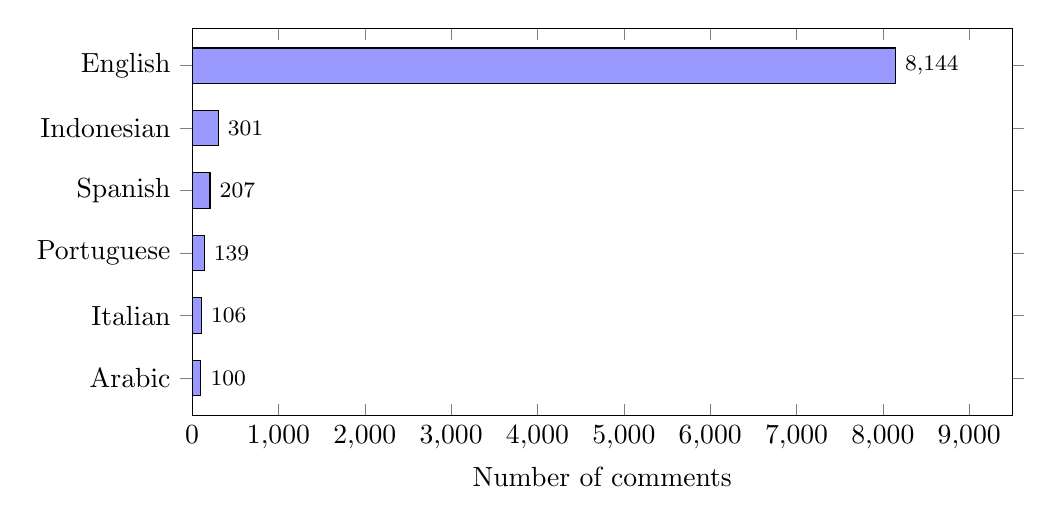
\begin{tikzpicture}
\begin{axis}[
    xbar, width=12cm, height=6.5cm,
    xlabel={Number of comments},
    symbolic y coords={Arabic, Italian, Portuguese, Spanish, Indonesian, English},
    ytick=data,
    nodes near coords, nodes near coords align={horizontal},
    xmin=0, xmax=9500,
    bar width=0.45cm,
    enlarge y limits=0.12,
    every node near coord/.append style={font=\footnotesize}]
\addplot[fill=blue!40] coordinates {(100,Arabic) (106,Italian) (139,Portuguese) (207,Spanish) (301,Indonesian) (8144,English)};
\end{axis}
\end{tikzpicture}
\caption{Language Distribution in the Live Corpus (top six languages)}
\label{fig:lang}
\end{figure}

\subsection{Performance Parameters}

We measured classification quality using accuracy, precision, recall and F1-score. For a class $c$, with $TP$, $FP$ and $FN$ the true positives, false positives and false negatives:
\begin{align}
\text{Precision}_c &= \frac{TP_c}{TP_c + FP_c}, \qquad \text{Recall}_c = \frac{TP_c}{TP_c + FN_c},\\
F1_c &= \frac{2 \cdot \text{Precision}_c \cdot \text{Recall}_c}{\text{Precision}_c + \text{Recall}_c}
\end{align}
Macro-averaged scores give each class equal weight, which matters here because our neutral class is smaller than the other two.

\textbf{Sentiment classification.} Table~\ref{tab:sentiment} compares the models we deployed on D1 (our benchmark) and D4 (real comments), and Figure~\ref{fig:modelcmp} adds the first model we tried.

\begin{table}[H]
\centering
\cellpadding
\caption{Sentiment Classification Results on D1 and D4}
\label{tab:sentiment}
\begin{tabular}{|P{1cm}|P{4.6cm}|c|c|c|c|}
\hline
\textbf{Set} & \textbf{Configuration} & \textbf{Accuracy} & \textbf{Macro-P} & \textbf{Macro-R} & \textbf{Macro-F1} \\
\hline
D1 & DistilBERT only & 0.7831 & 0.7735 & 0.7595 & 0.7647 \\
\hline
D1 & DistilBERT + lexicon (hybrid) & 0.7831 & 0.7838 & 0.7738 & 0.7764 \\
\hline
D1 & RoBERTa ensemble only & 0.8072 & 0.7918 & 0.7952 & 0.7904 \\
\hline
D1 & \textbf{RoBERTa ensemble + lexicon (deployed)} & \textbf{0.8313} & \textbf{0.8174} & \textbf{0.8238} & \textbf{0.8174} \\
\hline
D4 & DistilBERT + lexicon (hybrid) & 0.6650 & -- & -- & 0.6520 \\
\hline
D4 & \textbf{RoBERTa ensemble + lexicon (deployed)} & \textbf{0.7400} & \textbf{0.7844} & \textbf{0.7050} & \textbf{0.7276} \\
\hline
\end{tabular}
\end{table}

\begin{figure}[!htbp]
\centering
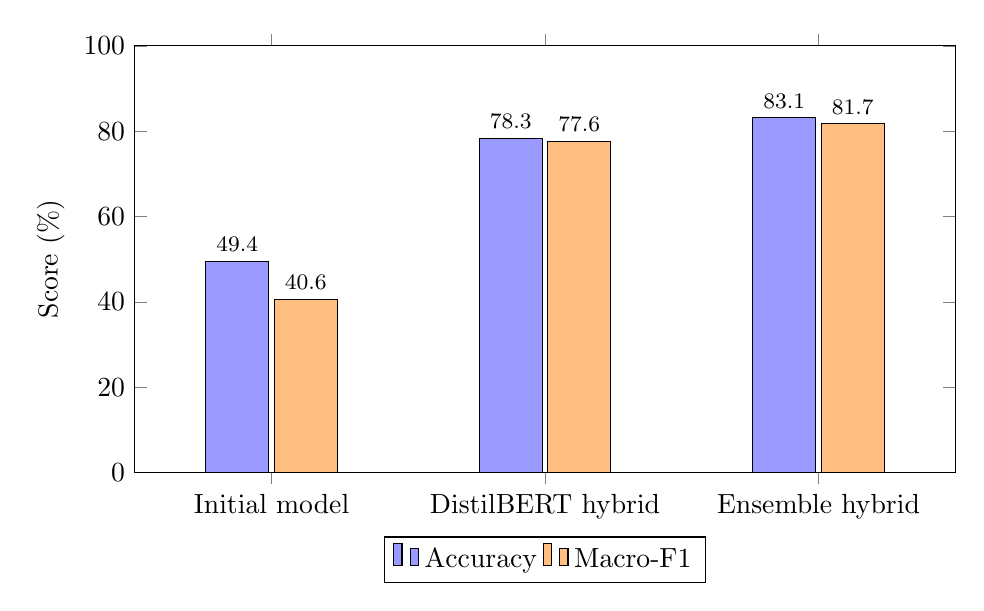
\begin{tikzpicture}
\begin{axis}[
    ybar, width=12cm, height=7cm,
    ylabel={Score (\%)},
    symbolic x coords={Initial model, DistilBERT hybrid, Ensemble hybrid},
    xtick=data, ymin=0, ymax=100,
    bar width=0.8cm,
    nodes near coords, every node near coord/.append style={font=\footnotesize},
    legend style={at={(0.5,-0.15)}, anchor=north, legend columns=2},
    enlarge x limits=0.25]
\addplot[fill=blue!40] coordinates {(Initial model,49.4) (DistilBERT hybrid,78.3) (Ensemble hybrid,83.1)};
\addplot[fill=orange!50] coordinates {(Initial model,40.6) (DistilBERT hybrid,77.6) (Ensemble hybrid,81.7)};
\legend{Accuracy, Macro-F1}
\end{axis}
\end{tikzpicture}
\caption{Comparison of Sentiment Models on D1}
\label{fig:modelcmp}
\end{figure}

On D1 the lexicon layer adds 2.4 points of accuracy and 2.7 points of macro-F1 to the ensemble; it changes few predictions, but they are the harder code-mixed ones. The transformer does most of the work. The more important result is on D4: DistilBERT, which looked good on our own benchmark, reached only 66.5\% on real comments, while the RoBERTa ensemble reached 74.0\%. Testing on real, unselected data is what exposed the weakness of the first deployed model.

\textbf{Per-class results.} Table~\ref{tab:perclass} and the confusion matrix in Table~\ref{tab:confusion} show how the hybrid classifier performs on each class.

\begin{table}[H]
\centering
\cellpadding
\caption{Per-Class Performance of the Deployed Classifier on D1}
\label{tab:perclass}
\begin{tabular}{|l|c|c|c|c|}
\hline
\textbf{Class} & \textbf{Precision} & \textbf{Recall} & \textbf{F1-score} & \textbf{Support} \\
\hline
Negative & 0.967 & 0.829 & 0.892 & 35 \\
\hline
Neutral & 0.652 & 0.750 & 0.698 & 20 \\
\hline
Positive & 0.833 & 0.893 & 0.862 & 28 \\
\hline
\end{tabular}
\end{table}

\begin{table}[H]
\centering
\cellpadding
\caption{Confusion Matrix of the Deployed Classifier on D1 (rows: true, columns: predicted)}
\label{tab:confusion}
\begin{tabular}{|l|c|c|c|}
\hline
 & \textbf{Negative} & \textbf{Neutral} & \textbf{Positive} \\
\hline
\textbf{Negative} & 29 & 5 & 1 \\
\hline
\textbf{Neutral} & 1 & 15 & 4 \\
\hline
\textbf{Positive} & 0 & 3 & 25 \\
\hline
\end{tabular}
\end{table}

For a reputation tool the most damaging mistake is calling a negative comment positive, because it hides an unhappy customer. This happened once in 35 negative comments on D1 and twice in 47 on D4; negative precision is 0.97 on D1 and 0.87 on D4, so when the system reports a complaint it is almost always one. The more common error is the opposite: mild complaints labelled neutral (19 of 47 negatives on D4). Neutral is the weakest class on D1, which is expected; the line between a factual statement and a mild opinion is blurry even for human annotators.

\textbf{Aspect detection.} On the 47 aspect-labelled comments in D1, aspect detection reached a precision of 0.900, recall of 0.730 and F1-score of 0.806. High precision means that when the system says a complaint is about delivery, it almost always is. Lower recall means some aspects are missed, mostly because the customer used a word that is not yet in the lexicon. Since users can extend the lexicon from the Settings page, recall can improve over time for a particular brand.

\textbf{External validation.} On D3, our predictions matched the star-based labels for 385 out of 483 reviews, an agreement of 79.7\%; the DistilBERT model we first deployed agreed on 74.7\% of the same reviews. These labels were given by the reviewers themselves, not by us, so this result gives some reassurance that the accuracy on D1 is not just a product of how we labelled our own data.

\textbf{Crisis detection.} In a controlled test, we injected a burst of delivery complaints into the live stream using the crisis simulator, on top of the real data. The first alert, ``sudden spike in negative sentiment'', was raised 24 seconds after the burst began, at critical severity, and the risk score rose from 20 to 79 out of 100. In the same evaluation cycle the system also raised a risk-threshold alert, a negative-share alert and an aspect-surge alert for delivery, and Isolation Forest gave the window an anomaly score of 1.00, with 84\% of its mentions negative. When the test was repeated while earlier alerts of the same types were less than 30 minutes old, those alerts were held back by the cool-down as intended, so one incident did not produce a stream of repeated alerts.

We also checked the effect of our main design decision in the detector. With a simple rule based on the raw negative count, the detector flagged four extra windows over a three-day period in which the negative share was close to normal (about 30\% against a 20\% baseline) and only the volume had risen with ordinary daily traffic. Switching to the negative share as the main signal removed all four false alarms and still caught the real incident.

\lofsection{Results}
\begin{figure}[!htbp]
\centering
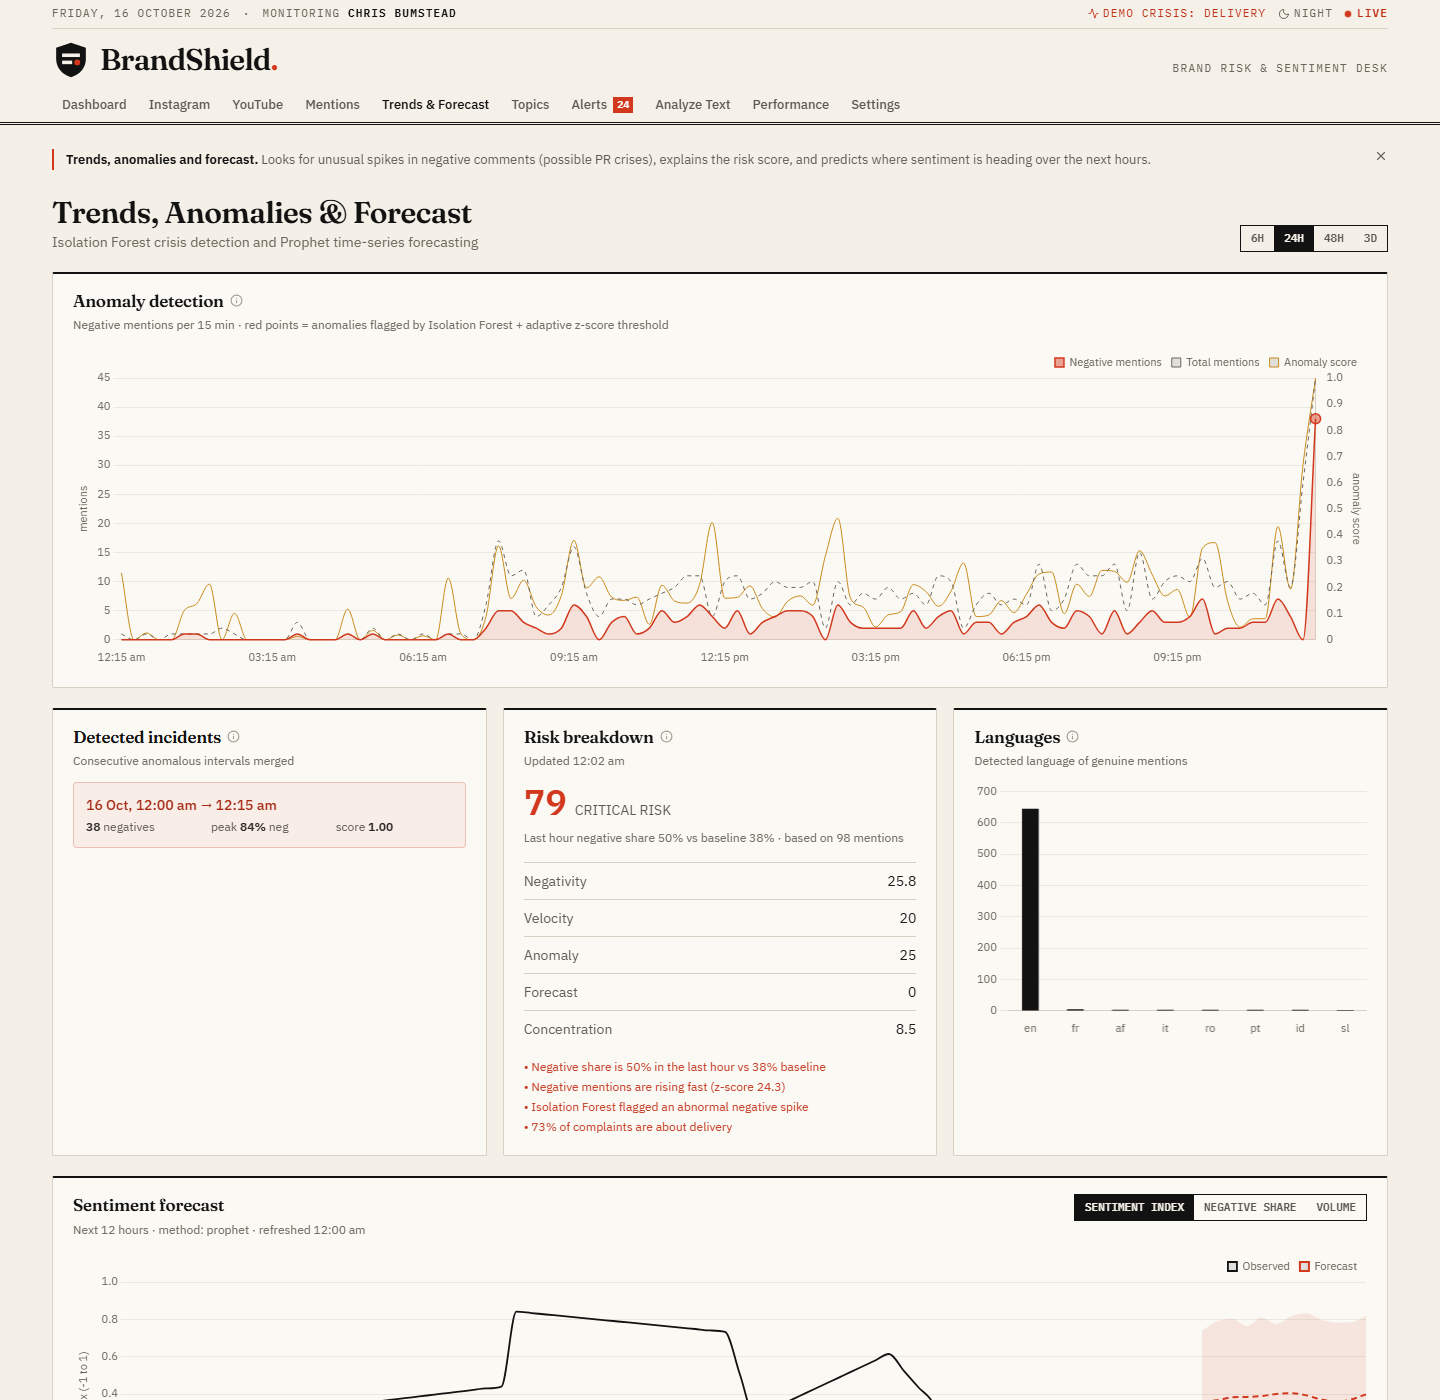
\includegraphics[width=\linewidth,height=0.45\textheight,keepaspectratio]{figures/ui-crisis.png}
\caption{Crisis Simulation - Detected Incident on the Trends Page}
\label{fig:crisis}
\end{figure}

\subsection{Efficiency Issues}

\begin{table}[H]
\centering
\cellpadding
\caption{Efficiency Measurements}
\label{tab:efficiency}
\begin{tabular}{|P{6cm}|P{3.4cm}|P{4.4cm}|}
\hline
\textbf{Metric} & \textbf{Value} & \textbf{Conditions} \\
\hline
Inference time per comment & 32.4 ms (D1), 120 ms (D4) & Batch of 32, two models, laptop CPU; D4 comments are longer \\
\hline
Single comment (Analyze Text) & about 140 ms & Including HTTP overhead \\
\hline
Memory used by running system & about 2 GB & Model loaded, live data \\
\hline
Crisis detection delay & about 25 s & Controlled injection \\
\hline
YouTube API calls on unchanged videos & 0 & Repeated sync \\
\hline
\end{tabular}
\end{table}

During development we ran into a few efficiency problems worth mentioning:

\begin{itemize}
    \item \textbf{Blocking the server.} Our first version ran model inference directly inside the asynchronous event loop. While a large batch was being processed, the dashboard froze. Moving all CPU-heavy work (inference, pandas, Isolation Forest, Prophet) to worker threads fixed this.
    \item \textbf{YouTube quota.} The free YouTube Data API key allows 10,000 units a day. Our first synchronisation logic re-downloaded every comment on every poll and would have used up the quota within hours. The fix was to compare each video's comment count with the number already synced, and only fetch comments for videos that changed.
    \item \textbf{Repeated comments.} Social media is full of identical comments (``first'', ``nice video'', copied spam). A cache of 50,000 entries keyed on normalised text avoids running the model on the same text twice.
    \item \textbf{Model download size.} The two models together are about 1.6 GB and are downloaded on first start. Until it finishes, the API stays up but returns a clear ``model loading'' message instead of failing.
\end{itemize}

\section{Software Testing}

Testing so far has been a combination of scripted model evaluation, manual API testing through the built-in Swagger interface at \texttt{/docs}, and manual testing of the dashboard during development and demonstrations. Some components, such as preprocessing, spam detection, timestamp parsing and settings validation, were also checked by running them directly on sample inputs. The API test cases are also automated in a script (\texttt{backend/scripts/smoke\_test.py}) that runs them against the live server and cleans up its own test data.

\subsection{Test Cases and Test Results}

Table~\ref{tab:testcases} lists the test cases. All test cases were executed on the final system, with the two-model ensemble loaded and live data.

\begin{longtable}{|P{1.2cm}|P{3.6cm}|P{3.4cm}|P{3.6cm}|P{1.6cm}|}
\caption{Test Case Summary}
\label{tab:testcases}\\
\hline
\textbf{TC ID} & \textbf{Description} & \textbf{Input} & \textbf{Expected Result} & \textbf{Status} \\
\hline
\endfirsthead
\hline
\textbf{TC ID} & \textbf{Description} & \textbf{Input} & \textbf{Expected Result} & \textbf{Status} \\
\hline
\endhead
TC-01 & Health check & GET \texttt{/api/health} & 200, status ``ok'' & Pass \\ \hline
TC-02 & Request before model is ready & POST \texttt{/api/analyze} right after start & 503 until model ready, then 200 & Pass \\ \hline
TC-03 & Text length validation & Empty text; 5001 characters & 422 for both & Pass \\ \hline
TC-04 & English negative comment & ``Worst coffee ever'' with angry emoji & Negative, score $< 0$ & Pass \\ \hline
TC-05 & Hinglish negative comment & ``khana ekdum bekar tha'' & Negative, lexicon polarity $< 0$ & Pass \\ \hline
TC-06 & Mixed opinion & ``the product is great but delivery was late'' & Product positive, delivery negative & Pass \\ \hline
TC-07 & Promotional spam & ``Follow me for free followers!!!'' with link & Spam, promotional phrase & Pass \\ \hline
TC-08 & Link-only spam & ``https://bit.ly/abc'' & Spam, link with little content & Pass \\ \hline
TC-09 & Preprocessing & ``Coffee was sooooo good @saffron \#yum'' with emoji & Repeated letters shortened, mention removed, hashtag unwrapped, emoji mapped to a word & Pass \\ \hline
TC-10 & Empty ingest & POST \texttt{/ingest} with empty list & 422 & Pass \\ \hline
TC-11 & Duplicate ingest & Same item sent twice & Stored once, duplicate counter +1 & Pass \\ \hline
TC-13 & Invalid CSV & UTF-16 file; file without text column & 400 with clear message & Pass \\ \hline
TC-14 & CSV engagement parsing & Values ``1e3'', ``-4'', ``35'' & 0, 0, 35 & Pass \\ \hline
TC-15 & Bad timestamps & ``garbage''; a date in 2030 & Both stored with ingestion time & Pass \\ \hline
TC-16 & Settings validation & Invalid threshold values & 422 with field message & Pass \\ \hline
TC-18 & Crisis detection & Delivery crisis, 20 min, intensity 0.8 & Spike and aspect-surge alerts; anomaly visible & Pass (24 s) \\ \hline
TC-19 & Alert de-duplication & Keep crisis running after first alert & No duplicate alert within 30 min & Pass \\ \hline
TC-20 & Forecast fallback & Empty DB; $<$ 36 h; $\geq$ 36 h history & insufficient data / Holt / Prophet & Pass \\ \hline
TC-22 & Alert actions & Acknowledge an alert; unknown ID & 200 with live update; 404 & Pass \\ \hline
TC-23 & Slack notification & Configure webhook, send test & Delivered; invalid URL reports error & Pass \\ \hline
TC-24 & Remote setup blocked & PUT \texttt{/keys} with forwarded header & 403 & Pass \\ \hline
TC-26 & Add YouTube channel & Valid handle; non-existent handle & Channel stored; 422 & Pass \\ \hline
TC-28 & WebSocket & Open \texttt{/ws}, send ``ping'' & Status message, then ``pong'' & Pass \\ \hline
TC-29 & Model evaluation & Run evaluation script & Metrics saved and reproducible & Pass \\ \hline
TC-30 & Kafka fallback & Kafka configured, no broker & Starts on memory bus & Pass \\ \hline
TC-31 & Token privacy & GET \texttt{/instagram/status} & No access token in response & Pass \\ \hline
\end{longtable}

\section{Summary}

\subsection{Result Analysis and Discussion}

Looking at the results as a whole, three things stand out to us.

First, \textbf{aspect-level output changes what a manager can do with the numbers}. A dashboard that says ``35\% negative'' starts a discussion; a dashboard that says ``35\% negative, and 70\% of those complaints are about delivery'' tells someone what to fix. The relatively high precision of aspect detection (0.90) means these attributions can be trusted when they appear.

Second, \textbf{knowing the direction of an anomaly matters more than how sophisticated the detector is}. Isolation Forest on its own was not what made crisis detection usable. Using the negative \textit{share} as the main signal, and only alerting when it rises, was the change that removed false alarms.

Third, \textbf{CPU-only operation is realistic}. The ensemble costs about three times as much compute as DistilBERT, but at 32--120 ms per comment it still analyses several hundred comments a minute on a laptop CPU, far more than a single brand receives, without a GPU.

At the same time, the results have clear limits. D1 has only 83 comments labelled by our own team and D4 has 200 labelled by one annotator, so the confidence intervals are wide (about $\pm$6 points on D4) and the small improvement from the lexicon layer is not statistically proven. Sarcasm (``Well done Apple, only three years late'') and mild complaints are still the most common errors. Comments that mix praise and complaint are usually labelled negative overall, even though the aspect-level output is correct. Some Hinglish complaints about price, such as ``bahut mehenga hai'', are still missed. And the 25-second detection time was measured on a sharp, injected surge; real crises build up more gradually, so it should be seen as a best case. These points are the starting list for our future work.

%=====================================================================
\chapter{CONCLUSION AND \vspace*{0.5\baselineskip} FUTURE WORK}

\section{Conclusions}

In this project we designed and built BrandShield AI, a real-time system that listens to what customers say about a brand on social media and turns it into something a brand team can act on. The system collects comments from YouTube, Instagram, Google News and the App Store, classifies them with an ensemble of BERT-family models (RoBERTa and XLM-RoBERTa) supported by a Hinglish, Hindi and Marathi lexicon, explains opinions at the level of business aspects, detects harmful surges in negativity using Isolation Forest and a robust share-based threshold, forecasts where sentiment is heading, and raises alerts through a live dashboard and external channels.

Our evaluation shows 83.1\% accuracy and 81.7\% macro-F1 on our multilingual benchmark, 74.0\% accuracy on 200 randomly sampled real comments (up from 66.5\% with the DistilBERT model we first deployed), an aspect detection F1 of 0.806, and 79.7\% agreement with independent star ratings. The system has analysed more than 12,000 real comments on an ordinary laptop CPU and detected a simulated complaint wave in under half a minute.

Beyond the numbers, the project taught us that the most valuable decisions were often simple ones: picking the right base model, measuring on our own data instead of trusting benchmark claims, and thinking carefully about what kind of change is actually a problem for a brand.

\section{Future Work}

\begin{itemize}
    \item \textbf{Larger evaluation set.} Build a labelled dataset of several hundred comments with multiple annotators and report inter-annotator agreement.
    \item \textbf{Better code-mixed handling.} Fine-tune the model on domain-specific Hinglish comments instead of only correcting it afterwards, with special attention to price complaints and mixed opinions.
    \item \textbf{Smarter aspect extraction.} Replace or complement the keyword lexicon with a few-shot or prompt-based extractor, so that new vocabulary is picked up without manual lexicon updates.
    \item \textbf{Real crisis evaluation.} Test detection delay on documented real-world brand incidents rather than injected ones.
    \item \textbf{Multi-user support.} Add login, roles and per-brand data isolation so that one installation can serve several teams.
    \item \textbf{Scalable storage.} Move from SQLite to PostgreSQL or TimescaleDB for larger deployments with concurrent writers.
    \item \textbf{Automated testing.} Add a pytest suite and continuous integration covering the test cases in Table~\ref{tab:testcases}.
    \item \textbf{Data retention policy.} Automatically archive or delete old mentions and alerts.
\end{itemize}

\section{Application}

\begin{itemize}
    \item \textbf{Small and medium businesses:} restaurants, cafes, local retail chains and D2C brands that cannot afford enterprise listening tools.
    \item \textbf{Food delivery and e-commerce:} catching delivery, packaging and refund complaints early, before they spread.
    \item \textbf{App developers:} monitoring app store reviews after a new release to spot bugs and crashes quickly.
    \item \textbf{YouTube creators and influencers:} understanding how their audience reacts to each video, and spotting backlash early.
    \item \textbf{Marketing and PR agencies:} tracking campaign reception for clients in near real time.
    \item \textbf{Public sector and services:} following public feedback on a service, scheme or announcement in regional languages.
\end{itemize}

\clearpage
\pagenumbering{gobble}
\pagestyle{empty}

\makeatletter
\renewcommand{\@chapapp}{Annexure}
\renewcommand{\thechapter}{\Alph{chapter}}
\makeatother

\makeatletter
\renewcommand{\@makechapterhead}[1]{%
  \vspace*{\fill}%
  \begin{center}
    {\Huge\bfseries Annexure \thechapter\\[1.5ex]#1}
  \end{center}
  \thispagestyle{chaptertitle}%
  \vspace*{\fill}
  \clearpage
}
\makeatother

\begin{appendices}
\chapter{References}
% Remove any automatic bibliography title and formatting
\makeatletter
\renewenvironment{thebibliography}[1]
     {\list{\@biblabel{\@arabic\c@enumiv}}%
           {\settowidth\labelwidth{\@biblabel{#1}}%
            \leftmargin\labelwidth
            \advance\leftmargin\labelsep
            \@openbib@code
            \usecounter{enumiv}%
            \let\p@enumiv\@empty
            \renewcommand\theenumiv{\@arabic\c@enumiv}}%
      \sloppy
      \clubpenalty4000
      \@clubpenalty \clubpenalty
      \widowpenalty4000%
      \sfcode`\.\@m}
     {\def\@noitemerr
       {\@latex@warning{Empty `thebibliography' environment}}%
      \endlist}
\makeatother
\begin{thebibliography}{99}
% Chicago style references

\bibitem{vaswani2017}
Vaswani, Ashish, Noam Shazeer, Niki Parmar, Jakob Uszkoreit, Llion Jones, Aidan N. Gomez, Lukasz Kaiser, and Illia Polosukhin. ``Attention Is All You Need.'' In \textit{Advances in Neural Information Processing Systems 30 (NeurIPS)}, 5998--6008. 2017.

\bibitem{devlin2019}
Devlin, Jacob, Ming-Wei Chang, Kenton Lee, and Kristina Toutanova. ``BERT: Pre-training of Deep Bidirectional Transformers for Language Understanding.'' In \textit{Proceedings of NAACL-HLT 2019}, 4171--4186. 2019.

\bibitem{sanh2019}
Sanh, Victor, Lysandre Debut, Julien Chaumond, and Thomas Wolf. ``DistilBERT, a Distilled Version of BERT: Smaller, Faster, Cheaper and Lighter.'' \textit{arXiv preprint arXiv:1910.01108} (2019).

\bibitem{liu2019roberta}
Liu, Yinhan, Myle Ott, Naman Goyal, Jingfei Du, Mandar Joshi, Danqi Chen, Omer Levy, Mike Lewis, Luke Zettlemoyer, and Veselin Stoyanov. ``RoBERTa: A Robustly Optimized BERT Pretraining Approach.'' \textit{arXiv preprint arXiv:1907.11692} (2019).

\bibitem{conneau2020}
Conneau, Alexis, Kartikay Khandelwal, Naman Goyal, Vishrav Chaudhary, Guillaume Wenzek, Francisco Guzm\'an, Edouard Grave, Myle Ott, Luke Zettlemoyer, and Veselin Stoyanov. ``Unsupervised Cross-lingual Representation Learning at Scale.'' In \textit{Proceedings of the 58th Annual Meeting of the ACL}, 8440--8451. 2020.

\bibitem{barbieri2022}
Barbieri, Francesco, Luis Espinosa Anke, and Jose Camacho-Collados. ``XLM-T: Multilingual Language Models in Twitter for Sentiment Analysis and Beyond.'' In \textit{Proceedings of the Thirteenth Language Resources and Evaluation Conference (LREC)}. 2022.

\bibitem{loureiro2022}
Loureiro, Daniel, Francesco Barbieri, Leonardo Neves, Luis Espinosa Anke, and Jose Camacho-Collados. ``TimeLMs: Diachronic Language Models from Twitter.'' In \textit{Proceedings of the 60th Annual Meeting of the ACL: System Demonstrations}. 2022.

\bibitem{barbieri2020}
Barbieri, Francesco, Jose Camacho-Collados, Luis Espinosa-Anke, and Leonardo Neves. ``TweetEval: Unified Benchmark and Comparative Evaluation for Tweet Classification.'' In \textit{Findings of the Association for Computational Linguistics: EMNLP 2020}, 1644--1650. 2020.

\bibitem{pang2002}
Pang, Bo, Lillian Lee, and Shivakumar Vaithyanathan. ``Thumbs up? Sentiment Classification using Machine Learning Techniques.'' In \textit{Proceedings of EMNLP 2002}, 79--86. 2002.

\bibitem{liu2012}
Liu, Bing. \textit{Sentiment Analysis and Opinion Mining}. Synthesis Lectures on Human Language Technologies. Morgan \& Claypool Publishers, 2012.

\bibitem{hutto2014}
Hutto, C. J., and Eric Gilbert. ``VADER: A Parsimonious Rule-Based Model for Sentiment Analysis of Social Media Text.'' In \textit{Proceedings of the Eighth International AAAI Conference on Weblogs and Social Media (ICWSM)}. 2014.

\bibitem{joshi2016}
Joshi, Aditya, Ameya Prabhu, Manish Shrivastava, and Vasudeva Varma. ``Towards Sub-Word Level Compositions for Sentiment Analysis of Hindi-English Code Mixed Text.'' In \textit{Proceedings of COLING 2016}, 2482--2491. 2016.

\bibitem{patwa2020}
Patwa, Parth, Gustavo Aguilar, Sudipta Kar, Suraj Pandey, Srinivas PYKL, Bj\"orn Gamb\"ack, Tanmoy Chakraborty, Thamar Solorio, and Amitava Das. ``SemEval-2020 Task 9: Overview of Sentiment Analysis of Code-Mixed Tweets.'' In \textit{Proceedings of the Fourteenth Workshop on Semantic Evaluation}, 774--790. 2020.

\bibitem{pontiki2014}
Pontiki, Maria, Dimitris Galanis, John Pavlopoulos, Harris Papageorgiou, Ion Androutsopoulos, and Suresh Manandhar. ``SemEval-2014 Task 4: Aspect Based Sentiment Analysis.'' In \textit{Proceedings of the 8th International Workshop on Semantic Evaluation (SemEval 2014)}, 27--35. 2014.

\bibitem{liu2008}
Liu, Fei Tony, Kai Ming Ting, and Zhi-Hua Zhou. ``Isolation Forest.'' In \textit{Proceedings of the Eighth IEEE International Conference on Data Mining (ICDM)}, 413--422. 2008.

\bibitem{chandola2009}
Chandola, Varun, Arindam Banerjee, and Vipin Kumar. ``Anomaly Detection: A Survey.'' \textit{ACM Computing Surveys} 41, no. 3 (2009): 1--58.

\bibitem{rousseeuw1993}
Rousseeuw, Peter J., and Christophe Croux. ``Alternatives to the Median Absolute Deviation.'' \textit{Journal of the American Statistical Association} 88, no. 424 (1993): 1273--1283.

\bibitem{taylor2018}
Taylor, Sean J., and Benjamin Letham. ``Forecasting at Scale.'' \textit{The American Statistician} 72, no. 1 (2018): 37--45.

\bibitem{hyndman2021}
Hyndman, Rob J., and George Athanasopoulos. \textit{Forecasting: Principles and Practice}. 3rd ed. Melbourne: OTexts, 2021.

\bibitem{kreps2011}
Kreps, Jay, Neha Narkhede, and Jun Rao. ``Kafka: A Distributed Messaging System for Log Processing.'' In \textit{Proceedings of the NetDB Workshop}. 2011.

\bibitem{wolf2020}
Wolf, Thomas, et al. ``Transformers: State-of-the-Art Natural Language Processing.'' In \textit{Proceedings of EMNLP 2020: System Demonstrations}, 38--45. 2020.

\end{thebibliography}


\chapter{Plagiarism Report}
\begin{center}
\screenshot{Plagiarism report (to be attached after checking the final report)}{18cm}
\end{center}

\chapter{Paper Published (if any)}
\noindent A research paper based on this work, titled \textit{``BrandShield AI: A Real-Time Multilingual Pipeline for Aspect-Based Brand Sentiment Analysis and Crisis Detection on Social Media''}, is currently being prepared. Publication details will be added here once it is submitted and accepted.

\chapter{Sponsorship detail (if any)}
\noindent Not applicable. This project is not sponsored.
\end{appendices}
\end{document}
